\documentclass[sigplan,9pt]{acmart}

\usepackage{paralist}

\usepackage{amssymb, amsmath}
\usepackage{enumitem}
\usepackage{todonotes}
\usepackage{subcaption}
\captionsetup{compatibility=false}
\usepackage{url}
\usepackage{graphicx}
\usepackage{xcolor}
\usepackage{centernot}
%\usepackage{rotating}
\usepackage{tikz}
\graphicspath{{figures/}}
\usetikzlibrary{calc,trees,positioning,arrows,chains,automata,shapes.geometric,%
    decorations.pathreplacing,decorations.pathmorphing,shapes,%
    matrix,shapes.symbols}

\usetikzlibrary{shapes,arrows,automata,positioning,calc}
\usetikzlibrary{fit,backgrounds}
\usetikzlibrary{decorations.pathreplacing}
\tikzset{
>=stealth',
  punktchain/.style={
    rectangle,
    rounded corners,
    % fill=black!10,
    draw=black, very thick,
    text width=6em,
    minimum height=3em,
    text centered,
    on chain},
  line/.style={draw, thick, <-},
  element/.style={
    tape,
    top color=white,
    bottom color=blue!50!black!60!,
    minimum width=8em,
    draw=blue!40!black!90, very thick,
    text width=10em,
    minimum height=3.5em,
    text centered,
    on chain},
  every join/.style={->, thick,shorten >=1pt},
  decoration={brace},
  tuborg/.style={decorate},
  tubnode/.style={midway, right=2pt},
}

%\newcommand*\InputTable[1]{\input{tables/#1.tex}}
%\newcommand*\InputTikz[1]{\input{figures/#1.tex}}
\newif\iflong
%\longtrue
\longfalse

\newif\ifshort
\shorttrue
%\shortfalse

\usepackage{marginnote}
%\newcommand{\todobj}[1]{\textcolor{blue}{\sl [#1]}}
%\newcommand{\todofv}[1]{\textcolor{red}{\sl [#1]}}
\newcommand{\todobj}[1]{}
\newcommand{\todofv}[1]{}
\newcommand{\tofix}[1]{\textcolor{blue}{\sl [#1]}}

\pagestyle{plain}

\begin{document}

\title{Learning Mealy Machines with Timers}
\author{Bengt Jonsson}
\affiliation{Department of Information Technology, Uppsala University}
\author{Frits Vaandrager}
\affiliation{Department of Software Science, ICIS, Radboud University, Nijmegen}

\begin{abstract}
  We introduce a new model of Mealy machines with timers (MMTs), which is able to describe the timing behavior of a broad class of practical systems, and sufficiently restricted for active learning algorithms. We present a natural
  extension of Angluin's active learning algorithm, which employs sequences of
  inputs with precise timing. Our algorithm is based on three key results:
  (i) an untimed semantics for MMTs, which is equivalent to the natural timed
  one
  (ii) a Nerode congruence based on the untimed semantics, and
  (iii) an active automata learning algorithm which is based on approximating
  this Nerode congruence.
This algorithm allows to learn MMTs using a number
of membership and equivalence queries, which is polynomial in the number of
states of the resulting MMT, and doubly exponential in the maximal number of
simultaneously active timers.
\end{abstract}

\maketitle

% collection of macros used in the paper

%Learners
\newcommand{\learnlib}{LearnLib}

\newcommand{\A}{{\mathcal A}}
\newcommand{\B}{{\mathcal B}}
\newcommand{\CH}{{\mathcal H}}
\newcommand{\M}{{\mathcal M}}
\newcommand{\N}{{\mathcal N}}
\newcommand{\hypoof}[2]{\mathcal{H}(#1,#2)}

\newcommand{\nat}{{\mathbb N}}
\newcommand{\integers}{{\mathbb Z}}

\newcommand{\sem}[1]{[\kern-.5mm[{#1}]\kern-.5mm]}
\newcommand{\eqclass}[1]{[{#1}]}

%DOMAIN AND RANGE
\newcommand{\dom}{{\textsf{dom}}}
\newcommand{\ran}{{\textsf{ran}}}

\newcommand{\natplus}{\nat^{>0}}
\newcommand{\realsplus}{{\mathbb R}^{\geq 0}}
\newcommand{\delays}{{\mathbb R}^{> 0}}
\newcommand{\stoptimer}{\mathit{kill}}
\newcommand{\tosymbol}{\mathit{to}}
\newcommand{\toevent}[1]{\mathit{to}[#1]}
\newcommand{\toevents}{\mbox{\sl TO}}
\newcommand{\extinputs}{\hat{I}}
\newcommand{\Head}[1]{\mathsf{Head}({#1})}
\newcommand{\Tail}[1]{\mathsf{Tail}({#1})}
\newcommand{\Last}[1]{\mathsf{Last}({#1})}
\newcommand{\expirable}{\mathit{expirable}}
\newcommand{\tvals}{\kappa}
\newcommand{\Vals}[1]{\mathit{Val}({#1})}
\newcommand{\delay}[2]{d_{[#1:#2]}}
\newcommand{\timerof}[2]{x_{#1}^{#2}}
\newcommand{\Post}{\mathsf{Post}}
\newcommand{\beh}{\mathit{beh}}
\newcommand{\untime}{\mathit{untime}}
\newcommand{\run}{\mathit{pullback}}
\newcommand{\timedword}{\mathit{tw}}
\newcommand{\timedinputword}{\mathit{tiw}}
\newcommand{\untimedinputword}{\mathit{uiw}}
\newcommand{\startedby}{\mathit{startedby}}
\newcommand{\Mealy}{\mathit{Mealy}}
\newcommand{\finitesubsets}[1]{{\mathcal{P}}_{\mathit{fin}}(#1)}
\newcommand{\conc}{\cdot}
\newcommand{\tuple}[1]{\langle #1\rangle}
\newcommand{\set}[1]{\lbrace #1\rbrace}
\newcommand{\vect}[2]{{#1}_1 , \ldots , {#1}_{#2}}
\newcommand{\setcomp}[2]{\set{#1 ~:~ #2}}
\newcommand{\domof}[1]{\dom(#1)}
\newcommand{\ranof}[1]{\ran(#1)}
\newcommand{\can}[1]{\mathit{can}({#1})}
\newcommand{\uncan}[1]{\mathit{uncan}({#1})}
\newcommand{\zone}[1]{\mathit{Zone}({#1})}
\newcommand{\vars}{\mathcal{X}}
\newcommand{\varsof}[1]{\vars(#1)}
\newcommand{\remap}{\pi}
\newcommand{\remapinst}{\rho}
\newcommand{\constr}{\phi}


\newcommand{\emptyword}{\epsilon}
\newcommand{\lengthof}[1]{|#1|}
\newcommand{\true}{{\it true}}
\newcommand{\false}{{\it false}}

%% macros for ``approximation''
\newcommand{\acttimers}{\mathit{active}}
\newcommand{\constrof}[1]{\phi_{#1}}
\newcommand{\post}{\mathit{post}}

\newcommand{\ctimers}{X}
\newcommand{\normalize}{\gamma}
\newcommand{\normalizeof}[2]{\normalize_{#2}^{#1}}
\newcommand{\timerbij}{\gamma}
\newcommand{\timerequiv}{\pi}
\newcommand{\extendedby}{\lhd}
\newcommand{\uttrace}{\textsf{tr}}
\newcommand{\uttraceof}[1]{\uttrace(#1)}
\newcommand{\uttracesof}[1]{\textsf{Tr}(#1)}
\newcommand{\strace}{\textsf{tr}_s}
\newcommand{\ssuffix}{v_s}
\newcommand{\instancesof}[1]{[\![ #1 ] \! ]}
\newcommand{\suffixbehs}[3]{({#2}^{-1}{#1})\lceil{#3}}
\newcommand{\getmemorable}[3]{\mathit{mem}_{#1,#3}(#2)}
\newcommand{\getassignment}[3]{\mathit{val}_{#1,#3,#2}}
\newcommand{\feasibleinputs}[2]{\mathit{feas}_{#2}(#1)}
\newcommand{\extend}[3]{(#1 \xrightarrow{#2/#3} \emptyset)}
\newcommand{\suffbij}[2]{g_{|#1| \to |#2|}}
\newcommand{\suftraces}{\textsf{Tr}_s}
\newcommand{\pinpof}[1]{\textit{inp}_p(#1)}
\newcommand{\sinpof}[1]{\textit{inp}_s(#1)}
\newcommand{\symbinpof}[1]{\textit{symbinp}(#1)}
\newcommand{\word}{w}
%% \newcommand{\smap}{{\cal O}}
%% \newcommand{\smappre}{{\cal O_p}}
%% \newcommand{\smapsuf}{{\cal O_s}}
%% \newcommand{\obspre}{{\cal O_U}}


\section{Introduction}
\label{sec:intro}

\marginpar{Intro still needs work}
Using active automata learning standard violations have been found in multiple implementations of
major network protocols such as TLS \cite{dRP15}, TCP \cite{FJV16} and SSH \cite{FiterauEtAl17}.
Timing often plays a crucial role in these applications but cannot be handled using existing tools.
Hence timing issues have been artificially suppressed in case studies.

There has been work on algorithms for learning timed systems, e.g., \cite{GrinchteinJL10,MensM15,CCF16},
but these approaches have complexity of these algorithms appears to be prohibitively high.
Also the specific restrictions of event recording automata sometimes make it hard to model
certain system behaviors that occur in practice.
For instance, a pattern that often occurs in protocols is that with $t$ time units after a first event $a$
there should be an event $b$, or else a timeout occurs.
% (For instance, in TCP a SYN should be followed by a SYN-ACK within a specified time interval.)
In an event recording automaton a clock is associated to each event, which is reset whenever that event occurs.
This means that upon occurrence of a second $a$ the automaton no longer remembers when the first $a$ has occurred,
and can thus not ensure the occurence of a timeout at the required moment in time.

We therefore decided to pursue a different approach. Rather than restricting the expressivity of general timed automata
until reaching a tractable model class, we explore tractable extensions of untimed automata models that appear to
be sufficiently expressive to describe the real-time behavior of practical applications.
%
Our work is inspired by recent work of Caldwell, Cardell-Oliver and French \cite{CCF16} on time delay Mealy machines.
We describe a simple variant of their model, Mealy machines with timers (MMTs), that 
(a) is able to model the timing behavior of a wide variety of communication protocols, and
(b) can be learned efficiently.
MMT's can be viewed as a formalization of the finite state machine models with countdown timers that are used by
Kurose and Ross \cite{KR13} to explain transport layer protocols.
Both time delay Mealy machines \cite{CCF16} and the event recording automata \cite{GrinchteinJL10} can not easily model such protocols.
 
Figure~\ref{fig:abp} presents a simplified model of the sender from 
the alternating-bit protocol, adapted from \cite[Figure 3.15]{KR13}.
\begin{figure}[h]
\centering
\vspace{-2 em}
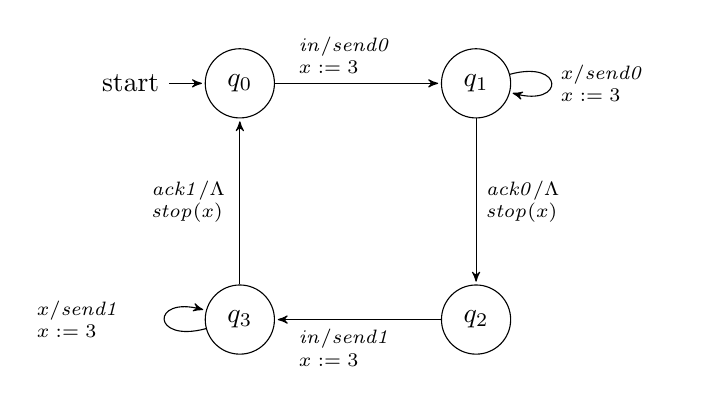
\begin{tikzpicture}[->,>=stealth',shorten >=1pt,auto,node distance=3cm,main node/.style={circle,draw,font=\sffamily\large\bfseries}]
  \node[initial, state] (1) {$q_0$};
  \node[state] (2) [right of=1] {$q_1$};
  \node[state] (3) [below of=2] {$q_2$};
  \node[state] (4) [below of=1] {$q_3$};

  \path[every node/.style={font=\sffamily\scriptsize}]
    (1) edge [text width=1.5cm] node {$\mathit{in}/\mathit{send0}$ \\ $x := 3$} (2)
    (2) edge [text width=1.5cm] node {$\mathit{ack0}/\Lambda$ \\ $\mathit{stop}(x)$} (3)
        edge [loop right, text width=1.5cm] node {$\toevent{x}/\mathit{send0}$\\ $x := 3$ } (2)
    (3) edge [text width=1.5cm] node {$\mathit{in}/\mathit{send1}$ \\ $x := 3$} (4)
    (4) edge [text width=1cm] node {$\mathit{ack1}/\Lambda$ \\ $\mathit{stop}(x)$} (1)
        edge [loop left, text width=1.5cm] node {$\toevent{x}/\mathit{send1}$\\ $x := 3$} (4);
\end{tikzpicture}
\caption{Mealy machine with a timer for alternating-bit protocol sender}
\label{fig:abp}
\end{figure}
In the diagram we write $x :=3$ to denote that a transition (re)starts a timer $x$ with value $3$,
and we write $\mathit{stop}(x)$ if s transition stops timer $x$.
For readability we have omitted trivial self-loops.
\iflong
$\Lambda$ denotes the absence of an observable output. 

In the model, input $\mathit{in}$ corresponds to a request from the upper layer to transmit data.
Initially, upon receipt of such a request, the sender builds a packet from the data and a sequence number $0$,
sends the packet over the network (output $\mathit{send0}$), and starts the timer with timeout value $3$.
If the sender receives an acknowledgement with the right sequence number $0$ (input $\mathit{ack0}$) 
then it stops the timer and jumps to state $q_2$.
Acknowledgement with the incorrect sequence number (input $\mathit{ack1}$) are ignored.
If no $\mathit{ack0}$ input arrives within $3$ timeunits, a timeout occurs and the same packet is sent again.
The behavior in states $q_2$ and state $q_3$ is analogous to that in states $q_0$ and $q_1$, respectively,
with the roles of $0$ and $1$ swapped.
\fi

The remainder of this article is structured as follows.
In Section 2, we present the formal definition of MMTs and their timed semantics.
Our timed semantics records at which (real) times inputs and outputs may occur, but we cannot observe whether some timer is started
in response to an input. Since we assume that a timeout immediately triggers an observable output, we may observe
(indirectly) the occurrence of a timeout, but we cannot observe which timer times out.
In Section 3, we present a surprising result, namely that under certain assumptions the timed semantics is equivalent to an untimed
semantics in which we can infer, for each timeout event, which previous event caused this timeout.
Intuitively, causality of timeouts can be inferred since a slight change in the timing of an input event leads to a corresponding slight change in
the timing of any timeouts that it induces.
Section 4, we use some basic concepts from the theory of timed automata (zones and DBMs) to show how we can compute the set of timers that may
timeout following some untimed run.
Section 5 presents our learning algorithm for MMTs. The equivalence of the timed and the untimed semantics allows us to prove
a Myhill-Nerode theorem for MMTs, which provides the basis for our learning algorithm. Our algorithm uses a learning algorithm for
(untimed) Mealy machines as a subroutine.
Section 6 contains some concluding remarks and lists topics for future research.


\section{Mealy machines with timers}

\subsection{Definition and timed semantics}
We assume an infinite set $X = \{ x_1, x_2, x_3,\ldots \}$ of {\em timers}.
Let $\toevents$ be the set of {\em timeout events} of the form
$\toevent{x}$ for $x \in X$.
For a set $I$, let $\extinputs$ be $I \cup \toevents$.
%
We write $A \hookrightarrow B$ for the set of partial functions from $A$ to $B$.
With $f \lceil A$ we denote the restriction of function $f$ to $\domof{f} \cap A$.
%For arbitrary functions $f$ and $g$, $f [g]$ is the function with domain $\domof{f}$ that behaves like $f$
%on $\domof{f} \setminus \domof{g}$ and like $g$ on $\domof{f} \cap \domof{g}$.
We write $\finitesubsets{A}$ for the set of finite subsets of set $A$.

\begin{definition}
\label{def:MMT}
A \emph{Mealy machine with timers (MMT)} is a tuple
\\
$\M = (I, O, Q, q_0, \vars, \delta, \lambda, \remap)$, where
\begin{itemize}
\item
$I$ and $O$ are finite sets of input events and output events, respectively,
\item
$Q$ is a finite set of states,
with
$q_0 \in Q$ the initial state,
\item
$\vars: Q \rightarrow \finitesubsets{X}$, with $\varsof{q_0} = \emptyset$,
\item
$\delta: Q \times \extinputs \hookrightarrow  Q$ is a transition function,
%with $\delta(q,i)$ defined iff $q \in Q$ and $i \in I \cup \{ \toevent{x} \mid x \in \varsof{q} \}$, 
\item
$\lambda: Q \times \extinputs \hookrightarrow O$ is an output function, 
\item
$\remap : Q \times \extinputs \hookrightarrow (X \hookrightarrow \natplus)$ is a timer update function.
\end{itemize}
Let $q \in Q$, $i \in \extinputs$, $q'=\delta(q,i)$ and $\rho=\remap(q,i)$. 
We require that $\varsof{q'} \setminus \varsof{q} \subseteq \domof{\rho} \subseteq\varsof{q'}$. 
When timer $x$ expires it is either stopped or restarted:
if $i=\toevent{x}$, for some $x$, then $x \not\in \varsof{q'} \setminus \domof{\rho}$.
%
We also require that input events are always enabled and timeout events are enabled
for timers that are active in the current state:
$\delta(q,i)$, $\lambda(q,i)$ and $\pi(q,i)$ are defined iff either
$i \in I$ or $i=\toevent{x}$, for some $x \in\varsof{q}$.
We write $q \xrightarrow{i/o,\rho} q'$ if $\delta(q,i) = q'$, $\lambda(q,i)= o$ and $\remap(q,i) = \rho$.
\end{definition}
Update function $\remap$ determines how timers are affected when an event occurs. Suppose $q \xrightarrow{i/o,\rho} q'$.
Basically, four things may happen:
%\marginpar{Add Venn diagram to illustrate situation?}
%Let $q \in Q$, $i \in \extinputs$, $\delta(q,i)=q'$ and $\remap(q,i)=\rho$.
\begin{enumerate}
\item
If $x \in\varsof{q} \setminus \varsof{q'}$ then input $i$ \emph{stops} timer $x$.
\item
If $x \in \varsof{q'} \setminus \varsof{q}$ then $i$ \emph{starts} timer $x$ with value $\rho(x)$.
\item
If $x \in \varsof{q} \cap \domof{\rho}$ then $i$ \emph{restarts} timer $x$ with value $\rho(x)$.
\item
Finally, if $x \in \varsof{q'} \setminus \domof{\rho}$ then timer $x$ is \emph{unaffected} by $i$.
\end{enumerate}

\paragraph{Semantics.}
The semantics of MMT $\M = (I, O, Q, q_0, \vars, \delta, \lambda, \remap)$ is defined via an infinite state transition system that describes all possible
configurations and transitions between them.
A \emph{valuation} is a partial function
$\tvals : X \hookrightarrow \realsplus$, defined on a finite subset of $X$, that assigns nonnegative real numbers as values to timers.
We write $\Vals{Y}$ for the set of valuations with domain $Y \subseteq X$.
A \emph{configuration} of an MMT is a pair $(q,\tvals)$, where $q \in Q$ is a state and $\tvals\in\Vals{\varsof{q}}$ is a valuation.
The \emph{initial configuration} is the pair $(q_0, \tvals_0)$, where $\tvals_0$ is the empty function.
Valuations and configurations can be modified by the occurrence of input and timeout events, and by
the occurrence of delays.
If $\tvals$ is a valuation in which all timers
have a value of at least $d$, then $d$ units of time may pass. As a result of this delay the value of all the timers is decremented by $d$.
Formally, for $\tvals, \tvals'$ valuations and $d \in \delays$, we define a delay transition relation by
\begin{eqnarray*}
\tvals \xrightarrow{d} \tvals' & \Leftrightarrow & [\domof{\tvals} = \domof{\tvals'} \wedge \forall x \in\domof{\tvals} : \tvals'(x) = \tvals(x) - d ].
\end{eqnarray*}
If the current valuation is $\tvals$, then timeout event $\toevent{x}$ may occur only if $\tvals(x)=0$.
If an input or a timeout event occurs, $\tvals$ is updated as specified by update function $\rho$.
The values of timers that are not affected by $\rho$ remain unchanged.
Formally, for $\tvals, \tvals'$ valuations, $i \in \extinputs$, $o \in O$ and $\rho \in X \hookrightarrow \natplus$,
we define a discrete transition relation by
\begin{eqnarray*}
\tvals \xrightarrow{i/o, \rho}  \tvals' & \Leftrightarrow & [ \domof{\tvals'} \setminus \domof{\tvals}  \subseteq \domof{\rho} \subseteq \domof{\tvals'} ~ \wedge\\
&& [\forall x \in\domof{\tvals'} : \tvals'(x) = \mbox{ if } x \in\domof{\rho} \mbox{ then } \rho(x) \mbox{ else } \tvals(x)] ~ \wedge\\
%More concise but harder to understand:
%&& \tvals' =  \tvals'[\tvals][\rho] ~ \wedge \\
&& \forall x \in X : i=\toevent{x} \Rightarrow (\tvals(x) = 0 \wedge x \not\in\domof{\tvals'} \setminus \domof{\rho})].
\end{eqnarray*}
%Condition $\tvals' =  \tvals'[\tvals][\rho]$ expresses that $\tvals'$ is obtained by giving variables
%in $\domof{\rho}$ the value specified by $\rho$, and all remaining variables the value specified by $\tvals$.
Transition relations $\xrightarrow{d}$ and $\xrightarrow{i/o, \rho}$ can be easily lifted to configurations.
For all configurations $(q, \tvals)$, $(q', \tvals')$ of an MMT $\M$,
\[
\frac{q = q' \quad \tvals \xrightarrow{d} \tvals'}{(q,\tvals) \xrightarrow{d} (q',\tvals')}
\quad\quad
  \frac{q \xrightarrow{i/o,\remapinst} q' \quad \tvals \xrightarrow{i/o, \rho} \tvals'}{(q,\tvals) \xrightarrow{i/o} (q',\tvals')}
\]
A \emph{timed run} of $\M$ over $w$ is a sequence 
\begin{eqnarray*}
\alpha & = & C_0 \xrightarrow{d_1} C'_0 \xrightarrow{i_1/o_1} C_1 \xrightarrow{d_2} C'_1 \xrightarrow{i_2/o_2} C_2 \cdots
\xrightarrow{d_k} C'_{k-1} \xrightarrow{i_k/o_k} C_{k}
\end{eqnarray*}
of transitions between configurations $C_j, C'_j$ of $\M$, where $C_0$ is the initial configuration.
%Note that, since MMTs are deterministic (if we allow to observe the
%identities of timers in timeout events),
%for each timed word $w$ there exists at most one run over $w$.
A \emph{timed word} over inputs $I$ and outputs $O$ is a sequence
\begin{eqnarray*}
w & = &  d_1 ~ i_1 ~ o_1 ~ d_2 ~ i_2 ~ o_2 \cdots d_k ~ i_k ~ o_k,
\end{eqnarray*}
where $d_j \in \delays$, $i_j \in I \cup \{ \mathit{to} \}$, and $o_j \in O$.
To each timed run $\alpha$ we associate a \emph{timed word} by forgetting the configurations and the timers
in timeout events:
\begin{eqnarray*}
\timedword(\alpha) & = & d_1 ~ i'_1 ~ o_1 ~ d_2 ~ i'_2 ~ o_2 \cdots d_k ~ i'_k ~ o_k, \mbox{ where for all } j,
i'_j  =  \left\{ \begin{array}{ll}
i_j & \mbox{if } i_j \in I,\\
\mathit{to} & \mbox{if } i_j \in \toevents.
\end{array} \right.
\end{eqnarray*}
The idea is that timeouts cannot be observed directly. 
However, when we observe an output that is not triggered by an input, we may
conclude that a timeout occurred. But in general we do not know which timer expired.

We say $w$ is a timed word of $\M$ if $\M$ has a timed run $\alpha$ with $w = \timedword(\alpha)$.
%
Two MMTs $\M$ and $\N$ with the same sets of inputs are \emph{timed equivalent}, denoted $\M \approx_{\mathit{timed}} \N$, iff 
they have the same sets of timed words.

\iflong
\paragraph{Remark.}
In our semantics we assume that discrete transitions occur instantaneously and take no time. In applications, however, i/o interactions
often take a significant amount of time. In \cite{SHV16}, for instance, a case study of an interventional X-ray system is
described in which a single i/o interaction may take several seconds. If it is important to model such delays
explicitly, this can be done within the MMT framework by splitting a transition with input $i$ and output $o$ into
a pair of consecutive transitions: a first transition with input $i$ and some default output $\Lambda$ that starts
a timer $x$, and a second transition in which $x$ times out and output $o$ is produced.
If inputs arrive in the newly introduced intermediate state, these may either be ignored, buffered or forbidden
(via a transition to some designated error state).
Note that $\Lambda$ corresponds to the \emph{absence} of an observable output. For inputs $i \in I$ this is fine: if such
an input does not trigger an observable output then we just assume that the output event is $\Lambda$. We do not allow
$\Lambda$ as output event in timeout transitions $\toevent{x}$: since timeout events themselves are not observable, we can ony observe their occurrence indirectly through the observable output that they trigger.

\paragraph{Remark.}
Note that we assume that in a timed run each discrete transition is preceded by a nonzero delay.
The idea that multiple consecutive discrete transitions may occur in zero time is a useful abstraction in synchronous
programming and in the theory of timed automata, but nonzero delays form
a crucial requirement for the learning algorithm that we present in this paper.

Disallowing zero delays creates certain complications that we have to deal with. The simple MMT of Figure~\ref{fig:timelock}, for instance,
may reach a timelock following the timed word $1 ~ i ~ o ~ 1 ~ i ~ o$: at this point timer $x$ has value $0$, but no timeout is enabled since first a nonzero amount of time has to elapse, which is not possible since then $x$ would become negative.
\begin{figure}[ht]
\begin{center}
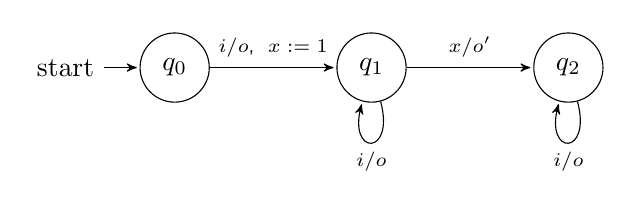
\begin{tikzpicture}[->,>=stealth',shorten >=1pt,auto,node distance=2.5cm,main node/.style={circle,draw,font=\sffamily\large\bfseries}]
  \node[initial, state] (1) {$q_0$};
  \node[state] (2) [right of=1] {$q_1$};
  \node[state] (3) [right of=2] {$q_2$};
  
  \path[every node/.style={font=\sffamily\scriptsize}]
    (1) edge node {$i/o$, $~x:=1$} (2)  
    (2) edge  node {$\toevent{x}/o'$} (3)
        edge  [loop below] node {$i/o$} (2)
    (3) edge  [loop below] node {$i/o$} (4);
\end{tikzpicture}
\caption{An MMT with a timelock}
\label{fig:timelock}
\end{center}
\end{figure}
Once solution would be to disable inputs in $I$ whenever a timer has become $0$. 
In Section~\ref{section untimed semantics}, we will elaborate
a different approach in which we only consider runs in which no ``races'' occur. This eliminates the problematic
behavior of the above MMT in which there is a race between the second $i$ event and the timeout.
\fi

\paragraph{Nondeterminism.}
Due to our assumption that we cannot observe the identity of a timer in a timeout event, an MMT may exhibit nondeterministic
behavior: even if we offer exactly the same inputs at exactly the same time, different outputs may occur in different runs. 
The MMT of Figure~\ref{fig:nondeterminism} (left), for instance, accepts both the timed words
$1 ~ i ~ o ~ 1 ~ \mathit{to} ~ o'$ and $1 ~ i ~ o ~ 1 ~ \mathit{to} ~ o''$.
(For clarity, we omit some self-loop transitions.)
\begin{figure}[ht]
\vspace{-2em}
\begin{center}
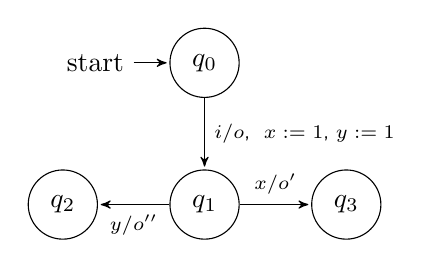
\begin{tikzpicture}[->,>=stealth',shorten >=1pt,auto,node distance=1.8cm,main node/.style={circle,draw,font=\sffamily\large\bfsthe name of the eries}]
  \node[initial, state] (1) {$q_0$};
  \node[state] (2) [below of=1] {$q_1$};
  \node[state] (3) [right of=2] {$q_3$};
  \node[state] (4) [left of=2] {$q_2$};

  \path[every node/.style={font=\sffamily\scriptsize}]
    (1) edge node {$i/o$, $~x:=1$, $y:=1$} (2)  
    (2) edge  node {$\toevent{x}/o'$} (3)
     edge  node {$\toevent{y}/o''$} (4);
\end{tikzpicture}
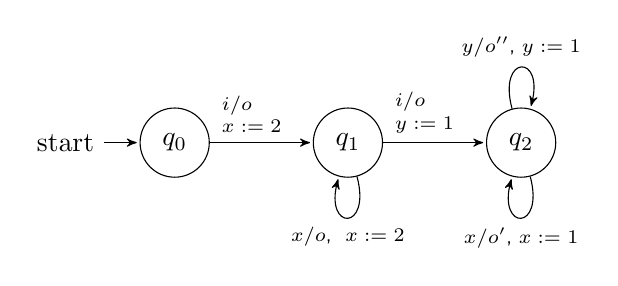
\begin{tikzpicture}[->,>=stealth',shorten >=1pt,auto,node distance=2.2cm,main node/.style={circle,draw,font=\sffamily\large\bfseries}]
  \node[initial, state] (1) {$q_0$};
  \node[state] (2) [right of=1] {$q_1$};
  \node[state] (3) [right of=2] {$q_2$};

  \path[every node/.style={font=\sffamily\scriptsize}]
    (1) edge [text width=1cm] node {$i/o$\\ $x:=2$} (2)  
    (2) edge [text width=1cm] node {$i/o$\\ $y:=1$} (3)
      edge  [loop below] node {$\toevent{x}/o$, $~x:=2$} (2)
   (3) edge  [loop below] node {$\toevent{x}/o'$, $x:=1$} (3)
   edge  [loop above] node {$\toevent{y}/o''$, $y:=1$} (3);
\end{tikzpicture}
\caption{MMTs with ``uncontrollable'' and ``controllable'' nondeterminism}
\label{fig:nondeterminism}
\end{center}
\end{figure}

%In order to rule out this type of nondeterminism, it is not enough to require that the timer update functions are injective,
%that is, it is not allowed to assign the same value to multiple timers in a single transition.
%This is illustrated by the MMT of Figure~\ref{fig:nondeterminism2}, which accepts both the timed words
%$1 ~ i ~ o ~ 1 ~ \mathit{to} ~ o'~ 1 ~ \mathit{to} ~ o'$ and $1 ~ i ~ o ~ 1 ~ \mathit{to} ~ o' ~ 1 ~ \mathit{to} ~ o''$.
%\begin{figure}[ht]
%\begin{center}
%\begin{tikzpicture}[->,>=stealth',shorten >=1pt,auto,node distance=2.5cm,main node/.style={circle,draw,font=\sffamily\large\bfseries}]
%  \node[initial, state] (1) {$q_0$};
%  \node[state] (2) [below of=1] {$q_1$};
%  \node[state] (4) [left of=2] {$q_2$};
%
%  \path[every node/.style={font=\sffamily\scriptsize}]
%    (1) edge node {$i/o$, $~x:=1$, $y:=2$} (2)  
%    (2) edge  node {$\toevent{y}/o''$} (4)
%      edge  [loop right] node {$\toevent{x}/o'$, $~x:=1$} (2);
%\end{tikzpicture}
%\caption{Another MMT with nondeterministic behavior}
%\label{fig:nondeterminism2}
%\end{center}
%\end{figure}
%
The nondeterminism of the MMT of Figure~\ref{fig:nondeterminism} (left)
%and \ref{fig:nondeterminism2} 
is ``uncontrollable'' and occurs after any (nonempty) input sequence.
Figure~\ref{fig:nondeterminism} (right) gives an example of an MMT that exhibits nondeterminism when the second input occurs \emph{exactly} one time unit after the first input: the MMT accepts timed words
$7 ~ i ~ o ~ 1 ~ i ~ o ~ 1 ~ \mathit{to} ~ o'$ and $7 ~ i ~ o ~ 1 ~ i ~ o ~ 1 ~ \mathit{to} ~ o''$.
This type of nondeterminism is ``controllable'' and will not occur if we carefully
select the timing of inputs.


\subsection{Timed and untimed runs and behaviors}
Configurations consists of pairs of states and timer valuations. This means that there are two natural abstractions of
timed runs: an abstraction $\untime$ that forgets all timing information and keeps the transitions of the MMT, 
and an abstraction $\beh$ that forgets information on states and preserves the timing information.
When we compose these abstractions we obtain \emph{untimed behaviors} in which only information about inputs, outputs,
updates and active timers is preserved.
The abstractions commute, $\beh(\untime(\alpha))=\untime(\beh(\alpha))$, and play a key role in
the technical development of this paper.
%
Formally, an \emph{untimed behavior} over inputs $I$ and outputs $O$ is a sequence 
\begin{eqnarray*}
\beta & = & X_0 \xrightarrow{i_1/o_1, \rho_1} X_1  \xrightarrow{i_2/o_2, \rho_2} X_2 \cdots \xrightarrow{i_k/o_k, \rho_k} X_{k},
\end{eqnarray*}
where $X_0 \subseteq X$ and, for each $j>0$,  $i_j \in \extinputs$, $o_j \in O$, $\rho_j \in X \hookrightarrow \natplus$, and
 $X_j \setminus X_{j-1}  \subseteq \domof{\rho_j} \subseteq X_j \subseteq X$.
Moreover, if $i_j = \toevent{x}$, for some $j>0$, then $x \in X_{j-1}$ and $x \not\in X_j \setminus \domof{\rho_j}$.
%
An \emph{untimed run} of an MMT $\M$ is a sequence
\begin{eqnarray*}
\gamma & = & q_0 \xrightarrow{i_1/o_1, \rho_1} q_1  \xrightarrow{i_2/o_2, \rho_2} q_2 \cdots \xrightarrow{i_k/o_k, \rho_k} q_k
\end{eqnarray*}
of transitions of $\M$ that starts with the initial state $q_0$. 
To each untimed run $\gamma$ we associate an untimed behavior by replacing all
states by their sets of timers:
\begin{eqnarray*}
\beh(\gamma) & = & \vars(q_0) \xrightarrow{i_1/o_1, \rho_1} \vars(q_1)  \xrightarrow{i_2/o_2, \rho_2} \vars(q_2) \cdots \xrightarrow{i_k/o_k, \rho_k} \vars(q_k).
\end{eqnarray*}
We say that $\beta$ is an untimed behavior of $\M$ if $\M$ has an untimed run $\gamma$ with $\beh(\gamma) = \beta$.
Note that the initial timer set of an untimed behavior of $\M$ is empty.
%
A \emph{timed behavior} over inputs $I$ and outputs $O$ is an alternating sequence
\begin{eqnarray}
\label{timedbehavior}
\sigma & = & \tvals_0 \xrightarrow{d_1} \tvals'_0 \xrightarrow{i_1/o_1, \rho_1} \tvals_1 \xrightarrow{d_2} \tvals'_1 \xrightarrow{i_2/o_2, \rho_2} \tvals_2 \cdots
\xrightarrow{d_k} \tvals'_{k-1} \xrightarrow{i_k/o_k, \rho_k} \tvals_{k}
\end{eqnarray}
of delay transitions and discrete transitions with, for each $j$,
$\tvals_j, \tvals'_j$ valuations and,
for each $j>0$,  $d_j \in \delays$, $i_j \in \extinputs$, $o_j \in O$, and $\rho_j \in X \hookrightarrow \natplus$.
To each timed behavior $\sigma$ we associate an untimed behavior by forgetting the
delays transitions and by replacing valuations by their domain:
\begin{eqnarray*}
\untime(\sigma) & = & \domof{\tvals_0} \xrightarrow{i_1/o_1, \rho_1} \domof{\tvals_1}  \xrightarrow{i_2/o_2, \rho_2} \domof{\tvals_2} \cdots \xrightarrow{i_k/o_k, \rho_k} \domof{\tvals_k}.
\end{eqnarray*}
We say that untimed behavior $\beta$ is \emph{feasible} if there exists a timed behavior $\sigma$ such that $\untime(\sigma) = \beta$.
We also associate a timed word to timed behavior $\sigma$ by forgetting valuations, timers, and update functions:
\begin{eqnarray*}
\timedword(\sigma) & = & d_ 1 ~ i'_1 ~ o_1 ~ i'_2 ~ o_2 \cdots d_k ~ i'_k ~ o_k, \mbox{ where for all } j,
i'_j  =  \left\{ \begin{array}{ll}
i_j & \mbox{if } i_j \in I,\\
\mathit{to} & \mbox{if } i_j \in \toevents.
\end{array} \right.
\end{eqnarray*} 
Let $\alpha$ be a timed run of an MMT $\M$: 
\begin{eqnarray*}
\alpha & = & (q_0, \tvals_0) \xrightarrow{d_1} (q_0, \tvals'_0) \xrightarrow{i_1/o_1} (q_1, \tvals_1) \xrightarrow{d_2} (q_1, \tvals'_1)  \cdots
 \xrightarrow{i_k/o_k} (q_k, \tvals_k).
\end{eqnarray*}
Then $\alpha$ can be projected both to an untimed run of $\M$
\begin{eqnarray*}
\untime (\alpha) & = & q_0 \xrightarrow{i_1/o_1, \rho_1} q_1  \xrightarrow{i_2/o_2, \rho_2} q_2 \cdots \xrightarrow{i_k/o_k, \rho_k} q_k
\end{eqnarray*}
(the $\rho_j$'s are determined since $\M$ is deterministic) and to a timed behavior
\begin{eqnarray*}
\beh(\alpha) & = & \tvals_0 \xrightarrow{d_1} \tvals'_0 \xrightarrow{i_1/o_1, \rho_1} \tvals_1 \xrightarrow{d_2} \tvals'_1 \xrightarrow{i_2/o_2, \rho_2} \tvals_2 \cdots
\xrightarrow{d_k} \tvals'_{k-1} \xrightarrow{i_k/o_k, \rho_k} \tvals_{k}.
\end{eqnarray*}
\iflong
We say that $\sigma$ is an timed behavior of $\M$ if $\M$ has an timed run $\alpha$ with $\beh(\alpha) = \sigma$.
\fi
Note that $\beh(\untime(\alpha))=\untime(\beh(\alpha))$ and $\timedword(\alpha) = \timedword(\beh(\alpha))$.
\iflong
Thus the diagram of Figure~\ref{fig:diagram}, which summarizes the various types of runs and behaviors that we consider
in this article, commutes.
\begin{figure}[h]
\centering
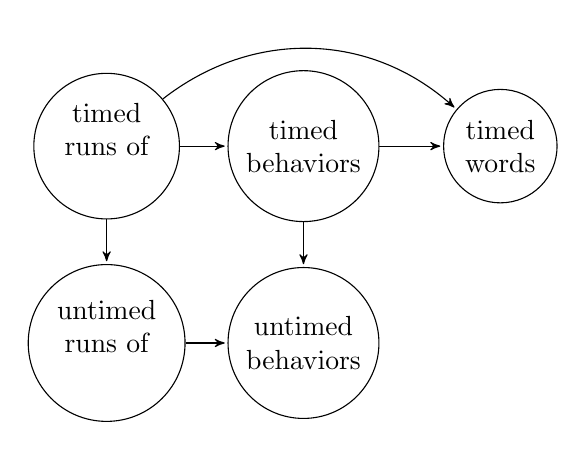
\begin{tikzpicture}[->,>=stealth',shorten >=1pt,auto,node distance=2.5cm,main node/.style={circle,draw,font=\sffamily\large\bfseries}]
  \node[state,align=center] (1) {timed \\ runs of\\ $\M$};
  \node[state,align=center] (2) [below of=1] {untimed \\ runs of\\ $\M$};
  \node[state,align=center] (3) [right of=1] {timed\\ behaviors};
  \node[state,align=center] (4) [right of=2] {untimed\\ behaviors};
  \node[state,align=center] (5) [right of=3] {timed \\words};

  \path[every node/.style={font=\sffamily\scriptsize}]
    (1) edge  node {$\untime$} (2)
        edge  node {$\beh$} (3)
        edge[bend left=40]  node {$\timedword$} (5)
    (2) edge  node {$\beh$} (4)
    (3) edge  node {$\untime$} (4)
        edge  node {$\timedword$} (5);
\end{tikzpicture}
\caption{Functions relating different types of runs and behaviors}
\label{fig:diagram}
\end{figure}
\fi
Conversely, if $\gamma$ is an untimed run  of $\M$ and $\sigma$ is a timed behavior such that $\beh(\gamma) = \untime(\sigma)$,
then there exists a unique timed run $\alpha$ of $\M$ with $\untime(\alpha) = \gamma$ and $\beh(\alpha) = \sigma$.
We refer to $\alpha$ as $\run(\gamma,\sigma)$.

For any nonempty sequence $\sigma$, $\Head{\sigma}$ denotes the first element, $\Tail{\sigma}$ denotes the sequence obtained by removing the first element, and $\Last{\sigma}$ denotes the last element.
Suppose $\beta, \beta'$ are untimed behaviors over $I$ and $O$ such that $\Last{\beta} = \Head{\beta'}$.
Then the \emph{sequential composition} of $\beta$ and $\beta'$, written $\beta \cdot \beta'$, is the untimed behavior $\beta ~ \Tail{\beta'}$.
Behavior $\beta$ is a \emph{prefix} of behavior $\gamma$ if there exists an behavior $\beta'$ such that $\gamma = \beta \cdot \beta'$.

\section{Untimed semantics}
\label{section untimed semantics}
We would, intuitively, like to define the untimed semantics of an MMT $\M$ as the set of its feasible untimed behaviors.
However, this semantics would then depend heavily on the identity of the timers. Therefore, we define an equivalence relation
on untimed behaviors, which deems two untimed behaviors equivalent if there is a consistent renaming of timers that transforms
the one into the other.

Let $\beta$ and $\beta'$ be two untimed behaviors with the same length and outputs:
\begin{eqnarray*}
\beta & = & X_0 \xrightarrow{i_1/o_1, \rho_1} X_1  \xrightarrow{i_2/o_2, \rho_2} X_2 \cdots \xrightarrow{i_k/o_k, \rho_k} X_{k},\\
\beta' & = & Y_0 \xrightarrow{i'_1/o_1, \rho'_1} Y_1  \xrightarrow{i'_2/o_2, \rho'_2} Y_2 \cdots \xrightarrow{i'_k/o_k, \rho'_k} Y_{k}.
\end{eqnarray*}
An \emph{isomorphism} from $\beta$ to $\beta'$ is a list $f = f_0 ,\ldots, f_k$ of bijections $f_j : X_j \rightarrow Y_j$ such that
for all $j>0$: (1) for all $x \in X_j \setminus \domof{\rho_j})$, $f_j(x)=f_{j-1}(x)$,
(2) $i'_j = i_j$ if $i_j \in I$ and $i'_j = \toevent{f_{j-1}(x)}$ if $i_j = \toevent{x}$, for some $x \in X_{j-1}$, and
(3) $\domof{\rho'_j} = f_j(\domof{\rho_j})$ and $\rho'_j(y) = \rho_j ( f_j^{-1}(y))$, for all $y\in\domof{\rho'_j}$.
In this case, since $\beta'$ is fully determined by $\beta$ and $f$, we write $\beta' = f(\beta)$.
We say that $\beta$ and $\beta'$ are \emph{isomorphic} if there exists an isomorphism $f$ from $\beta$ to $\beta'$.
Two sets of untimed behaviors $A$ and $B$ are \emph{isomorphic} if for each untimed behavior of $A$ there is an isomorphic untimed behavior in $B$,
and vice versa.
\iflong

Isomorphisms can be lifted to timed behaviors in the obvious way. 
Let $\sigma$ and $\sigma'$ be two timed behaviors with the same length and outputs:
\begin{eqnarray*}
\sigma & = & \tvals_0 \xrightarrow{d_1} \tvals'_0 \xrightarrow{i_1/o_1, \rho_1} \tvals_1  \cdots
\xrightarrow{d_k} \tvals'_{k-1} \xrightarrow{i_k/o_k, \rho_k} \tvals_{k},\\
\sigma' & = & \lambda_0 \xrightarrow{d_1} \lambda'_0 \xrightarrow{i'_1/o_1, \rho'_1} \lambda_1  \cdots
\xrightarrow{d_k} \lambda'_{k-1} \xrightarrow{i'_k/o_k, \rho'_k} \lambda_{k}.
\end{eqnarray*}
An \emph{isomorphism} from $\sigma$ to $\sigma'$ is a list $f = f_0 ,\ldots, f_k$ of bijections such that
(1) $f$ is an isomorphism from $\untime(\sigma)$ to $\untime(\sigma')$, and
$\lambda_j = \kappa_j \circ f_j^{-1}$ and $\lambda'_j = \kappa'_j \circ f_j^{-1}$, for all $j$.
Since $\sigma'$ is fully determined by $\sigma$ and $f$, we write $\sigma' = f(\sigma)$.
Two timed behaviors $\sigma$ and $\sigma'$ are \emph{isomorphic} if there exists an isomorphism $f$ from $\sigma$ to $\sigma'$.
Since an isomorphism only renames timers, which do not appear in timed words, 
isomorphic timed behaviors induce identical timed words: $\sigma' = f(\sigma) \Rightarrow \timedword(\sigma') = \timedword(\sigma)$.

The following lemmas follow directly from the definitions:
\begin{lemma}
\label{lemma isomorphism}
Let $\sigma$ be a timed behavior and let $f$ be an isomorphism for $\sigma$.
Then $\untime(f(\sigma)) = f(\untime(\sigma))$.
\end{lemma}
\begin{lemma}
If untimed behaviors $\beta$ and $\beta'$ are isomorphic, then $\beta$ is feasible iff $\beta'$ is feasible.
\end{lemma}

\fi
Two MMTs $\M$ and $\N$ with the same sets of inputs are \emph{untimed equivalent}, denoted $\M \approx_{\mathit{untimed}} \N$, iff their sets of feasible untimed behaviors are isomorphic.
\iflong
Untimed equivalence is finer than timed equivalence.
\fi

\begin{theorem}
\label{untimedimpliestimed}
$\M \approx_{\mathit{untimed}} \N$
implies
$\M \approx_{\mathit{timed}} \N$.
\end{theorem}
\iflong
\begin{proof}
Assume $\M \approx_{\mathit{untimed}} \N$ and $w$ is a timed word of $\M$.
Since $\approx_{\mathit{timed}}$ is symmetric, it suffices to prove that $w$ is a timed word of $\N$.
Since $w$ is a timed word of $\M$,
there exists a timed run $\alpha$ of $\M$ with $\timedword(\alpha) = w$. 
Let $\sigma = \beh(\alpha)$ and $\beta = \untime(\sigma)$. 
Then $\beta$ is a feasible untimed behavior of $\M$ and $\timedword(\sigma) = w$.
Since  $\M \approx_{\mathit{untimed}} \N$, there exists an isomorphism $f$ such that 
$\beta' = f(\beta)$ is a feasible untimed behavior of $\N$.
Hence $\N$ has an untimed run $\gamma'$ such that $\untime(\gamma') = \beta'$.
Let $\sigma' = f(\sigma)$.
By Lemma~\ref{lemma isomorphism}, $\sigma'$ is a timed behavior with 
$\untime(\sigma') = \untime(f(\sigma)) = f(\untime(\sigma)) = f(\beta) = \beta'$.
Since $\beh(\gamma') = \untime(\sigma') = \beta'$, $\N$ has a timed run $\alpha' = \run(\gamma',\sigma')$ with
$\beh(\alpha') = \sigma'$.
Note that $\timedword(\alpha') = \timedword(\sigma') = \timedword(f(\sigma)) = \timedword(\sigma) = w$.
Hence $w$ is a timed word of $\N$, as required.
\end{proof}
\fi
The converse of Theorem~\ref{untimedimpliestimed} does not hold. 
The two MMTs of Figure~\ref{fig:twoequivalentone}, for instance,
are timed equivalent but not untimed equivalent,
because the top MMT has an untimed behavior
$ \emptyset \xrightarrow{i/o,~ x, y:=1,2 } \{ x, y \}$, for which the bottom MMT has no isomorphic behavior.
\begin{figure}
\ifshort
\vspace{-1em}
\fi
\begin{center}
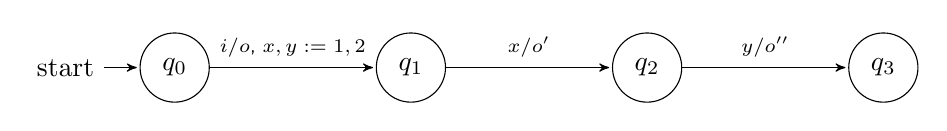
\begin{tikzpicture}[->,>=stealth',shorten >=1pt,auto,node distance=3cm,main node/.style={circle,draw,font=\sffamily\large\bfseries}]
  \node[initial, state] (1) {$q_0$};
  \node[state] (2) [right of=1] {$q_1$};
  \node[state] (3) [right of=2] {$q_2$};
  \node[state] (4) [right of=3] {$q_3$};

  \path[every node/.style={font=\sffamily\scriptsize}]
    (1) edge node {$i/o$, $x, y:=1,2$} (2)  
    (2) edge  node {$\toevent{x}/o'$} (3)
   (3) edge node {$\toevent{y}/o''$} (4);
\end{tikzpicture}

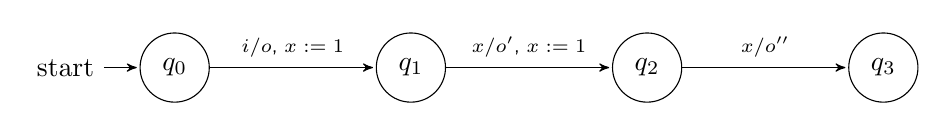
\begin{tikzpicture}[->,>=stealth',shorten >=1pt,auto,node distance=3cm,main node/.style={circle,draw,font=\sffamily\large\bfseries}]
  \node[initial, state] (1) {$q_0$};
  \node[state] (2) [right of=1] {$q_1$};
  \node[state] (3) [right of=2] {$q_2$};
  \node[state] (4) [right of=3] {$q_3$};

  \path[every node/.style={font=\sffamily\scriptsize}]
    (1) edge node {$i/o$, $x:=1$} (2)  
    (2) edge  node {$\toevent{x}/o'$, $x:=1$} (3)
   (3) edge node {$\toevent{x}/o''$} (4);
\end{tikzpicture}
\caption{Timed equivalent but not untimed equivalent}
\label{fig:twoequivalentone}
\end{center}
\end{figure}
For this reason, we restrict ourselves in the rest of this article to MMTs in which at most
one clock can be (re)set in a single transition. This restriction has the additional advantage that it
eliminates the uncontrollable nondeterminism illustrated in Figure~\ref{fig:nondeterminism}.
% and \ref{fig:nondeterminism2}.
Provided there is no uncontrollable nondeterminism, most MMTs
have an equivalent MMT that (re)sets at most one timer per transition:
if multiple timers are started simultaneously then we can often encode this by just
starting the timer $x$ with the smallest value $d_0$, and recording the set of remaining timers in the discrete state.
Then, when $x$ expires, we start the next timer (with timeout value decremented by $d_0$), etc.
However, such an encoding is not always possible. 
\iflong
Figure~\ref{fig:counterexample} presents an example of an MMT for which no equivalent MMT exists
in which at most one timer is (re)set per transition.
\begin{figure}
\begin{center}
\begin{tikzpicture}[->,>=stealth',shorten >=1pt,auto,node distance=2.7cm,main node/.style={circle,draw,font=\sffamily\large\bfseries}]
  \node[initial, state] (1) {$q_0$};
  \node[state] (2) [right of=1] {$q_1$};
  \node[state] (3) [right of=2] {$q_2$};
  \node[state] (4) [right of=3] {$q_3$};
  \node[state] (5) [below of=2] {$q_4$};

  \path[every node/.style={font=\sffamily\scriptsize}]
    (1) edge node {$i/o$, $x, y:=1,2$} (2)  
    (2) edge  node {$i/o$} (3)
   (3) edge node {$\toevent{y}/o''$} (4)
   (2) edge node {$\toevent{x}/o'$} (5);
\end{tikzpicture}
\caption{Starting more than one timer on a transition increases expressivity}
\label{fig:counterexample}
\end{center}
\end{figure}
\fi

Even when we restrict to MMTs that may (re)set at most one timer per transition, there is a difference
between the timed and the untimed semantics.
This is due to the fact that an MMT may have timers that are always stopped or restarted before
they expire. Such ``ghost'' timers are visible in the untimed semantics but cannot be observed in the timed semantics.
\iflong
Figure~\ref{fig:ghosttimers} gives an example of an MMT with a ghost timer. The MMT is equivalent to the MMT obtained by 
omitting the update $y :=60$ on the transition from $q_1$ to $q_2$.
\begin{figure}
\begin{center}
\begin{tikzpicture}[->,>=stealth',shorten >=1pt,auto,node distance=2.7cm,main node/.style={circle,draw,font=\sffamily\large\bfseries}]
  \node[initial, state] (1) {$q_0$};
  \node[state] (2) [right of=1] {$q_1$};
  \node[state] (3) [right of=2] {$q_2$};
  \node[state] (4) [right of=3] {$q_3$};
  \node[state] (5) [below of=2] {$q_4$};

  \path[every node/.style={font=\sffamily\scriptsize}]
    (1) edge node {$i/o$, $x:=1$} (2)  
    (2) edge  node {$i/o$, $y:=60$} (3)
   (3) edge node {$\toevent{x}/o''$} (4)
   (2) edge node {$\toevent{x}/o'$} (5);
\end{tikzpicture}
\caption{MMT with ghost timer $y$}
\label{fig:ghosttimers}
\end{center}
\end{figure}
\fi
%Let $\M$ be an MMT. Then we say that $\M$ is \emph{timer live} if, for each time run $\alpha$ and for each timer $x$
%\marginpar{How can we decide timer liveness?}
%of the final configuration of $\alpha$, there exists an extension $\alpha'$ of $\alpha$ in which timer $x$ 
%remains unaffected until it expires.
%
We say that an MMT $\M$ is \emph{timer live} if, for each feasible untimed behavior $\beta$ and for each timer $y$ that is running after $\beta$, there exists an untimed behavior $\beta_y$ consisting of transitions that leave $y$ unaffected, except for the last one in which $y$ expires, and such that $\beta \cdot \beta_y$ is feasible.
\iflong
Clearly, the MMT of Figure~\ref{fig:ghosttimers} is not timer live, as there is no way to extend the feasible untimed
behavior $\emptyset \xrightarrow{i/o,~ x:=1 } \{ x\} \xrightarrow{i/o,~ y:=60 } \{ x, y\}$ to an untimed behavior in which
timer $y$ expires.
\fi

We will show that the timed semantics and the untimed semantics coincide for timer live MMTs in which at most one timer is (re)started on each transition. However, in order prove this result we need to do some prepatory work.

\paragraph{Wiggling.}
Often it is possible to slightly change the timing of events in a timed behavior, 
while preserving the associated untimed behavior.
\iflong
Consider, for instance, a timed behavior 
\[
\tvals_0 \xrightarrow{d_1} \tvals'_0 \xrightarrow{i_1/o_1, \rho_1} \tvals_1 \cdots
\xrightarrow{d_j} \tvals'_{j-1} \xrightarrow{i_j/o_j, \rho_j} \tvals_j  \xrightarrow{d_{j+1}} \cdots
\xrightarrow{d_k} \tvals'_{k-1} \xrightarrow{i_k/o_k, \rho_k} \tvals_{k}
\]
that contains an $i_j$-transition that is not a timeout and does not (re)start any timer.
We can then schedule this transition slightly earlier.
More precisely, if $0 < e < d_j$ and $e' = d_j + d_{j+1}- e $ then we can find $\tvals, \tvals'$ such that
\[
\tvals_0 \xrightarrow{d_1} \tvals'_0 \xrightarrow{i_1/o_1, \rho_1} \tvals_1 \cdots
\xrightarrow{e} \tvals' \xrightarrow{i_j/o_j, \rho_j} \tvals  \xrightarrow{e'} \cdots
\xrightarrow{d_k} \tvals'_{k-1} \xrightarrow{i_k/o_k, \rho_k} \tvals_{k}
\]
is a timed behavior with the same underlying untimed behavior.

We may also be able to wiggle the timing of timeouts and transitions that (re)start a timer,
but here we have to be more careful.
\fi
If we shift the timing of an input event by a small amount then we must also shift the timing of a subsequent timeout
that is triggered by this input.
In addition, if the timeout starts another timer then we also need to shift the timeout event that this timer induces, etc.
%
Let us formalize these ideas. Consider a timed behavior $\sigma$ as in equation (\ref{timedbehavior})
with events $i_p$ and $i_q$ with $p < q$.
Then we say that $i_p$ \emph{triggers} $i_q$ if there exists a timer $x$ such that:
(a) event $i_p$ starts $x$, 
(b) for all $p < r < q$, $x$ is unaffected by event $i_r$, and
(c) $i_q = \toevent{x}$.
A \emph{block} of $\sigma$ is a maximal subset of indices $B = \{ p_1 ,\ldots, p_u \}$ such that $i_{p_1}$ triggers $i_{p_2}$, $i_{p_2}$ triggers $i_{p_3}$, etc.
Note that the collection of blocks of $\sigma$ partitions the set of indices $\{ 1 ,\ldots, k \}$.
We refer to this partition as $\Pi_{\sigma}$.
We say that timed behavior $\sigma$ contains a \emph{race} if there is some index $j>0$ and some timer $x$  
such that $\kappa'_{j-1}(x) = 0$ and $i_j \neq \toevent{x}$.
The following lemma allows us to shift all events in a block simultaneously forward or backward by a small amount, 
under the condition that there are no races.

\begin{lemma}
\label{wiggle lemma}
Suppose $\sigma$ is a timed behavior as in equation (\ref{timedbehavior}) without races.
Suppose $B = \{ p_1 ,\ldots, p_u \}$ is a block of $\sigma$, and suppose
that $\epsilon$ is a real number whose absolute is smaller than any nonzero number that occurs in $\sigma$, that is
$\mid \epsilon \mid  < \min (\bigcup_{1 \leq j \leq k} \{ d_j \} \cup \ranof{\kappa'_j} \setminus \{ 0 \} )$.
Then there exists a timed behavior
$\sigma'  =  \lambda_0 \xrightarrow{e_1} \lambda'_0 \xrightarrow{i_1/o_1, \rho_1} \lambda_1 \xrightarrow{e_2} \lambda'_1 \xrightarrow{i_2/o_2, \rho_2} \lambda_2 \cdots
\xrightarrow{e_k} \lambda'_{k-1} \xrightarrow{i_k/o_k, \rho_k} \lambda_{k}$
without races such that
$\untime(\sigma)=\untime(\sigma')$,
$\kappa_0 = \lambda_0$, and
$e_j  =  d_j + \epsilon  \mbox{ if } j-1 \not\in T \wedge j \in T$,
$e_j = d_j  \mbox{ if } j-1 \in T \Leftrightarrow j \in T$, and
$e_j = d_j - \epsilon  \mbox{ if } j-1 \in T \wedge j \not\in T$.
\end{lemma}
In the presence of races, Lemma~\ref{wiggle lemma} does not hold. 
Consider the following timed behavior with blocks $\{ 1, 3 \}$, $\{ 2 \}$,
\iflong 
and $\{ 4, 5 \}$, visualized in Figure~\ref{fig:races}:
\else
and $\{ 4, 5 \}$:
\fi
\[
\emptyset \xrightarrow{7} \emptyset \xrightarrow{i_1/o_1, x \mapsto 2} (x=2) \xrightarrow{1} (x=1)
\xrightarrow{i_2/o_2, y \mapsto 1} (x=y=1) \xrightarrow{1} (x=y=0) 
\]
\[
\xrightarrow{\toevent{x}/o_3, u \mapsto 2} (u=2)
\xrightarrow{1} (u=1)
\xrightarrow{i_4/o_4, z \mapsto 1} (u=z=1)
\xrightarrow{1} (u=z=0)\xrightarrow{\toevent{z}/o_5} (u=0).
\]

\iflong
\begin{figure}
\vspace{-2em}
\begin{center}
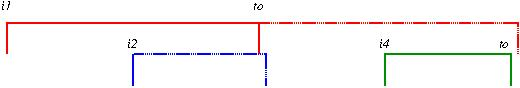
\includegraphics[width=.45\textwidth]{wiggling.jpg}
\end{center}
\caption{A timed behavior with two races}
\label{fig:races}
\end{figure}
\fi
This timed behavior contains two races, after two and four time units, respectively.
The first races is won by block $\{ 1, 3 \}$, and the second race is won by block $\{ 4, 5 \}$.
As a result of these races we cannot wiggle the timing of block $\{ 1, 3 \}$ by any amount:
if $i_1$ occurs just a bit later then timer $y$ must expire before timer $x$,
and if $i_1$ occurs just a bit earlier then timer $u$ must expire before timer $z$.
Note that when timer $x$ expires timer $y$ is stopped.
%
The above scenario is similar to the well-known Rush Hour puzzle game,
in which one has to slide blocking vehicles out of the way to find a path for one specific red car to exit a parking lot.
The next lemma asserts that we can always solve the puzzle for MMTs: for any timed behavior that contains races,
an equivalent timed behavior exists without races.
We may for instance slightly modify the timed behavior
\iflong
of Figure~\ref{fig:races} 
\fi
by scheduling block $\{ 2  \}$
a bit later and block $\{ 4, 5 \}$ a bit earlier.
Then all races have been eliminated and we can wiggle block $\{ 1, 3 \}$.

%We call a valuation $\tvals$ \emph{fraction-injective} if, for all distinct timers $x$ and $y$ in the domain of $\tvals$,
%the fractional parts of $x$ and $y$ are different.
%Note the any fraction-injective valuation is also injective.

\begin{lemma}
\label{race elimination}
Let $\sigma$ be any timed behavior.
Then there exists a timed behavior $\sigma'$ without races such that $\untime(\sigma)=\untime(\sigma')$.
\end{lemma}
\iflong
\begin{proof}
(Sketch) Let
\begin{eqnarray*}
\sigma & = & \tvals_0 \xrightarrow{d_1} \tvals'_0 \xrightarrow{i_1/o_1, \rho_1} \tvals_1 \xrightarrow{d_2} \tvals'_1 \xrightarrow{i_2/o_2, \rho_2} \tvals_2 \cdots
\xrightarrow{d_k} \tvals'_{k-1} \xrightarrow{i_k/o_k, \rho_k} \tvals_{k}.
\end{eqnarray*}
be a timed behavior.
%
For each index $j$, each timer in the domain of $\kappa_j$ has been started by some preceding event.
Let $\startedby_j : \domof{\kappa_j} \rightarrow \Pi_\sigma$ be the function that maps each timer in
the domain of $\kappa_j$ to the block that contains the event that started this timer.
Suppose that $\sigma$ contains a race, that is, there is an index $j>0$ and a timer $x$  
such that $\kappa'_{j-1}(x) = 0$ and $i_j \neq \toevent{x}$.
Let $B \in \Pi_\sigma$ be the block containing $j$. Then we say that block $B$ is the \emph{winner} of the race and block
$\startedby_{j-1}(x)$ is a \emph{loser}.
Note that whenever there is a race at $j$, this race has a single winner but it may have several losers.
Moreover, each block can be loser in at most one race.
A block that does not win any race can be wiggled forward by a small amount (if you don't win you might as well start later).
If block $B$ wins a race from block $B'$, then $\max(B)>\max(B')$, that is, $B$ contains an event that occurs later
in $\sigma$ than any event of $B'$.
This implies that the winning relation induces a partial order on the blocks of $\Pi_\sigma$.
Now consider the bottom elements in this partial order. These blocks do not win any race so we may wiggle them forward.
Once we have eliminated the bottom elements we can work our way upwards in the partial order and wiggle all blocks
forward one by one until no more races remain.
\end{proof}
\fi

%\marginpar{Races are sort of a limit case. I would like to state a corollary here that the set of timed behaviors that contain races have ``measure'' $0$. }

In a timed behavior, there is always an integer amount of time between events from the same block.
This means that, if we consider the absolute time at which events occur, the fractional part of the absolute times
of occurrence is the same for all events in a block.
We call a timed behavior \emph{transparent} if the fractional part of the absolute times of any pair of events from different blocks is different. Note that a transparent timed behavior contains no races.
\ifshort
We call a timed word $w$ \emph{transparent} if there exists a transparent timed behavior $\sigma$ with 
$w = \timedword(\sigma)$.
\fi

\begin{lemma}
\label{lemma: transparent timed behavior}
For each feasible untimed behavior $\beta$ there exists
a transparent timed behavior $\sigma$ such that $\beta = \untime(\sigma)$.
\end{lemma}
\iflong
\begin{proof}
Let $\beta$ be a feasible untimed behavior.
Then there exists a timed behavior $\sigma$ such that $\beta = \untime(\sigma)$.
By Lemma~\ref{race elimination}, we may assume that $\sigma$ contains no races.
By repeated application of Lemma~\ref{wiggle lemma}, we can wiggle the timing of all the blocks to make $\sigma$ transparent.
\end{proof}
\fi

\iflong
\paragraph{Causality maps.} 
Consider an untimed behavior
\begin{eqnarray*}
\beta & = & X_0 \xrightarrow{i_1/o_1, \rho_1} X_1  \xrightarrow{i_2/o_2, \rho_2} X_2 \cdots \xrightarrow{i_k/o_k, \rho_k} X_{k}.
\end{eqnarray*}
A causality map for $\beta$ is a function that specifies, for each timer that expires, the index of the event that
triggered this timeout.
Formally, let $T = \{ j \mid i_j \in \toevents \}$ be the set of indices of $\beta$ corresponding to a timeout.
A \emph{causality map} for $\beta$ is a function $c: T \rightarrow \{ 1 ,\ldots, k \}$ that assigns
to each index $j$ with $i_j = \toevent{x}$ an index $l < j$ such that $\rho_l$ starts $x$, and all events in between $i_l$ and $i_j$
do not affect $x$.

\begin{lemma}
\label{causality map untimed behavior}
Each untimed behavior $\beta$ that starts with the empty set of timers has a unique causality map $c$.
\end{lemma}
We say that $c$ is a causality map of a timed behavior $\sigma$ if it is a causality map of $\untime(\sigma)$,
and we say that it is a causality map of a timed run $\alpha$ if it is a causality map of $\beh(\alpha)$.
Lemma~\ref{causality map untimed behavior} implies that each timed run of an MMT has a unique causality map $c$.

\fi
Consider a timed word
$w  =   d_1 ~ i_1 ~ o_1 ~ d_2 ~ i_2 ~ o_2 \cdots d_k ~ i_k ~ o_k$.
We want to know, for each timeout event in $w$, by which event this timeout is triggered.
Let $T = \{ j \mid i_j = \mathit{to} \}$ be the set of indices corresponding to a timeout.
A \emph{causality map} for $w$ is a function $c: T \rightarrow \{ 1 ,\ldots, k \}$ that satisfies three conditions:
(1)
$c$ is injective (at most one timer is started on each transition),
(2)
for all $j$, $c(j) < j$ (a timeout is triggered by an earlier event), and
(3)
for all $j$, $\sum_{l=j+1}^{c(j)} d_l$ is an integer (timers expire after an integer delay).
\iflong
\begin{lemma}
\label{causality map run is causility map of its timed word}
Suppose $\alpha$ is a timed run of an MMT in which at most one timer is set
per transition and $c$ is the causality map of $\alpha$. 
Then $c$ is a causality map of $\timedword(\alpha)$.
\end{lemma}
\else
It is easy to see that a timed word has a causality map iff it is a timed word of an MMT that starts at most one timer
on each transition. 
\fi
In general, a timed word may have multiple causality maps.
\iflong
However, we have the following lemma.
Call a timed word \emph{transparent} if the fractional part of the absolute times of all input events in $I$ is different.

\begin{lemma}
\label{lemma unique causality map}
Suppose $\alpha$ is a timed run of an MMT in which at most one timer is set
per transition, $w =  \timedword(\alpha)$ and $w$ is transparent. 
Then $w$ has a unique causality map.
\end{lemma}
\else
However, a transparent timed word has a unique causality map.
\fi

Each timed word of MMT $\M$ with a unique causality map has a unique timed run that corresponds to it.
The causality map tells us which timers time out during the trace, so we have complete information
about the sequence of events that occurs. 
\iflong
A timed run of $\M$ is fully determined
by the sequence of time delays and events that occurs.

\begin{lemma}
\label{lemma unique timed run}
Suppose $w$ is a timed word of MMT $\M$ with a unique causality map.
Then there is a unique timed run $\alpha$ of $\M$ such that $w = \timedword(\alpha)$.
\end{lemma}

\fi
We are now prepared to prove our first main result:

\begin{theorem}
\label{timedimpliesuntimed}
Suppose that $\M$ and $\N$ are timer live MMTs in which at most one timer is started on each transition. Then
$\M \approx_{\mathit{timed}} \N$
implies
$\M \approx_{\mathit{untimed}} \N$.
\end{theorem}
\iflong
\begin{proof}
Suppose that $\M \approx_{\mathit{timed}} \N$.
Let $\beta$ be a feasible untimed behavior of $\M$.
For reasons of symmetry, it suffices to prove that $\N$ has a feasible untimed behavior $\beta'$ that is isomorphic to $\beta$.

Since $\beta$ be a feasible untimed behavior of $\M$, $\M$ has an untimed run $\gamma$ with $\beh(\gamma) = \beta$.
By Lemma~\ref{lemma: transparent timed behavior}, there exists a 
transparent timed behavior $\sigma$ such that $\beta = \untime(\sigma)$.
There exists a unique timed run $\alpha = \run(\gamma,\sigma)$ of $\M$ with $\untime(\alpha) = \gamma$ and $\beh(\alpha) = \sigma$.
Thus $\sigma$ is a timed behavior of $\M$.
Let  $w = \timedword(\alpha)$.
Then $w$ is a timed word of $\M$.
By Lemma~\ref{lemma unique causality map}, $w$ has a unique causality map $c$.
Since $\M \approx_{\mathit{timed}} \N$, $w$ is also a timed word of $\N$.
By Lemma~\ref{lemma unique timed run}, $\N$ has a unique time run $\alpha'$ such that $w = \timedword(\alpha')$.
Let $\beta' = \untime(\beh(\alpha'))$.
Then $\beta'$ is a feasible untimed behavior of $\N$.
Note that the mappings $\timedword$, $\untime$ and $\beh$ all preserve the number of events, the sequence of inputs that occur (except for the names of the timers in timeouts), and the sequence of outputs. Thus $\beta$ and $\beta'$ have the same length, the same inputs (except for the timer names), and the same outputs.
Moreover, by Lemmas~\ref{causality map untimed behavior} and \ref{causality map run is causility map of its timed word},
$\beta'$ and $\beta$ have the same causality map $c$.

By induction on the number of events in $\beta$ and $\beta'$, we prove that they are isomorphic.
Since $\approx_{\mathit{untimed}}$ is symmetric, this suffices to prove the theorem.

Induction base. If $\beta$ and $\beta'$ contain $0$ events then they are both equal to the empty set of variables $\emptyset$,
and thus trivially isomorphic.

For the induction step, suppose $\beta$ and $\beta'$ contain $k+1$ events:
\begin{eqnarray*}
\beta & = & X_0 \xrightarrow{i_1/o_1, \rho_1} X_1  \xrightarrow{i_2/o_2, \rho_2} X_2 \cdots \xrightarrow{i_k/o_k, \rho_k} X_{k}
 \xrightarrow{i_{k+1}/o_{k+1}, \rho_{k+1}} X_{k+1},\\
\beta' & = & Y_0 \xrightarrow{i'_1/o_1, \tau_1} Y_1  \xrightarrow{i'_2/o_2, \tau_2} Y_2 \cdots \xrightarrow{i'_k/o_k, \tau_k} Y_{k} 
 \xrightarrow{i'_{k+1}/o_{k+1}, \tau_{k+1}} Y_{k+1}.
\end{eqnarray*}
Let $\delta$ and $\delta'$ be the prefixes of $\beta$ and $\beta'$, respectively,
containing $k$ events. Then $\delta$ is also a feasible untimed behavior and, by
induction hypothesis, there exists an isomorphism $f = f_0 ,\ldots, f_k$ such that $\delta' = f(\delta)$.
Our task is to extend this isomorphism to $\beta$ and $\beta'$.

Since $\timedword$, $\untime$ and $\beh$ preserve inputs except for the timers in timeouts,
either $i_{k+1} = i'_{k+1} \in I$ or $i_{k+1}, i'_{k+1} \in\toevents$.
If $i_{k+1} = \toevent{x}$, for some $x \in X_k$, then $i_{k+1}$ is triggered by a previous event $i_j$ with $j=c(k+1)$ that started
timer $x$, and this timer was left unaffected by all events from $\beta$ in between $i_j$ and $i_{k+1}$. In this case,
$i'_{k+1} = \toevent{x'}$, for some $x' \in X_k$, and $i'_{k+1}$ is triggered by a previous event $i'_j$ with $j=c(k+1)$ that started
timer $x'$, and this timer was left unaffected by all events from $\beta'$ in between $i_j$ and $i_{k+1}$.
Using the definition of an isomorphism, we may infer that $i'_{k+1} = \toevent{f_k(x)}$.

Now suppose that $x \in X_{k+1}$ is a timer that is active after $\beta$.
Then, since $\M$ is timer live, there exists an untimed behavior $\beta_x$ consisting of transitions that leave $x$ unaffected, except for the last one in which $x$ expires, and such that $\beta \cdot \beta_x$ is a feasible untimed behavior of $\M$.
Using the same construction as in the beginning of this proof, we may construct an untimed behavior $\beta'_x$ such
that $\beta' \cdot \beta'_x$ is a feasible untimed behavior of $\N$ such that $\beta \cdot \beta_x$ and $\beta' \cdot \beta'_x$
have the same length, the same inputs (except for the timer names) and the same causality map $c_x$.
Let $m$ be the index of the final event in $\beta' \cdot \beta'_x$. Then $m$ is in the domain of $c_x$ and $c_x(m) \leq k+1$.
If $c_x(m) \leq k$ then we define $f_{k+1}(x) = f_k (x)$.
Otherwise, if $c_x(m) = k+1$ then we know that timer $x$ is started in the last transition of $\beta$.
Since $c_m$ is also a causality map for $\beta'$, there is also a unique timer $x' \in Y_{k+1}$ that is started in the last transition of $\beta'$.
In this case, we define $f_{k+1}(x) = x'$.
Repeating this construction for all timers $x \in X_{k+1}$, we define a function $f_{k+1} : X_{k+1} \rightarrow Y_{k+1}$ and thus
extend isomorphism $f$ to $\beta$ and $\beta'$.
Note that $f_{k+1}$ is surjective because for each $y \in Y_{k+1}$, since $\N$ is timer live,
there exists an untimed behavior $\beta_y$ consisting of transitions that leave $y$ unaffected, except for the last one in which $y$ expires, and such that $\beta' \cdot \beta_y$ is a feasible untimed behavior of $\N$.
Using again the same construction as in the beginning of this proof, we may establish that $X_{k+1}$ contains a corresponding timer. 
\end{proof}
\fi

In the remainder of this article, we only consider timer live MMTs in which at most one timer is started on each transition,
which means we may assume equivalence of the timed and the untimed semantics.

\section{Untimed Semantics: Alternative Exposition}
\label{section constraints}
In this section, we present an alternative presentation of the untimed
semantics, and of the
equivalence between untimed and timed semantics. The main idea is to concentrate
the exposition by minimizing the number of introduced concepts, and
by formulating the problem of checking feasibility as a problem
of finding a satisfying assignment to a constraint. We then treat the problem
of finding a transparent word in an analogous manner.

Note that in this exposition, we allow timer reassignments from the start.
We also do not need to restrict to timer-live MMTS.
We assume the definition of timed semantics ad in~\ref{sec:mmt},
and use $\twsof{\M}$ for the set of timed words of an MMT $\M$, meaning
that $\M \approx_{\mathit{untimed}} \N$ iff $\twsof{\M} = \twsof{\N}$.
%% \subsection{Timed Semantics}
%% \todobj{Replace this by the previous section on timed semantics}

%% Let us first slightly redefine the notion of timed run. We first redefine the
%% transition relation between configurations by the rules
%% \[
%% \frac{q = q' \quad \tvals \xrightarrow{d} \tvals'}{(q,\tvals) \xrightarrow{d} (q',\tvals')}
%% \quad\quad
%%   \frac{q \xrightarrow{i/o/\rho} q' \quad \tvals \xrightarrow{i/o/\rho} \tvals'}{(q,\tvals) \xrightarrow{i/o/\rho} (q',\tvals')}
%% \]
%% A \emph{timed run} of $\M$ over $w$ is a sequence 
%% \begin{eqnarray*}
%% \alpha & = & (q_0,\tvals_0) \xrightarrow{d_1} (q_0,\tvals_0') \xrightarrow{i_1/o_1/\rho_1} (q_1,\tvals_1) \xrightarrow{d_2} 
%% %C'_1 \xrightarrow{i_2/o_2} C_2 
%% \cdots
%% \\ && \qquad \cdots
%% \xrightarrow{d_k} (q_{k-1},\tvals_{k-1}') \xrightarrow{i_k/o_k/\rho_k} (q_k,\tvals_k)
%% \end{eqnarray*}
%% of transitions between configurations $(q_j,\tvals_j),(q_j,\tvals_j')$ of $\M$, where $(q_0,\tvals_0)$ is the initial configuration.
%% %Note that, since MMTs are deterministic (if we allow to observe the
%% %identities of timers in timeout events),
%% %for each timed word $w$ there exists at most one run over $w$.

%% A \emph{timed word} over inputs $I$ and outputs $O$ is a sequence
%% \begin{eqnarray*}
%% w & = &  d_1 ~ i_1 ~ o_1 ~ d_2 ~ i_2 ~ o_2 \cdots d_k ~ i_k ~ o_k,
%% \end{eqnarray*}
%% where $d_j \in \delays$, $i_j \in I \cup \{ \mathit{to} \}$, and $o_j \in O$.
%% To each timed run $\alpha$ we associate a \emph{timed word} by forgetting the configurations and the timers
%% in timeout events, and forgetting the timer updates in untimed events:
%% \begin{eqnarray*}
%% \timedword(\alpha) & = & d_1 ~ i'_1 ~ o_1 ~ d_2 ~ i'_2 ~ o_2 \cdots d_k ~ i'_k ~ o_k,
%% \end{eqnarray*}
%% where for all  $j$,
%% $i'_j   =   i_j$ if $i_j \in I$, and
%% $i'_j   = \mathit{to}$ if $i_j \in \toevents$.

\subsection{Untimed Semantics}
We will define an alternative semantics for MMTs, which essentially reflects the
possible feasible sequences of transitions of an MMT, i.e., the sequences of
transitions that give rise to timed runs.
We intend this semantics to be independent of names of particular states and
of particular timers. Therefore, sequences in this semantics will not include
names of states, and will employ a canonical way to give names to timers. Thus,
extend the set of timers to include $Y = \{ y_1, y_2,\ldots \}$. Intuitively,
a timer that is started in the $l$th transition is named $y_l$.
Let $\toinputs{Y}$ be $I \cup \toeventsof{Y}$.

Define an \emph{untimed behavior} (\emph{utb} for short)
over inputs $I$ and outputs $O$ to be a sequence 
\begin{eqnarray*}
  \beta & = & Y_0 \xrightarrow{\hat{i}_1/o_1/\varrho_1} Y_1  \xrightarrow{\hat{i}_2/o_2/\varrho_1} \cdots \xrightarrow{\hat{i}_k/o_k/\varrho_k} Y_{k}
  \ \ ,
\end{eqnarray*}
where $Y_0 = \emptyset$ and for $j = 1, \ldots , k$ we have
$Y_j \subseteq \set{y_1, \ldots , y_j}$, $\hat{i}_j \in \toinputs{Y}$, $o_j \in O$,
and $\varrho_j: Y_j \rightarrow (Y_{j-1} \cup \natplus)$ is an injection, such
that for $y_l \in Y_j$ we have $\varrho_j(y_l) \in \natplus$ if $l=j$, else $\varrho_j(y_l) = y_l$.
Thus, the only timer that may be started in the $j$th transition is $y_j$, and there are no reassignments between timers.

Intuitively, our goal is to define the untimed semantics of an MMT as the utbs
that correspond to sequences of transitions that are {\em feasible}, i.e.,
can give rise to timed runs. Moreoever, timers that are non-live (i.e., that will
never induce a timeout) will be removed from these utbs.
We start by 
defining a \emph{path} $\mmtpath$ of an MMT $\M$ to be a sequence of
transitions of $\M$ of form
\[
\mmtpath = q_0 \xrightarrow{i_1/o_1/\rho_1} q_1  \xrightarrow{i_2/o_2/\rho_2}
\cdots
\xrightarrow{i_k/o_k/\rho_k} q_k
\]
We will replace each state $q_j$ in a path by the corresponding set of timers
$\vars(q_j)$, but with timers renamed to satisfy the requirements for utbs.
Thus, if $\mmtpath$ is a path,  define for each $j = 0, \ldots , k$ the injection
%% where $\canmap{\mmtpath}{0}, \ldots, \canmap{\mmtpath}{k}$ is the
%% sequence of injections
$\canmap{\mmtpath}{j}: \vars(q_j) \rightarrow \set{y_1, \ldots ,y_j}$
by
\[
\canmap{\mmtpath}{j}(x_p) = \mbox{if} \ \ \rho_j(x_p) \in \natplus
\ \ \mbox{then} \ \ y_j
\ \ \mbox{else} \ \
\canmap{\mmtpath}{j-1}(\rho_j(x_p)).
\]
Intuitively, $\canmap{\mmtpath}{j}$ renames each timer $x_p$
in $\vars(q_j)$ to the timer $y_l$ whose index $l$ is the same as
the index of the transition in which $x_p$ was started.
For $\mmtpath$ as above, define $\can{\mmtpath}$ as
\begin{eqnarray*}
  \can{\mmtpath} & = & \canmap{\mmtpath}{0}(\vars(q_0)) \xrightarrow{\hat{i}_1/o_1/\varrho_1}
%%   \canmap{\mmtpath}{1}(\domof{\tvals_1})  
\cdots \xrightarrow{\hat{i}_k/o_k/\varrho_k} \canmap{\mmtpath}{k}(\vars(q_k))
\ ,
\end{eqnarray*}
where
\begin{itemize}
\item
  $\hat{i}_j   =  i_j$ if $i_j \in I$,
\item
  $\hat{i}_j   = \toevent{\canmap{\mmtpath}{j-1}(x_p)}$ if $i_j   = \toevent{x_p}$, and
\item
  $\varrho_j = (\canmap{\mmtpath}{j-1} \cup \mbox{\sl Id}_{\natplus}) \circ \rho_j \circ (\canmap{\mmtpath}{j})^{-1}$. 
\end{itemize}
We claim that $\can{\mmtpath}$ is an utb. For this, we must prove that
for $y_l \in \canmap{\mmtpath}{j}(\vars(q_j))$ we have $\varrho_j(y_l) \in \natplus$ if $l=j$, else $\varrho_j(y_l) = y_l$.
To se this, assume $y_l = \canmap{\mmtpath}{j}(x_p)$ with $x_p \in \vars(q_j)$,
and note that
\begin{itemize}
\item if $l=j$ then by the definition of $\canmap{\mmtpath}{j}$ we have
  $\rho_j(x_p) \in \natplus$, whence by $x_p = (\canmap{\mmtpath}{j})^{-1}(y_l)$
 we have $\varrho_j(y_l) = \rho_j((\canmap{\mmtpath}{j})^{-1}(y_l)) \in \natplus$,
\item
  if $l \neq j$ then by definition of $\canmap{\mmtpath}{j}$ we have
$\rho_j(x_p) \not\in \natplus$ and
  $\canmap{\mmtpath}{j}(x_p) = \canmap{\mmtpath}{j-1}(\rho_j(x_p))$, which
  implies that
  \\
  $\varrho_j(y_l) =
  \left[\canmap{\mmtpath}{j-1} \circ \rho_j \circ (\canmap{\mmtpath}{j})^{-1}\right](y_l) = y_l$.
\end{itemize}
Thus, $\can{\mmtpath}$ satisfies the constraints for being an untimed behavior.
%% If $\alpha$ is a timed run as defined above,  define
%% for each $j = 0, \ldots , k$ the injection
%% %% where $\canmap{\alpha}{0}, \ldots, \canmap{\alpha}{k}$ is the
%% %% sequence of injections
%% $\canmap{\alpha}{j}: \domof{\tvals_j} \rightarrow \set{y_1, \ldots ,y_j}$
%% by
%% \[
%% \canmap{\alpha}{j}(x_p) = \mbox{if} \ \ \rho_j(x_p) \in \natplus
%% \ \ \mbox{then} \ \ y_j
%% \ \ \mbox{else} \ \
%% \canmap{\alpha}{j-1}(\rho_j(x_p)).
%% \]
%% Intuitively, $\canmap{\alpha}{j}$ renames each timer $x_p$
%% in $\domof{\tvals_j}$ to the timer $y_l$ whose index $l$ is the same as
%% the index of the transition in which $x_p$ was started.
%% For $\alpha$ as above, define $\can{\alpha}$ as
%% \begin{eqnarray*}
%%   \can{\alpha} & = & \canmap{\alpha}{0}(\domof{\tvals_0}) \xrightarrow{i_1'/o_1/\varrho_1}
%% %%   \canmap{\alpha}{1}(\domof{\tvals_1})  
%% \cdots \xrightarrow{i_k'/o_k/\varrho_k} \canmap{\alpha}{k}(\domof{\tvals_k})
%% \ ,
%% \end{eqnarray*}
%% where
%% \begin{itemize}
%% \item
%%   $i_j'   =  i_j$ if $i_j \in I$, and
%% $i_j'   = \toevent{\canmap{\alpha}{j-1}(x_l)}$ if $i_j   = \toevent{x_l}$, and
%% \item
%%   $\varrho_j = (\canmap{\alpha}{j-1} \cup \mbox{\sl Id}_{\natplus}) \circ \rho_j \circ (\canmap{\alpha}{j})^{-1}$. 
%% \end{itemize}
%% The last expression makes $\varrho_j$ confom to the constraints of utbs
%% (i.e., $\varrho_j(y_l) \in \natplus$ if $l=j$, else $\varrho_j(y_l) = y_l$).
%% To se this, note that
%% for $y_l = \canmap{\alpha}{j}(x_p)$ with $x_p \in \domof{\tvals_j}$,
%% if $l=j$ then $\varrho_j(y_l) = \rho_j \circ x_p \in \natplus$, otherwise,
%% since $\rho_j(x_p) \not\in \natplus$ it follows from
%% $\canmap{\alpha}{j}(x_p) = \canmap{\alpha}{j-1}(\rho_j(x_p))$ that
%% $\varrho_j(y_l) = (\canmap{\alpha}{j-1}) \circ \rho_j \circ (\canmap{\alpha}{j})^{-1}(y_l) = y_l$, i.e.,
%% $\can{\alpha}$ satisfies the constraints for being an untimed behavior.

Since each set $Y_j$ can be obtained as $\domof{\varrho_j}$, we can write
an utb simply as a sequence of labels
$\beta  =  {\hat{i}_1/o_1/\varrho_1}  \cdots {\hat{i}_k/o_k/\varrho_k}$.

We will next provide a characterization of which utbs are feasible, meaning
that the timing constraints induced by the timers can be satisfied in a
corresponding timed run. 
For a utb $\beta  =  {\hat{i}_1/o_1/\varrho_1}  \cdots {\hat{i}_k/o_k/\varrho_k}$,
we introduce the relations $\sdelay{\beta}$ and $\wdelay{\beta}$
on the set of indices $\set{1, \ldots , k}$, defined by
\begin{itemize}
\item
  $l \sdelay{\beta} j$ if $\hat{i}_j = \toevent{y_l}$,
  \item
    $l \wdelay{\beta} j$ if $y_l$ is started but does not timeout, and
    $j$ is the largest index in $\set{1, \ldots , k}$
    such that $y_l \in \domof{\varrho_{j}}$.
\end{itemize}
For $j = 1, \ldots, k$ we introduce $t_j$ to denote the time of occurrence of
the $j$th discrete transition in a timed run, and $t_0 = 0$ to denote
the starting time of a timed run. Thus, for a timed run $\alpha$ as
in Section~\ref{sec:mmt}, $t_j$ would be obtained as
$t_j = d_1 + \cdots + d_j$ for $j = 0 , \ldots, k$.
We associate with $\beta$ a conjunction of difference constraints over
$t_0, \ldots, t_{k}$, denoted $\Constraints{\beta}$, consisting of
%\todobj{We assume that delays are always non-zero. Check how this is said in the paper}
\begin{enumerate}
%% \item
%% $0 < t_1 \leq d_{\max}$,
%% \item
%% for each index $j < k$:  $0 <  t_{j+1} - t_j \leq d_{\max}$,
\item
$t_{j} - t_{j-1} > 0$ for each $j$ in $\set{1, \ldots , k}$,
\item
$t_j - t_l = \varrho_l(y_l)$ whenever $l \sdelay{\beta} j$,
\item
  $t_{j+1} -t_l \leq \varrho_l(y_l)$ whenever $l \wdelay{\beta} j$ for $j < k$, and
  \\
  $t_{k} -t_l \leq \varrho_l(y_l)$ whenever $l \wdelay{\beta} k$.
%% \item
%% for each pair of distinct indices $j$ and $l$ with $i_j, i_l \in I$: $\Frac{t_j} \neq \Frac{t_l}$ 
%% (to express that the fractional parts of $t_j$ and $t_l$ are different).
\end{enumerate}
Constraints of form 1 formalize that any two consecutive transitions must
be separated by a positive time delay,
constraints of form 2 formalize that a timer expires exactly $\varrho_l(y_l)$
time units after being initialized, and
constraints of form 3 formalize that a timer can still be alive (unexpired)
at most $\varrho_l(y_l)$ time units after being initialized.

\begin{definition}
  \label{def:feasible}
  An utb $\beta$ is \emph{feasible} if $\Constraints{\beta}$ is satisfiable.
\end{definition}
We will later show that this definition of feasible precisely captures
the existence of a corresponding timed run.
Let $\fcan{\M}$ denote the set of feasible utbs of form $\can{\mmtpath}$ for some
path $\mmtpath$ of $\M$.
As a last step in the definition of untimed semantics, we will
prune utb's by removing timers that will never expire.
For an utb
$\beta  =  {\hat{i}_1/o_1/\varrho_1}  \cdots {\hat{i}_j/o_j/\varrho_j}$ in $\fcan{\M}$,
and index $l \leq j$,
we say that $y_l$ is \emph{live after $\beta$ in $\M$}
if there is an utb $\beta'$ in $\fcan{\M}$ of form
${\hat{i}_1/o_1/\varrho_1}  \cdots {\hat{i}_j/o_j/\varrho_j} \cdots {\toevent{y_l}/o_k/\varrho_k}$ which extends $\beta$, and in which 
$y_l$ expires in some transition after $\beta$.
For a utb $\beta  =  {\hat{i}_1/o_1/\varrho_1}  \cdots {\hat{i}_k/o_k/\varrho_k}$ of $\M$,
let $\timerlive{\M}{\beta}$ be the utb obtained by removing 
$y_l$ from $\domof{\varrho_j}$ whenever $0 < l \leq j \leq k$ and
$y_l$ is not live after ${\hat{i}_1/o_1/\varrho_1}  \cdots {\hat{i}_j/o_j/\varrho_j}$ in $\M$.
Let
$\timerlivebehs{\M}$ be $\setcomp{\timerlive{\M}{\beta}}{\beta \in \fcan{\M}}$.
We say that $\M \approx_{\mathit{untimed}} \N$ if
$\timerlivebehs{\M} = \timerlivebehs{\N}$.

\subsection{Equivalence Between Timed and Untimed Semantics}

We will now prove the equivalence of the timed and untimed semantics.
We will establish that $\timerlivebehs{\M}$ can
be uniquely derived $\twsof{\M}$ and vice versa.
This will imply that the untimed semantics coincides with the timed
one, i.e., that
\(
\M \approx_{\mathit{untimed}} \N
\)
iff
%% \quad \mbox{iff} \quad
\(
\M \approx_{\mathit{timed}} \N
\).

We start by introducing a weakening of timed runs, which does not care
whether timers expire or become negative. Define an \emph{extended valuation}
as a partial function $\xtvals : X \hookrightarrow \reals$, which can assign
negative values to timers. 
Extend the delay transition relation to extended valuations by
$\xtvals \xrightarrow{d} \xtvals'$ iff
\[
\domof{\xtvals} = \domof{\xtvals'} \wedge \forall x \in\domof{\xtvals} : \xtvals'(x) = \xtvals(x) - d .
\]
Define an \emph{extended configuration} as a pair $(q,\xtvals)$, where $q \in Q$ is a state and $\xtvals$ is an extended valuation with domain $\varsof{q}$.
Then, for $\xtvals, \xtvals'$ being extended valuations, $i \in \extinputs$, $o \in O$ and $\rho \in X \hookrightarrow (X \cup \natplus)$,
we define a discrete transition relation by: $\xtvals \xrightarrow{i/o/\rho}  \xtvals'$ iff
\begin{eqnarray*}
&& \domof{\rho} = \domof{\xtvals'} ~ \wedge \ranof{\rho} \subseteq \domof{\xtvals} \cup \natplus ~ \wedge\\
  &&\kappa' = (\kappa \cup \iota) \circ \rho ~ \wedge
  \\
  && \forall x \in X : i=\toevent{x} \Rightarrow x \not\in \ranof{\rho}.
\end{eqnarray*}
Transition relations $\xrightarrow{d}$ and $\xrightarrow{i/o/\rho}$ can be lifted to extended configurations.
For all extended configurations $(q, \xtvals)$, $(q', \xtvals')$ of MMT $\M$,
\[
\frac{q = q' \quad \xtvals \xrightarrow{d} \xtvals'}{(q,\xtvals) \xrightarrow{d} (q',\xtvals')}
\quad\quad
  \frac{q \xrightarrow{i/o/\rho} q' \quad \xtvals \xrightarrow{i/o/\rho} \xtvals'}{(q,\xtvals) \xrightarrow{i/o} (q',\xtvals')}
\]
A path $\mmtpath$, as above, and vector $\dvec = d_1, \ldots, d_k$ of positive real numbers, uniquely define an extended timed run
$\alpha(\mmtpath,\dvec)$, defined as
  \begin{eqnarray*}
\alpha(\mmtpath,\dvec) & = & (q_0,\xtvals_0) \xrightarrow{d_1} (q_0,\xtvals_0') \xrightarrow{i_1/o_1} (q_1,\xtvals_1) \xrightarrow{d_2} 
%C'_1 \xrightarrow{i_2/o_2} C_2 
\cdots
\\ && \qquad \cdots
\xrightarrow{d_k} (q_{k-1},\xtvals_{k-1}') \xrightarrow{i_k/o_k} (q_k,\xtvals_k)
\end{eqnarray*}
  We note that an extended timed run is also a timed run precisely if
  \begin{inparaenum}[(i)]
  \item no timer is ever assigned a negative value, and
  \item whenever $i_j = \toevent{x_p}$ then $\xtvals_{j-1}'(x_p) = 0$.
  \end{inparaenum}
  The following lemma establishes a useful relation between the delays in
  $\alpha(\mmtpath,\dvec)$
and the valuations of timers in $\can{\mmtpathof{\alpha}}$.

\begin{lemma}
  \label{lem:timerval}
  Let $\mmtpath$ be a path, let $\dvec$ be a vector $\dvec = d_1, \ldots, d_k$
  of positive real numbers. 
  Let $\alpha = \alpha(\mmtpath,\dvec)$ and $\beta = \can{\mmtpath}$ be as above.
  Then 
for $l \leq j < k$,
whenever 
$y_l = \canmap{\mmtpath}{j}(x_p)$ with $x_p \in \domof{\xtvals_j}$ 
(implying $y_l \in \domof{\varrho_{j}}$) we have
\begin{eqnarray*}
 \xtvals_{j}'(x_p) & = &  \varrho_l(y_l) - (d_{l+1} + \cdots + d_{j+1})
 \ \ .
\end{eqnarray*}
\end{lemma}

\begin{proof}
We prove the lemma by induction on $j$.
  For the base case $j = l$, we have
 by the definition of $\canmap{\mmtpath}{l}$ that
 $\varrho_l(y_l) = \rho_l(x_p) \in \natplus$. By the definition of extended timed runs,
 $\xtvals_l(x_p) =  \rho_l(x_p) = \varrho_l(y_l)$ and
 $\xtvals_l'(x_p) =  \varrho_l(y_l) - d_{l+1}$.
 For the inductive step where $l < j$, assume that
 $y_l = \canmap{\mmtpath}{j}(x_p)$ with $x_p \in \domof{\xtvals_j}$, and
 as inductive hypothesis that
 $\xtvals_{j-1}'(\invcanmap{\mmtpath}{j-1}(y_l)) =
 \varrho_l(y_l) - (d_{l+1} + \cdots + d_{j})$.
%%  Let $x_p = \invcanmap{\mmtpath}{j}(y_l)$.
 Then $\rho_{j}(x_p) \not\in \natplus$, whence
 $\xtvals_{j}'(x_p) =  \xtvals_{j}(x_p) -d_{j+1} = 
 \xtvals_{j-1}'(\rho_{j}(x_p)) - d_{j+1}$.
 From the definition of $\varrho_{j}$, we infer
 $\rho_{j}(x_p) = \rho_{j}(\invcanmap{\mmtpath}{j}(y_l)) =
 \invcanmap{\mmtpath}{j-1}(\varrho_{j}(y_l)) =
 \invcanmap{\mmtpath}{j-1}(y_l)$. Using the inductive hypothesis, we infer
 $\xtvals_{j}'(x_p) =
 \varrho_l(y_l) - (d_{l+1} + \cdots + d_{j+1})$, which proves the inductive
 step.
\end{proof}

We can now prove the correspondence between $\timerlivebehs{\M}$ and
$\twsof{\M}$.

\begin{theorem}
\label{thm:characterization}
Let $\M$ be an MMT. 
Then $w =  d_1 ~ i_1' ~ o_1 \cdots d_k ~ i_k' ~ o_k$ is in $\twsof{\M}$
if and only if there is a ubt
$\beta = {\hat{i}_1/o_1/\varrho_1}  \cdots {\hat{i}_k/o_k/\varrho_k}$ in $\timerlivebehs{\M}$
such that
\begin{itemize}
\item
  $i'_j   =   \hat{i}_j$ if $\hat{i}_j \in I$, and
  $i'_j   = \mathit{to}$ if $\hat{i}_j \in \toeventsof{Y}$, and
\item
$t_0, \ldots, t_k$ satisfies $\Constraints{\beta}$, where we let
$t_j = d_1 + \cdots + d_j$ for $j = 0 , \ldots, k$.
\end{itemize}
\end{theorem}

\begin{proof}
  We will first consider the direction from timed words to utb's. So, let
  $w =  d_1 ~ i_1' ~ o_1 \cdots d_k ~ i_k' ~ o_k$ be a timed word of $\M$.
  This means that there is a timed run
  \begin{eqnarray*}
\alpha & = & (q_0,\tvals_0) \xrightarrow{d_1} (q_0,\tvals_0') \xrightarrow{i_1/o_1} (q_1,\tvals_1) \xrightarrow{d_2} 
%C'_1 \xrightarrow{i_2/o_2} C_2 
\cdots
\\ && \qquad \cdots
\xrightarrow{d_k} (q_{k-1},\tvals_{k-1}') \xrightarrow{i_k/o_k} (q_k,\tvals_k)
\end{eqnarray*}
  such that $w = \timedword(\alpha)$, which is obtained uniquely as
$\alpha(\mmtpath,\dvec)$, where
  \[
  \mmtpath = q_0 \xrightarrow{i_1/o_1/\rho_1}
  %% q_1  \xrightarrow{i_2/o_2/\rho_2}
\cdots
\xrightarrow{i_k/o_k/\rho_k} q_k
\]
is the path of $\M$ which induces $\alpha$,
and $\dvec = d_1, \ldots d_k$.
Define the utb
$\beta  =  {\hat{i}_1/o_1/\varrho_1}  \cdots {\hat{i}_k/o_k/\varrho_k}$.
by $\beta=\can{\mmtpath}$. It is clear that
$i'_j   =   \hat{i}_j$ if $\hat{i}_j \in I$, and that
$i'_j   = \mathit{to}$ if $\hat{i}_j \in \toeventsof{Y}$. We must now establish
that $\beta$ is feasible. This will be done using Lemma~\ref{lem:timerval}.
By the lemma,
whenever $l \leq j < k$ and $y_l \in \domof{\varrho_{j}}$, we have
$\tvals_{j}'(\invcanmap{\mmtpath}{j}(y_l)) = \varrho_l(y_l) - (t_{j+1} -t_l)$.
 We must prove that $t_0, \ldots t_k$ satisfies the two types of
 constraints in $\Constraints{\beta}$. There are two cases.
 \begin{itemize}
 \item $l \sdelay{\beta} j$. This means that the $j$th input in $\beta$ is
   $\toevent{y_l}$. By the semantics of timed runs, we have
   $\tvals_{j-1}'(\invcanmap{\mmtpath}{j-1}(y_l)) = 0$.
   By Lemma~\ref{lem:timerval}, this means
   $\varrho_l(y_l) = t_j - t_l = 0$, i.e.,
   $t_0, \ldots, t_k$ satisfies the corresponding constraint.
 \item $l \wdelay{\beta} j$. This means that $\invcanmap{\mmtpath}{j}(y_l)$
   is defined, 
   By the semantics of timed runs, we must then have
   \begin{inparaenum}[(i)]
     \item
       for $j < k$ that  $\tvals_{j}'(\invcanmap{\mmtpath}{j}(y_l)) \geq 0$,
       which  by Lemma~\ref{lem:timerval} implies
       $\varrho_l(y_l) \geq t_{j+1} - t_l$, i.e.,
       $t_0, \ldots, t_k$ satisfies the corresponding constraint,
       and
     \item
       for $j = k$ that  $\tvals_{j-1}'(\invcanmap{\mmtpath}{{j-1}}(y_l)) \geq 0$,
       which  by Lemma~\ref{lem:timerval} implies
       $\varrho_l(y_l) \geq t_{j} - t_l$, i.e.,
       $t_0, \ldots, t_k$ satisfies the corresponding constraint.
   \end{inparaenum}
\end{itemize}
 To finalize the proof in this direction, we observe that  $t_0, \ldots, t_k$
 also satisfies
$\Constraints{\timerlive{\M}{\beta}}$, since its conjuncts
are included among those of $\Constraints{\beta}$.

For the other direction,
assume  that $\timerlive{\M}{\beta}\in\timerlivebehs{\M}$ where
$\beta = {\hat{i}_1/o_1/\varrho_1}  \cdots {\hat{i}_k/o_k/\varrho_k}$ is
obtained as $\can{\mmtpath}$,
and that $t_0, \ldots, t_k$ satisfies $\Constraints{\timerlive{\M}{\beta}}$. 
Define 
$d_1, \ldots , d_k$ by $t_j = d_1 + \cdots + d_j$ for $j = 0 , \ldots, k$.
Let $\alpha =\alpha(\mmtpath,\dvec)$ be the extended timed run
\begin{eqnarray*}
\alpha & = & (q_0,\xtvals_0) \xrightarrow{d_1} (q_0,\xtvals_0') \xrightarrow{i_1/o_1} (q_1,\xtvals_1) \xrightarrow{d_2} 
%C'_1 \xrightarrow{i_2/o_2} C_2 
\cdots
\\ && \qquad \cdots
\xrightarrow{d_k} (q_{k-1},\xtvals_{k-1}') \xrightarrow{i_k/o_k} (q_k,\xtvals_k)
\ \ .
\end{eqnarray*}
We will prove that $\alpha$
satisfies the requirements for being a timed run of $\M$, i.e.,
  \begin{inparaenum}[(i)]
  \item no timer is ever assigned a negative value, and
  \item whenever $i_j = \toevent{x_p}$ then $\xtvals_{j-1}'(x_p) = 0$.
  \end{inparaenum}
  This will de done using Lemma~\ref{lem:timerval}. We first consider a
  valuation $\xtvals_{j-1}'(x_p)$ such that the clock
  $y_l = \canmap{\mmtpath}{j-1}(x_p)$ occurs in $\timerlive{\M}{\beta}$,
  i.e., $y_l$ is live after $\beta = {\hat{i}_1/o_1/\varrho_1}  \cdots {\hat{i}_{j-1}/o_{j-1}/\varrho_{j-1}}$. We check the two above constraints:
\begin{itemize}
  \item[(i)] If $i_j = \toevent{x_p}$, we must show
    that $\xtvals_{j-1}'(x_p) = 0$. Then $l \sdelay{\timerlive{\M}{\beta}} j$, and by definition
    definition of     $\Constraints{\timerlive{\M}{\beta}}$ we have
    $t_j - t_l = \varrho_l(y_l)$.
   By Lemma~\ref{lem:timerval}, this means
   $\xtvals_{j-1}'(x_p) = \varrho_l(y_l) - (t_j - t_l) = 0$, which proves
   this case
\item[(ii)] If $x_p \in \domof{\xtvals_{j-1}'}$ we must show
    that $\xtvals_{j-1}'(x_p) \geq 0$. 
Then $l \wdelay{\timerlive{\M}{\beta}} {j-1}$, and by
    definition of     $\Constraints{\timerlive{\M}{\beta}}$ we have
    $t_j - t_l = \varrho_l(y_l)$.
   By Lemma~\ref{lem:timerval}, this means
   $\xtvals_{j-1}'(x_p) = \varrho_l(y_l) - (t_j - t_l) \geq 0$, which proves
   this case
\end{itemize}
   We must finally consider the where 
   $y_l = \canmap{\mmtpath}{j-1}(x_p)$ does not occur in $\timerlive{\M}{\beta}$.
   Assume, to get a contradiction, that $\xtvals_{j-1}'(x_p) < 0$.
   Let $j-1$ be the smallest index where this can occur for any $x_p$. But
   this means that there is a timed run
\[
(q_0,\xtvals_0) \xrightarrow{d_1} (q_0,\xtvals_0') \xrightarrow{i_1/o_1}
\cdots \quad \cdots
\xrightarrow{d_j} (q_{j-1},\xtvals_{j-1}'') \xrightarrow{\toevent{x_p}/o_j'} (q_j',\xtvals_j'')
\]
in which $x_p$ times out at the $j$th transition.
This implies that $x_p$ should not have been removed when forming
$\timerlivebehs{\M}$.
\end{proof}

Theorem~\ref{thm:characterization} immediately implies
that untimed equivalence is finer than timed equivalence.

\begin{theorem}
\label{untimedimpliestimed}
$\M \approx_{\mathit{untimed}} \N$
implies
$\M \approx_{\mathit{timed}} \N$.
\end{theorem}

In the other direction, the proof is not so immediate, since timed words
hide the identity of timers. To prove the correspondence in the other direction,
we need to find a way to reveal the identity of each expiring timer.
We will show that this can be done for MMTs in which at most one timer is
(re)started on each transition. 
In order prove this result we need to prove a stronger version of
Theorem~\ref{thm:characterization}.

We let $\rtcsdelay{\beta}$ be the reflexive transitive closure of
$\sdelay{\beta}$.

\begin{lemma}
\label{lem:transparent}
  For an utb $\beta$, if $\Constraints{\beta}$ is satisfiable, then
  it has a solution $t_0, \ldots , t_k$ such that
  $t_l$ and $t_j$ have the same fractional part only if
  $l \rtcsdelay{\beta} j$.
\end{lemma}

\begin{proof}
  Consider an utb $\beta$.
The restriction that each transition can start at most one timer, together with
the restriction that the timer update function is injective, implies that
for each $l$ there is at most one $j$ such that
$l \sdelay{\beta} j$ or $l \wdelay{\beta} j$.

By standard DBM techniques, we can check whether $\Constraints{\beta}$ is satisfiable by saturating it (i.e., closing it under implication),
and checking whether the induced constraint for 
$t_{j+1} - t_j$ allow it to be positive for each $j$.
When $\Constraints{\beta}$ is saturated, the following restrictions
will be maintained, where $l \leq j$.
\begin{itemize}
\item
A constraint of form $t_j -t_l = N$ can be included only if
  $l \rtcsdelay{\beta} j$,
\item
A constraint of form $t_j -t_l \leq N$ can be included only if
  $l \rtcswdelay{\beta} j$,
\item
  A constraint of form $t_j -t_l \geq N$ can be included only if there is a $k$
  such that
  $l \rtcsdelay{\beta} k$ and
  $j \rtcswdelay{\beta} k$
\end{itemize}
It follows from the above that if the constraints include both
a constraint of form $t_j -t_l \leq N$ and of form $t_j -t_l \geq N$
then $l \rtcsdelay{\beta} j$.

Assume now that $\Constraints{\beta}$ is satisfiable.
%% Assume now that $\beta$ is feasible, and that $t_0, \ldots, t_{k+1}$ is a
%% solution to $\Constraints{\beta}$ is satisfiable.
We shall now prove that
there is a solution to  $\Constraints{\beta}$ with the property that
$t_l$ and $t_j$ have the same fractional part only if
$l \rtcsdelay{\beta} j$. We can do this by iteratively selecting
values of $t_0, \ldots , t_{k+1}$ with this property. We use the known
property of saturated DBMs that for any $j$, we have that
$\exists t_{j+1}, \ldots , t_{k+1}\Constraints{\beta}$ is equivalent to the
constraint obtained by removing all constraints from $\Constraints{\beta}$ that
involve any of $t_{j+1}, \ldots , t_{k+1}$.
\todobj{citation}
We then inductively select values of $t_0, \ldots , t_{k+1}$ as follows:
\begin{itemize}
\item
  $t_1$ can be chosen arbitrarily.
\item Assume that  $t_0, \ldots , t_j$ have been selected to satisfy
  $\exists t_{j+1}, \ldots , t_{k+1}\Constraints{\beta}$, and such that
  $t_l$ and $t_j$ have the same fractional part only if
  $l \rtcsdelay{\beta} j$.
  We must then find a $t_{j+1}$ so that
  $\exists t_{j+2}, \ldots , t_{k+1}\Constraints{\beta}$ is satisfied.
  There are two cases
  \begin{itemize}
  \item
    $l \rtcsdelay{\beta} j+1$ for some $l \leq j$. In this case, there is only
    one choice for $t_{j+1}$. This value will maintain the property.
  \item
    $l \rtcsdelay{\beta} j+1$ for no $l \leq j$. In this case, by the
    above property, the constraints for choosing the possible values for
    $t_{j+1}$ may not have non-strict upper and lower bounds that are numbers
    with the same fractional parts. This implies that we can choose a value
    for $t_{j+1}$ with a fractional part different from those of
     $t_0, \ldots , t_k$.
  \end{itemize}
\end{itemize}
This procedure results in an assignment of values such that
  $t_l$ and $t_j$ have the same fractional part only if
  $l \rtcsdelay{\beta} j$, and the lemma is proven.
\end{proof}

Lemma~\ref{lem:transparent}  immediately implies the following
theorem.

%% \begin{theorem}
%%   \label{thm:race-free}
%%   If $\beta$ is a utb in $\timerlivebehs{\M}$, then there is
%%   a race-free and transparent timed run $\alpha$ such that
%%   $\beta = \timerlive{\M}{\can{\alpha}}$.
%% \end{theorem}

\begin{theorem}
  \label{thm:race-free}
  If $\alpha$ is a time run of $\M$, then there is
  a race-free and transparent timed run $\alpha'$ of $\M$ such that
  $\timerlive{\M}{\can{\alpha}} = \timerlive{\M}{\can{\alpha'}}$.
\end{theorem}

Theorem~\ref{thm:race-free} also makes it easy to establish the equivalence
between timed and untimed semantics.

\begin{theorem}
\label{timedimpliesuntimed}
$\M \approx_{\mathit{timed}} \N$
implies
$\M \approx_{\mathit{untimed}} \N$.
\end{theorem}

\begin{proof}
  The proof uses analogous reasoning as in the proof of
  Theorem~\ref{thm:characterization}, but using transparent and race-
  free timed runs. For such runs, the identity of timers are uniquely
  determined from a run, which is what is needed for this reversal.
\end{proof}




%% Let $\beta$ and $\beta'$ be two untimed behaviors with the same length and outputs:
%% \begin{eqnarray*}
%% \beta & = & Y_0 \xrightarrow{i_1/o_1/\rho_1} Y_1  \xrightarrow{i_2/o_2/\rho_2} Y_2 \cdots \xrightarrow{i_k/o_k/\rho_k} Y_{k},\\
%% \beta' & = & Y_0 \xrightarrow{i'_1/o_1/\rho'_1} Y_1  \xrightarrow{i'_2/o_2/\rho'_2} Y_2 \cdots \xrightarrow{i'_k/o_k/\rho'_k} Y_{k}.
%% \end{eqnarray*}
%% An \emph{isomorphism} from $\beta$ to $\beta'$ is a list $f = f_0 ,\ldots, f_k$ of bijections $f_j : Y_j \rightarrow Y_j$ such that
%% for all $j>0$: (1) for all $x \in Y_j \setminus \domof{\rho_j})$, $f_j(x)=f_{j-1}(x)$,
%% (2) $i'_j = i_j$ if $i_j \in I$ and $i'_j = \toevent{f_{j-1}(x)}$ if $i_j = \toevent{x}$, for some $x \in Y_{j-1}$, and
%% (3) $\domof{\rho'_j} = f_j(\domof{\rho_j})$ and $\rho'_j(y) = \rho_j ( f_j^{-1}(y))$, for all $y\in\domof{\rho'_j}$.
%% In this case, since $\beta'$ is fully determined by $\beta$ and $f$, we write $\beta' = f(\beta)$.
%% We say that $\beta$ and $\beta'$ are \emph{isomorphic} if there exists an isomorphism $f$ from $\beta$ to $\beta'$.

%% Suppose $\beta$ is an untimed behavior in which transitions update at most one timer.
%% We say that $\beta$ is in \emph{canonical form} if, for each $j$, the timer that is updated in the $j$-th event
%% (if any) is equal to $y_j$.
%% For each untimed behavior $\beta$ in which transitions update at most one timer, there is a unique untimed behavior
%% $\beta'$ in canonical form that is isomorphic to $\beta$.
%% We write $\can{\beta}$ to denote this $\beta'$.








\newcommand{\Constraints}[1]{\mathsf{constraints}({#1})}
\newcommand{\Frac}[1]{\mathsf{frac}({#1})}
\newcommand{\Addtimer}[4]{\mathsf{addtimer}({#1,#2,#3,#4})}

\section{From timed to untimed learning}  
\label{algorithm}
In this section, we consider another instance of Angluin's MAT framework.
Again, the teacher knows an MMT $\M$ but now the learner poses membership queries
to learn the \emph{untimed} behaviors of $\M$, and if an equivalence query fails then the counterexample is an \emph{untimed} behavior of $\M$.
We will show how an untimed teacher for MMTs can be implemented using a timed teacher.

\subsection{An untimed MAT framework for MMTs}
\label{sec:untimed-mat}
Given the equivalence of the timed and the untimed semantics of MMTs, it is natural to also 
consider an untimed setting, in which a learner tries to construct an MMT based on membership queries for untimed behaviors.

\todofv{Move canonical forms to section on untimed semantics?}
In the untimed framework, the teacher does not reveal the names of the timers of $\M$. 
It brings untimed behaviors into a ``canonical'' form, so that a learner can only observe these behaviors up to isomorphism.
Let us formalize this idea.
Suppose $\beta$ be an untimed behavior in which transitions update at most one timer.
We say that $\beta$ is in \emph{canonical form} if, for each $j$, the timer that is updated in the $j$-th event
(if any) is equal to $x_j$.
For each untimed behavior $\beta$ in which transitions update at most one timer, there is a unique untimed behavior
$\beta'$ in canonical form that is isomorphic to $\beta$.
We write $\can{\beta}$ to denote this $\beta'$.
\todofv{Add example}

Consider an untimed behavior $\beta$ in canonical form:
\begin{eqnarray*}
\beta & = & X_0 \xrightarrow{i_1/o_1, \rho_1} X_1  \cdots \xrightarrow{i_k/o_k, \rho_k} X_{k}.
\end{eqnarray*}
Let $1 \leq l \leq j \leq k$, $d \in \natplus$ and suppose that 
(1) $\rho_l$ either starts no timer or sets $x_l$ to $d$,
(2) $\beta$ does not contain a timeout event $\toevent{x_l}$.
Then $\Addtimer{l}{d}{j}{\beta}$ is the untimed behavior obtained from $\beta$ by
replacing $\rho_l$ by the update $x_l := d$, and adding $x_j$ to the sets $X_l$ up to (and including) $X_j$.
%In the untimed behavior $\emptyset \xrightarrow{i/o,~ x:=1 } \{ x\} \xrightarrow{i/o,~ y:=60 } \{ x, y\}$, for instance, we may remove timer $x$
%and obtain $\emptyset \xrightarrow{i/o } \emptyset \xrightarrow{i/o,~ y:=60 } \{ y\}$.
%Similarly, we may remove the first use of timer $x$ in the untimed behavior 
%$\emptyset \xrightarrow{i/o,~ x:=1 } \{ x\} \xrightarrow{i/o,~ x:=5 } \{ x\} \xrightarrow{\toevent{x}/o} \emptyset$ and obtain
%$\emptyset \xrightarrow{i/o } \emptyset \xrightarrow{i/o,~ x:=5 } \{ x\} \xrightarrow{\toevent{x}/o} \emptyset$.
Write $\beta \sqsubseteq \beta'$ if $\beta'$ can be obtained from $\beta$ by zero or more applications of function $\mathsf{addtimer}$.
Observe that $\sqsubseteq$ is a partial order with as minimal elements untimed behaviors in which every timer that is started also times out.
We call such untimed behaviors \emph{lean}.
We say that $\beta$ is a \emph{partial} untimed behavior of MMT $\M$ iff $\M$ has an untimed behavior $\beta'$ such that $\beta \sqsubseteq \beta'$.
\todofv{Add example}
%In the untimed framework, the teacher replies with partial untimed behaviors of $M$, brought in canonical form.

An \emph{untimed input word} over $I$ is a sequence $u = i_1 \cdots i_k$ over $\extinputs$ such that (1)
for all indices $j, l$, $i_j = \toevent{x_l}$ implies $l < j$, and (2) each timer occurs at most once in a timeout event.
The first condition  says that if a timer expires it must have been set in a previous event, and the second condition  expresses that
each timer may expire at most once.
Let $\beta$ be an untimed behavior in canonical form.
We can associate a unique input word $\untimedinputword(\beta)$ to $\beta$ by removing all the output events,
updates, and timer sets from $\beta$.
\todofv{Add example}
\begin{figure}
\begin{center}
 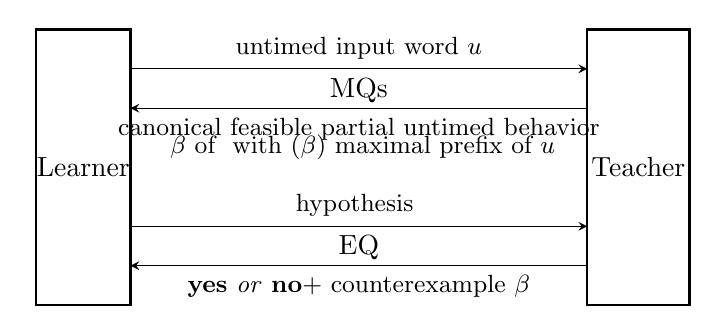
\begin{tikzpicture}[>=stealth]
            \draw [thick] (0,0) rectangle (1.2,3.5) node[midway] {Learner};
            \draw [thick] (7,0) rectangle (8.3,3.5) node[midway] {Teacher};
            \draw [->] (1.2,3) -- (7,3) node[midway,below] {MQs};
            \draw (1.2,3) -- (7,3) node[midway,above] {\small untimed input word $u$};
            \draw [<-] (1.2,2.5) -- (7,2.5) node[midway,below] {\small canonical feasible partial untimed behavior};
             \draw (4.15,2) node {\small $\beta$ of $\M$ with $\untimedinputword(\beta)$ maximal prefix of $u$};
            \draw [->] (1.2,1) -- (7,1) node[midway,below] {EQ};
            \draw (1.2,1) -- (7,1) node[midway,above] {\small hypothesis $\CH$};
            \draw [<-] (1.2,0.5) -- (7,0.5) node[midway,below] {\small {\bf yes} \emph{or} {\bf no}+ counterexample $\beta$};
        \end{tikzpicture}
\end{center}    
\caption{Untimed MAT framework}
\label{fig:untimed MAT}
\end{figure}

Our untimed learning setup, illustrated in Figure~\ref{fig:untimed MAT}, is similar to the timed setup:
again the teacher knows an MMT $\M$ and the learner initially only knows the set of inputs $I$ of $\M$.
Again, the learer may pose membership and equivalence queries.
But now a \emph{membership query} consists of an untimed input word $u$ over $I$.
The teacher replies with a maximal feasible partial untimed behavior $\beta$ of $M$ (in canonical form) such that
$\untimedinputword(\beta)$ is a prefix of $u$.
With an \emph{equivalence query}, the learner asks if a hypothesis $\CH$ with inputs $I$ is correct.
Upon receiving $\CH$, the teacher answers \emph{yes} if $\CH \approx_{\mathit{untimed}} \M$.
Otherwise it answers \emph{no} and supplies a counterexample, which now is a feasible untimed behavior $\beta$ (in canonical form) that
is a partial untimed behavior of $\M$ but not of $\CH$ (by Lemma~\ref{not untimed} such a counterexample exists).

\subsection{Zones and constraints}

In order to implement an untimed teacher using a timed teacher, we need a
basic machinery to determine whether an untimed behavior is feasible, i.e.,
whether it can be derived from a timed word. This can be done using
well-established techniques for manipulating difference-bound matrices
(DBMs) that are in standard use for analyzing timed
automata~\cite{Di89,BengtssonY03}.
In this section, we describe an adaptation of such techniques to
our setting.

Let $\beta$ be an untimed behavior in canonical form:
\begin{eqnarray*}
\beta & = & \emptyset \uttrans{i_1}{o_1}{\rho_1} X_1  \cdots X_{k-1} \uttrans{i_k}{o_k}{\rho_k} X_k.
\end{eqnarray*}
We would like to determine for which values $d_1, \ldots , d_{k+1}$
a corresponding timed behavior
\[
\tvals_0 \dtrans{d_1} \tvals'_0 \uttrans{i_1}{o_1}{\rho_1}
\quad \cdots \quad
\dtrans{d_k} \tvals'_k \uttrans{i_k}{o_k}{\rho_k} \tvals_k
\dtrans{d_{k+1}} \tvals'_{k+1}
%% \uttrans{\toevent{x_i}}{o_{n+1}}{\rho_n}
\]
is possible. We solve this problem by producing a constraint over the
values $d_1, \ldots , d_{k+1}$. In order to use DBM techniques, we first
change representation by letting
$t_j = d_1 + \cdots + d_j$ for $j = 1 , \ldots, k+1$. Intuitively, $t_j$ is
the time of occurrence of the $j$th transition in $\beta$.
We now associate with $\beta$ a conjunction of difference constraints over
$t_1, \ldots, t_{k+1}$, denoted $\Constraints{\beta}$, consisting of
%\todobj{We assume that delays are always non-zero. Check how this is said in the paper}
\begin{itemize}
%% \item
%% $0 < t_1 \leq d_{\max}$,
%% \item
%% for each index $j < k$:  $0 <  t_{j+1} - t_j \leq d_{\max}$,
\item
for each index $j$ with $1 \leq j \leq k$:  $0 <  t_{j+1} - t_j$,
\item
for each timeout event $i_j = \toevent{x_l}$: $t_j - t_l = \rho_l(x_l)$,
\item
for each clock $x_l$ that is started but does not timeout: $t_j -t_l < \rho_l(x_l)$,
where $j$ is the largest index such that $x_l \in X_j$,
%% \item
%% for each pair of distinct indices $j$ and $l$ with $i_j, i_l \in I$: $\Frac{t_j} \neq \Frac{t_l}$ 
%% (to express that the fractional parts of $t_j$ and $t_l$ are different).
\end{itemize}
By standard DBM techniques, we can check whether $\Constraints{\beta}$ is satisfiable by saturating it (i.e., closing it under implied constraints, which
will always be of form
$n < t_j - t_l < m$ or $t_j - t_l = m$ for integers $n,m$), and checking that
all such differences allow $t_{j+1} - t_j$ be positive for each $j$.
We infer that $\beta$ is feasible iff $\Constraints{\beta}$ is satisfiable.
Moreover, if $\beta$ is feasible, it is easy to see that there is a solution
such that $\Frac{t_j} \neq \Frac{t_l}$ for each pair of distinct indices $j$ and $l$ with $i_j, i_l \in I$.

From the saturated version of $\Constraints{\beta}$, we also derive a constraint,
denoted $\Zone{\beta}$,
which characterizes the possible timer valuations $\tvals_k$ in a timed
behavior of the above form.  The constraint $\Zone{\beta}$
contains for each pair of timers $x_i,x_j$ in $X_k$ the conjunct
\[
(m + \rho_j(x_j) - \rho_i(x_i)) < \tvals_k(x_j) -\tvals_k(x_i) < (n + \rho_j(x_j) - \rho_i(x_i))
\]
whenever the saturated version of $\Constraints{\beta}$ contains the conjunct
\(
m < t_j - t_i < n
\).
(This can be derived using
$\tvals_k(x_j) = \rho_j(x_j) - (t_k - t_j)$
and
$\tvals_k(x_i) = \rho_i(x_i) - (t_k - t_i)$).

We can derive the following lemmas.

\begin{lemma}
\label{lemma: feasibility concatenation}
Suppose $\beta, \beta'$ are untimed behaviors such that
$\Zone{\beta} = \Zone{\beta'}$. Let $\gamma$ be any untimed behavior.
Then $\beta \cdot \gamma$ is feasible iff $\beta' \cdot \gamma$ is feasible.
\end{lemma}

\begin{lemma}
\label{lemma finitely many zones}
$\{ \Zone{\beta} \mid \beta \mbox{ feasible untimed behavior of } \M \}$ is finite.
\end{lemma}
\begin{proof}
  An MMT only has a finite number of timers that can only be set to a finite number of integer values. Since in an MMT the values of timers can only decrease, their values are bounded, so that only finitely many integers may appear in the conjuncts of $\Zone{\beta}$. This the set of possible $\Zone{\beta}$ is finite.
\end{proof}

Let $\beta$ be a feasible untimed behavior and let $x \in X$ be a timer. Then we say that $x$ is \emph{expirable} after $\beta$
if there exists a valuation in $\Zone{\beta}$ in which $x$ is minimal.

\begin{lemma}
\label{expirable}
Suppose $\beta$ is a feasible untimed behavior with $\Last{\beta} = Y$ and $Y \uttrans{\toevent{x}}{o}{\rho} Y'$ is an untimed behavior.
Then $x$ is expirable after $\beta$ iff $\beta \uttrans{\toevent{x}}{o}{\rho} Y'$ is feasible.
\end{lemma}


%Note that for an untimed behavior $\beta$, the set $\zone{\beta}$ of valuations that can be reached with a timed behavior $\sigma$ with %$\untime(\sigma) = \beta$ can be symbolically represented using DBMs \cite{Di89}.
%We can do this since the transition relations $\xrightarrow{d}$ and $\xrightarrow{i_1/o_1, \rho_1}$ can be decomposed 
%into elementary operations on DBMs such as reset, conjunction, and delay successors \cite{BengtssonY03}.
%This allows us to compute whether an untimed behavior $\beta$ is feasible ($\zone{\beta}$ is empty), and
%whether a timer $x$ may expire after $\beta$ ($\zone{\beta}$ contains a valuation in which $x$ is minimal).

\subsection{Building an untimed teacher from a timed teacher}
We will now show how to construct an adapter that transforms a teacher for the timed setting into a teacher for the untimed setting.
The adapter maintains an integer variable $d_{\max}$ to store an estimate of the maximal timeout value that occurs in $\M$. Initially, the
adapter sets $d_{\max}$ to an arbitrary value, which may be increased based on the (transparent) timed words that it receives from
the timed teacher.

Suppose the untimed teacher receives a membership query, consisting of an untimed input word
$u = i_1 \cdots i_k$.
By induction on the length of $u$, 
we construct a response for $u$, that is, a feasible partial untimed behavior $\beta_k$ of $\M$ (in canonical form)
with $\untimedinputword(\beta_k)$ a maximal prefix of $u$.
If $k=0$, then response $\beta_0$ is the trivial partial untimed behavior $\emptyset$.
For the induction step, suppose that $k>0$.
Let $\beta_{k-1}$ be the response for $i_1 \cdots i_{k-1}$.
If $\beta_{k-1}$ contains less than $k-1$ inputs, then response $\beta_k$ is equal to $\beta_{k-1}$.
Now assume that $\beta_{k-1}$ contains $k-1$ inputs. We consider two cases:
\begin{enumerate}
\item
$i_k \in I$. Set $\beta := \beta_{k-1} ~ i_k ~ \omega ~ \emptyset$, where $\omega \in O$ is an arbitrary output that acts as placeholder.
Since $\beta_{k-1}$ is feasible (by induction hypothesis), it follows by Lemma~\ref{feasible plus input is feasible} that
$\beta$ is also feasible.
Thus the constraints in $\Constraints{\beta}$ are satisfiable and we may compute a solution $t_1 ,\ldots, t_k$.
Let $o_1 ,\ldots, o_{k-1}$ be the outputs occurring in $\beta_{k-1}$. Then
$w = t_1 ~ i_1 ~ o_1 ~ t_2 - t_1 ~ i_2 ~ o_2 ~ t_3- t_2 \cdots t_k - t_{k-1} ~ i_k ~ \omega$ is a transparent timed word.
Let $u' = \timedinputword(w)$ be the transparent timed input word associated to $w$.
We forward membership query $u'$ to the timed teacher.
Let $w'$ be the response from the timed teacher.
If $w'$ and $w$ are equal, except possibly for the last output symbol, which is $o_k$ in $w'$,
the response $\beta_k$ is equal to $\beta_{k-1} ~ i_k ~ o_k ~ \emptyset$.
Otherwise, $w'$ contains some timeout event that was not supposed to happen according to untimed input word $u$.
Since $u'$ is transparent, $w'$ is transparent as well. Thus we may extract from $w'$ which event $l$ started the timer, to which value
$d$ the timer was set, and the index $j$ of the timeout event.
We set $\beta_{k-1} := \Addtimer{l}{d}{j-1}{\beta_{k-1}}$ and perform step (1) again. 
Note that the number of iterations is linear in the size of $u$.
\item
$i_k = \toevent{x_l}$, for $l < k$.
If $\beta_{k-1}$ assigns value $e$ to timer $x_l$ then
we set $\beta := \Addtimer{l}{e}{k-1}{\beta_{k-1}} ~ \toevent{x_l} ~ \omega ~ \emptyset$ and check whether $\Constraints{\beta}$ is
satisfiable. If not then response $\beta_k$ is equal to $\beta_{k-1}$.
If $\beta_{k-1}$ does not assign a value to $x_l$ then define, for $1 \leq e \leq d_{\max}$,
$\beta^e = \Addtimer{l}{e}{k-1}{\beta_{k-1}} ~ \toevent{x_l} ~ \omega ~ \emptyset$.
Search for an $e$ for which $\Constraints{\beta^e}$ is satisfiable and set $\beta := \beta^e$.
If there is no such $e$ then response $\beta_k$ is equal to $\beta_{k-1}$.
Otherwise, we compute a solution $t_1 ,\ldots, t_k$ for $\Constraints{\beta}$.
Let $o_1 ,\ldots, o_{k-1}$ be the outputs occurring in $\beta_{k-1}$. Then
$w = t_1 ~ i_1 ~ o_1 ~ t_2 - t_1 ~ i_2 ~ o_2 ~ t_3- t_2 \cdots t_k - t_{k-1} ~ \toevent{x_l} ~ \omega$ is a transparent timed word.
Let $u' = \timedinputword(w)$ be the transparent timed input word associated to $w$.
We forward membership query $u'$ to the timed teacher.
Let $w'$ be the response from the timed teacher. Since $u'$ is transparent, $w'$ is transparent as well.
If $w'$ and $w$ are equal, except possibly for the last output symbol, which is $o_k$ in $w'$,
the response $\beta_k$ is equal to $\beta$ with the last output set to $o_k$.
It may also occur that, even though the last event of $w'$ is a timeout triggered by event $i_l$, the value $e'$ to which this timer is
set is different from $e$. In this case response $\beta_k$ is set to
$\beta_k = \Addtimer{l}{e'}{k-1}{\beta_{k-1}} ~ \toevent{x_l} ~ o_k ~ \emptyset$, where $o_k$ is the last output in $w'$.
Finally, it may occur that $w'$ contains some timeout event that was not supposed to happen according to untimed input word $u$.
In this case, we extract from $w'$ which event $l$ started the timer, to which value
$d$ the timer was set, and the index $j$ of the timeout event.
We set $\beta_{k-1} := \Addtimer{l}{d}{j-1}{\beta_{k-1}}$ and perform step (2) again. 
Again the number of iterations is linear in the size of $u$.
\end{enumerate}
\todofv{Add example!}
%\paragraph{Example}
%Consider a scenario where the timed teacher knows the MMT of Figure~\ref{fig:nondeterminism} (bottom).
%Suppose that $d_{\max} = 5$ and the untimed teacher receives a query for input word $i ~ i$. The adapter starts with defining
%\[
%\beta_0 = \emptyset
%\]
%Next it solves $\Constraints{\emptyset ~ i ~ \omega ~ \emptyset} = \{ 0 < t_1 \leq 5 \}$.
%Suppose it arrives at the solution $t_1 = 1$. Based on this, the timed input word $1 ~ i ~ 0$ is
%forwarded to the timed teacher. The timed teacher responds with $1 ~ i ~ o$ and the adapter defines
%\[
%\beta_1 = \emptyset ~ i ~ o ~ \emptyset
%\]
%The constraints in $\Constraints{\emptyset ~ i ~ o ~ \emptyset ~ i ~ \omega ~ \emptyset}$ are still trivial.
%Suppose adapter finds solution $t_1 = 1,~ t_2 = 4.1$ and forwards timed input word  $1 ~ i ~ 3.1 ~ i ~ 0$ to the timed teacher.
%Based on the response $1 ~ i ~ o ~ 2 ~ \mathit{to} ~ o$, the adapter realized that the first transition starts a timer
%and solves $\Constraints{\emptyset ~ i,x:=1 ~ o ~ \{ x \} ~ i ~ \omega ~ \emptyset}$.

Implementing equivalence queries is easy.
Suppose that the untimed teacher receives an equivalence query $\CH$.
Then we just forward this query to the timed teacher.
If the timed teacher answers \emph{yes} then $\CH \approx_{\mathit{timed}} \M$.
In this case, by Theorem~\ref{timedimpliesuntimed}, $\CH \approx_{\mathit{untimed}} \M$,
and thus the untimed teacher should also return the result \emph{yes}.
If the timed teacher answers \emph{no} and returns a counterexample $w$,
then $w$ is a transparent timed word of $\M$ but not of $\CH$.
In this case, by Theorem~\ref{untimedimpliestimed}, we may conclude that
$\CH \not\approx_{\mathit{untimed}} \M$, and thus the untimed teacher should also return a result \emph{no}.
Since $w$ is a transparent timed word of $\M$, it 
follows by Lemma~\ref{lemma unique causality map} that $w$ 
has a unique causality map $c$.
This allows us to transform $w$ into a feasible untimed behavior $\beta$ (in canonical form) that is a partial untimed
behavior of $\M$ but not of $\CH$: the causality map tells us exactly which timers are set and timeout. 
Thus the untimed teacher may return $\beta$ as counterexample.
If our estimate $d_{\max}$ of the maximal timeout value of $\M$ is too low, then it may occur that in $w$ the timeout value of some
timer is larger than $d_{\max}$. In this case, the value of $d_{\max}$ is updated to the newly observed maximal timeout value.
\todofv{Think through implications of updating $d_{\max}$.}






%% \subsection{A Myhill Nerode Theorem for MMTs}

\begin{definition}
Let $S$ be a set of feasible untimed behaviors in canonical form over $I$ and $O$. Then $S$ is
\emph{prefix closed} if $\beta \beta' \in S \Rightarrow \beta \in S$,
\emph{behavior deterministic} if
$\beta \xrightarrow{i/o_1, \rho_1} X_1 \in S \wedge \beta \xrightarrow{i/o_2, \rho_2} X_2 \in S \Rightarrow o_1 = o_2 \wedge \rho_1 = \rho_2 \wedge X_1 = X_2$,
\emph{input complete} if
$\beta \in S \wedge i \in I \Rightarrow \exists o, \rho, Y : \beta \xrightarrow{i/o, \rho} Y \in S$,
and
\emph{timeout complete} if
$\beta \in S \wedge x \mbox{ expirable after } \beta \Rightarrow
\exists o, \rho, Y: \beta \xrightarrow{\toevent{x}/o, \rho} Y \in S$.

Suppose $\beta$ and $\beta'$ are behaviors in $S$ with $\Last{\beta} = X$ and $\Last{\beta'} = X'$.
Then $\beta$ and $\beta'$ are \emph{equivalent}, written $\beta \equiv_S \beta'$, iff there exists a bijection
$f_0 : X \to X'$ such that for any untimed behavior $\gamma$:
(a) if $\beta \cdot \gamma \in S$ then there exists an isomorphism $f$ that extends $f_0$ such that $\beta' \cdot f(\gamma) \in S$, and conversely,
(b) if $\beta' \cdot \gamma \in S$ then there exists an isomorphism $f$ that extends $f_0^{-1}$ such that $\beta \cdot f(\gamma) \in S$.
We write $[\beta]$ to denote the equivalence class of $\beta$ with respect to $\equiv_S$.
\end{definition}

\begin{theorem}
\label{Myhill Nerode}
Let $S$ be a set of feasible untimed behaviors in canonical form over finite sets of inputs $I$ and outputs $O$.
Then there exists an MMT with feasible untimed behaviors $T$ such that $S = \can{T}$ iff 
$S$ is nonempty, all untimed behaviors in $S$
start with the empty set of timers, $S$ is prefix closed, 
there is a bound on the number of timers that can be active simultaneously 
($\exists n \in \nat ~ \forall \beta \in S : \mid \Last{\beta} \mid \leq n$),
$S$ is behavior deterministic, input complete, timeout complete,
and $\equiv_S$ has only finitely many equivalence classes (finite index).
\end{theorem}
\iflong
\begin{proof} (Needs work)

``$\Rightarrow$'' Let $\M$ be an MMT, let $T$ be its set of feasible untimed behaviors, and let $S = \can{T}$.
Then it is immediate from the definitions that $T$ is nonempty, all untimed behaviors in $S$
start with the empty set of timers, 
$S$ is prefix closed, 
there is a bound on the number of timers that can be active simultaneously,
$S$ is behavior deterministic, input complete, and timeout complete.
Suppose that $\beta, \beta' \in S$.
Then there exist (unique) $\beta_1, \beta'_1 \in T$ with
$\can{\beta_1}=\beta$ and $\can{\beta'_1}=\beta'$.
Suppose $\beta_1$ and $\beta'_1$ lead to the same state $q$ and moreover $\Post_{\beta_1} = \Post_{\beta'_1}$.
Since $\beta$ and $\beta_1$ are isomorphic, and $\beta'$ and $\beta'_1$ are isomorphic,
there exists a bijection $f_0 : X \to X'$ such that $f_0(\Post_{\beta}) = \Post_{\beta'}$.
Suppose that, for some untimed behavior $\gamma$, $\beta \gamma \in S$.
Then there exists an untimed behavior $\gamma_1$ such that $\beta_1 \gamma_1 \in T$ and $\can{\beta_1 \gamma_1} = \beta \gamma$.
By Lemma~\ref{lemma: feasibility concatenation},
$\beta'_1 \cdot \gamma_1 \in T$.
This implies $\beta' f(\gamma) \in S$ (elaborate this).
Since $\M$ only has finitely many states and by Lemma~\ref{lemma finitely many zones} the set
$\{ \Post_{\beta} \mid \beta \mbox{ is a feasible untimed behavior of } \M \}$ is finite, this means that
$\equiv_S$ has finite index.

``$\Leftarrow$'' Suppose $S$ is nonempty, etc.
Let $n$ be a bound on the number of timers that are active in a behavior in $S$ at any point.
We can construct a function that maps each untimed behavior $\beta \in S$
to an isomorphic behavior $\uncan{\beta}$ in such a way that only timers $\{ x_1 ,\ldots, x_n \}$ occur 
in all the behaviors in the range of $\mathit{uncan}$.
For instance, if a transition occurs in a state and this transition
starts a new timer, then $\mathit{uncan}$ may compute the smallest index $j$
such that $x_j$ is not unaffected by this transition, and then choose $x_j$ as the name of the new timer.
Let MMT $\M = (I, O \cup \{ \perp \}, Q, q_0, \vars, \delta, \lambda, \remap)$ be defined as follows:
\begin{itemize}
\item
$\perp$ is a special, fresh output event.
\item
$Q = \{ ( [\beta], \Post_{\uncan{\beta}}) \mid \beta \in S \}$.
\item
$q_0 = ([\emptyset], Z_0)$. (Note that $\emptyset \in S$ since $S$ is nonempty, prefix closed, and all untimed behaviors in $S$ start
with the empty set of timers; $Z_0$ is the unique zone for the empty set of variables.)
\item
$\varsof{([\beta], Z)} = \domof{Z}$.
\item
(rest needs doing). Let $\beta \in S$ and $i \in I$. Then, since $S$ is both input complete and behavior deterministic, there exist unique
$o$, $\rho$ and $Y$ such that $\beta' = \beta \xrightarrow{i/o, \rho} Y \in S$.
We define $\delta([\beta],i) = [\beta']$, $\lambda([\beta],i) = o$, and $\remap([\beta],i) = \rho$.
\item
Assume $\beta \in S$ and $x\in \Last{\beta}$ expirable after $\beta$. 
Then, since $S$ is both timeout complete and behavior deterministic, there exist unique
$o$, $\rho$ and $Y$ such that $\beta' = \beta \xrightarrow{\toevent{x}/o, \rho} Y \in S$.
We define $\delta([\beta],\toevent{x}) = [\beta']$, $\lambda([\beta],\toevent{x}) = o$, and $\remap([\beta],\toevent{x}) = \rho$.
\item
Assume $\beta \in S$ and $x \in \Last{\beta}$ not expirable after $\beta$.
We define $\delta([\beta],\toevent{x}) = [\beta]$, $\lambda([\beta],\toevent{x}) = \perp$, and $\remap([\beta],\toevent{x}) = \rho_0$, where $\domof{\rho_0} = \emptyset$.
\end{itemize}
It is routine to verify that $\M$ is a well-defined MMT whose set of feasible untimed behaviors equals $S$.
\end{proof}
\fi

\section{Another Try on ``Zones and constraints''}

In order to implement an untimed teacher using a timed teacher, we need a
basic machinery to determine whether an untimed behavior is feasible, i.e.,
whether it can be derived from a timed word. This can be done using
well-established techniques for manipulating difference-bound matrices
(DBMs) that are in standard use for analyzing timed
automata~\cite{Di89,BengtssonY03}.
In this section, we describe an adaptation of such techniques to
our setting.

Let $\beta$ be an untimed behavior in canonical form:
\begin{eqnarray*}
\beta & = & \emptyset \uttrans{i_1}{o_1}{\rho_1} X_1  \cdots X_{k-1} \uttrans{i_k}{o_k}{\rho_k} X_k.
\end{eqnarray*}
We would like to determine for which values $d_1, \ldots , d_{k+1}$
a corresponding timed behavior
\[
\tvals_0 \dtrans{d_1} \tvals'_0 \uttrans{i_1}{o_1}{\rho_1}
\quad \cdots \quad
\dtrans{d_k} \tvals'_k \uttrans{i_k}{o_k}{\rho_k} \tvals_k
\dtrans{d_{k+1}} \tvals'_{k+1}
%% \uttrans{\toevent{x_i}}{o_{n+1}}{\rho_n}
\]
is possible. We solve this problem by producing a constraint over the
values $d_1, \ldots , d_{k+1}$. In order to use DBM techniques, we first
change representation by letting
$t_j = d_1 + \cdots + d_j$ for $j = 1 , \ldots, k+1$. Intuitively, $t_j$ is
the time of occurrence of the $j$th transition in $\beta$.
We now associate with $\beta$ a conjunction of difference constraints, denoted
$\Constraints{\beta}$, consisting of
\todobj{We assume that delays are always non-zero. Check how this is said in
  the paper}
\begin{itemize}
%% \item
%% $0 < t_1 \leq d_{\max}$,
%% \item
%% for each index $j < k$:  $0 <  t_{j+1} - t_j \leq d_{\max}$,
\item
for each index $j$ with $1 \leq j \leq k$:  $0 <  t_{j+1} - t_j$,
\item
for each timeout event $i_j = \toevent{x_l}$: $t_j - t_l = \rho_l(x_l)$,
\item
for each clock $x_l$ that is started but does not timeout: $t_j -t_l < \rho_l(x_l)$,
where $j$ is the largest index such that $x_l \in X_j$,
%% \item
%% for each pair of distinct indices $j$ and $l$ with $i_j, i_l \in I$: $\Frac{t_j} \neq \Frac{t_l}$ 
%% (to express that the fractional parts of $t_j$ and $t_l$ are different).
\end{itemize}
Using standard DBM techniques, we can check whether $\Constraints{\beta}$ is satisfiable by saturating it (i.e., closing it under implied constraints, which
will always be of form
$n < t_j - t_l < m$ and $t_j - t_l = m$ for integers $n,m$), and checking that
all such differences allow $t_{j+1} - t_j$ be positive for each $j$.
We infer that $\beta$ is feasible iff the set of constraints $\Constraints{\beta}$ is satisfiable.
Moreover, if $\beta$ is feasible, it is easy to see that there is a solution
such that $\Frac{t_j} \neq \Frac{t_l}$ for each pair of distinct indices $j$ and $l$ with $i_j, i_l \in I$.

From the saturated version of $\Constraints{\beta}$, we also derive a constraint,
denoted $\Zone{\beta}$,
which characterizes the possible timer valuations $\tvals_k$ in a timed
behavior of the above form.  The constraint $\Zone{\beta}$
contains for each pair of timers $x_i,x_j$ in $X_k$ the conjunct
\[
(m + \rho_j(x_j) - \rho_i(x_i)) < \tvals_k(x_j) -\tvals_k(x_i) < (n + \rho_j(x_j) - \rho_i(x_i))
\]
whenever the saturated version of $\Constraints{\beta}$ contains the conjunct
\(
m < t_j - t_i < n
\).
(This can be derived using
$\tvals_k(x_j) = \rho_j(x_j) - (t_k - t_j)$
and
$\tvals_k(x_i) = \rho_i(x_i) - (t_k - t_i)$).

We can derive the following lemmas.

\begin{lemma}
\label{lemma: feasibility concatenation}
Suppose $\beta, \beta'$ are untimed behaviors such that
$\Zone{\beta} = \Zone{\beta'}$. Let $\gamma$ be any untimed behavior.
Then $\beta \cdot \gamma$ is feasible iff $\beta' \cdot \gamma$ is feasible.
\end{lemma}

\begin{lemma}
\label{lemma finitely many zones}
$\{ \Zone{\beta} \mid \beta \mbox{ feasible untimed behavior of } \M \}$ is finite.
\end{lemma}
\begin{proof}
  An MMT only has a finite number of timers that can only be set to a finite number of integer values. Since in an MMT the values of timers can only decrease, their values are bounded, so that only finitely many integers may appear in the conjuncts of $\Zone{\beta}$. This the set of possible $\Zone{\beta}$ is finite.
\end{proof}

Let $\beta$ be a feasible untimed behavior and let $x \in X$ be a timer. Then we say that $x$ is \emph{expirable} after $\beta$
if there exists a valuation in $\Zone{\beta}$ in which $x$ is minimal.

\begin{lemma}
\label{expirable}
Suppose $\beta$ is a feasible untimed behavior with $\Last{\beta} = Y$ and $Y \uttrans{\toevent{x}}{o}{\rho} Y'$ is an untimed behavior.
Then $x$ is expirable after $\beta$ iff $\beta \uttrans{\toevent{x}}{o}{\rho} Y'$ is feasible.
\end{lemma}


\todofv{Move next lemma to earlier section}

\begin{lemma}
\label{not timed}
Suppose $\M, \N$ are MMTs with $\M \not\approx_{\mathit{timed}} \N$.
Then there exists a transparent timed word $w$ of $\M$ that is not a timed word of $\N$.
\end{lemma}



\section{Approximating the Nerode Equivalence}
\label{sec:approx}

In this section, we present an approximation of the Nerode equivalence on
untimed behaviors
defined in Definition~\ref{def:nerode}. This
approximated equivalence can be inferred using a finite set of membership
queries, and therefore be used as a basis for a learning algorithm,
analogously to the use of an approximated Nerode equivalence in
$L^*$~\cite{Ang87}.
Intuitively, it seems natural to parameterize such an equivalence by
a finite set $V$ of untimed input words (hereafter often
called {\em input suffixes}), by letting
untimed behaviors $\beta$ and $\beta'$ be equivalent
iff there exists a bijection $f_0 : X \to X'$ between the timers that are'active after $\beta$ and $\beta'$, respectively, such that whenever
$\untimedinputword(\gamma) \in V$, then
$\beta\cdot\gamma \in S$ iff 
$\beta'\cdot f_0(\gamma') \in S$, where $\gamma'$ is obtained by
renaming timers that are assigned in $\gamma$ in an appropriate way.
%% such that for any untimed behavior
%% $\gamma$ with $\untimedinputword(\gamma)\in V$:
%% if $\beta \cdot \gamma \in S$ then there exists an isomorphism $f$ that extends $f_0$ such that $\beta' \cdot f(\gamma) \in S$, and vice versa.
%% (b) if $\beta' \cdot \gamma \in S$ then there exists an isomorphism $f$ that extends $f_0^{-1}$ such that $\beta \cdot f(\gamma) \in S$.
In order to make this approach work, we must let the sets $V$ of suffixes that
parameterize the equivalence be
closed under permutation of timers that are active after a prefix $\beta$.
To illustrate why, consider a simple MMT, which can perform the untimed runs
\(
q_0 \uttrans{i_1}{o_1}{x_1:= 5} q_2
\)
or
\(
q_0 \simpleuttrans{i_1}{o_1} q_0 \uttrans{i_2}{o_2}{x_1:= 5} q_2
\),
and that from $q_2$ it can perform
\(
q_2 \simpleuttrans{\toevent{x_1}}{o_3} q_3
\).
The canonical untimed behaviors corresponding to the first two
untimed runs are
\(
\emptyset \uttrans{i_1}{o_1}{x_1:= 5} \set{x_1}
\)
and
\(
\emptyset \uttrans{i_1}{o_1}{} \emptyset \uttrans{i_2}{o_2}{x_2:= 5} \set{x_2}
\).
In order to let these two behaviors be equivalent we must discover that
timer $x_1$ can expire after the first one, and that
timer $x_2$ can expire after the second one. Since these two timers
have the same rules, the set $V$ of suffixes must
include the effects of the timeout events of form $\toevent{x_i}$ for any
timer $x_i$ that is assigned in a prefix, otherwise we
may fail to overapproximate the Nerode equivalence of Definition~\ref{def:nerode}.

Let us introduce notation to make the subsequent development more convenient. 
Recall that an untimed behavior is \emph{canonical} when, for each $j$,
the timer that is updated in the $j$-th event (if any) is equal to $x_j$.
It is {\em lean} if it is canonical and
includes only timers that expire during the behavior. 
Since the sequence of timer sets in a lean behavior is
uniquely determined by the labels on its transition, we can
denote a lean behavior simply by the sequence
$\utlabel{i_1}{o_1}{\rho_1} \cdots \utlabel{i_n}{o_n}{\rho_n}$ of its labels.
For behaviors that are to be appended as suffixes, we need to distinguish
timers that are assigned in the suffix from timers that are assigned in a prefix.
Therefore, extend the set of timers by the set $Y = \set{y_1,y_2,\ldots}$ of
{\em suffix timers}, which is disjoint from $X$.
Let $\toeventsof{Y}$ be the set of timeout events of form
$\toevent{y_i}$ for $y_i \in Y$, and let
$\extextinputs$ be $I \cup \toevents \cup \toeventsof{Y}$.
Define a {\em lean suffix behavior} to be a sequence
$\utlabel{i_1}{o_1}{\rho_1} \cdots \utlabel{i_m}{o_m}{\rho_m}$ of input/output/assignment triples,
in which each $i_j$ is in $\extextinputs$, 
each $\rho_j$ may assign only to the timer $y_j$,
each timeout event occurs at most once,
and all assigned timers in $Y$ expire sometime after their assignment.

For integer $k \geq 0$, let $\suffmap{k}$ be the injective mapping on
$Y$ which maps each $y_j$ to $y_{j+k}$.  We apply mappings of form
$\suffmap{k}$ to lean suffix behaviors in the natural way.

Let $\beta$ be a lean behavior. We say that 
a lean suffix behavior $\gamma$ is a {\em $\beta$-suffix} if
there is a canonical behavior $\beta'$ with $\beta \sqsubseteq \beta'$ such that
$\beta'\cdot\suffmap{|\beta|}(\gamma)$ is a lean behavior. In this case we
use $\beta;\gamma$ to denote $\beta'\cdot\suffmap{|\beta|}(\gamma)$.

Let an {\em input suffix} be a sequence of elements in $\extextinputs$.
A set $V$ of input suffixes is {\em adequate} if it is closed under permutations
on $X$ and includes all input suffixes of length one.
For an adequate set $V$ of input suffixes, and a lean behavior $\beta$,
let $\apprsuffixbehs{S}{\beta}{V}$ be the set of $\beta$-suffixes $\gamma$
with $\untimedinputword(\gamma) \in V$.
Let $\apprgetmemorable{S}{\beta}{V}$ be the set of timers $x_i$ in
$x_1 , \ldots x_{|\beta|}$ whose corresponding timeout event
(of form $\toevent{x_i}$) occurs (as an input) in some untimed behavior in
$\apprsuffixbehs{S}{\beta}{V}$.
Let $\apprgetassignment{S}{\beta}{V}$ map each timer $x_i$ in
$\apprgetmemorable{S}{\beta}{V}$ to the unique positive integer to which it
is assigned in the $i$th transition of $\beta$.


%% \todobj{Maybe we should point out that two prefixes $\beta$ and $\beta'$
%%   can be equivalent even if they assign corresponding timers to different
%%   values. However, timers assigned in corresponding suffixes must
%%   be assigned the same values.}

%% Let us introduce the {\em generic timeout event} $\toevent{p}$, where $p$w can
%% be regarded as a formal parameter,
%% which can be instantiated to an arbitrary timout event.
%% Let $(I \cup \set{\toevent{p}})^*$ be the set of
%% {\em generic untimed input words}.
%% An {\em instance} of a generic untimed input word is an untimed input
%% word obtained by replacing each generic timeout event
%% $\toevent{p}$ by a concrete timeout event.
%% For a set $V$ of generic untimed input words, let $\instancesof{V}$ be the
%% set of instances of words in $V$. For a canonical untimed
%% behavior $\beta$, let $\apprsuffixbehs{S}{\beta}{V}$ be the set of untimed behaviors
%% $\gamma$ with $\untimedinputword(\gamma) \in \instancesof{V}$ such that
%% $\beta\cdot\gamma$ is a canonical untimed behavior in $S$. Let
%% $\apprgetmemorable{S}{\beta}{V}$ be the set of timers $x_i$ in
%% $x_1 , \ldots x_{|\beta|}$ whose corresponding timeout event
%% (of form $\toevent{x_i}$) occurs (as an input) in some untimed behavior in
%% $\apprsuffixbehs{S}{\beta}{V}$.
%% Let $\apprgetassignment{S}{\beta}{V}$ map each timer $x_i$ in
%% $\apprgetmemorable{S}{\beta}{V}$ to the unique positive integer to which it
%% is assigned in the $i$th transition of that behavior.


%% Let $\suffbij{\beta}{\beta'}$ be the partial injective mapping
%% on timers that maps each
%% timer $x_i$ with $i > |\beta|$ to $x_{i + |\beta'| - |\beta|}$.
%% Intuitively, $\suffbij{\beta}{\beta'}$ maps a timer that is assigned 
%% in a transition of $\gamma$, where $\gamma$ is a suffix of the canonical
%% untimed behavior $\beta \cdot \gamma$, to the corresponding timer of
%% the canonical untimed behavior $\beta'\cdot\gamma$.
%% For two partial mappings $f$, $g$ on $X$, we let $f \sqcup g$ be their
%% union. \todobj{Does this need to be further clarified?}

%% \todobj{An illustrating example would help the reader here}

\todobj{We really need a few examples here}

We can now defined the approximated Nerode equivalence, which is parameterized
on an adequate set of lean input suffixes.

\begin{definition}
  \label{def:approx-nerode}
Let $S$ be a timer language \todobj{Define this},
let $\beta$ and $\beta'$ be canonical untimed behaviors in $S$,
and let  $V$ be an adequate set of lean input suffixes.
Let $f : \apprgetmemorable{S}{\beta}{V} \to \apprgetmemorable{S}{\beta'}{V}$
be a bijection
from $\apprgetmemorable{S}{\beta}{V}$ to $\apprgetmemorable{S}{\beta'}{V}$.
Then $\beta$ and $\beta'$ are \emph{equivalent wrp $V$} under $f$, written
$\beta \equiv_{S,V}^f \beta'$ iff
\[
\gamma \in \apprsuffixbehs{S}{\beta}{V}
\qquad \mbox{iff} \qquad
f(\gamma) \in \apprsuffixbehs{S}{\beta'}{V}
\]
\end{definition}
Intuitively, $\beta \equiv_{S,V}^f \beta'$ means that $\beta$ and $\beta'$
allow the same suffixes with inputs in $V$, after renaming
timers assigned in $\beta$ by $f$.
We write $\beta \equiv_{S,V} \beta'$ to denote that
$\beta \equiv_{S,V}^f \beta'$ for some
$f : \apprgetmemorable{S}{\beta}{V} \to \apprgetmemorable{S}{\beta'}{V}$.


\todobj{What theorems should we prove about this approximating equivalence?
  We should make the definition of Nerode use the same notation, whenever
  reasonable, to make this easier}

\section{Algorithm for Learning of MMTs}
\label{sec:learning}

In this section, we present an algorithm for learning MMTs in then untimed
MAT of~\ref{sec:untimed-mat}, using the approximated Nerode equivalence
presented in Section~\ref{sec:approx}.
The learning algorithm follows the standard pattern for active automata learning
algorithms, such as $L^*$~\cite{Ang87}. It maintains
a set $U$ of {\em short prefixes}, and
  an overapproximation of the Nerode equivalence,
  parameterized by a set $V$ of input suffixes.
Each short prefix in $U$ is a feasible canonical untimed
behavior, which represents a state in the MMT to be constructed.
The learning algorithm iterates two phases: hypothesis construction and
hypothesis validation.
During hypothesis construction,
the approximation of the Nerode equivalence triggers the expansion of
$U$ and $V$ until two convergence conditions are satisfied that allow
a hypothesis automaton to be formed.
During hypothesis validation, the hypothesis automaton is submitted in an
equivalence query, and returned counterexamples are used to refine
the Nerode equivalence by expanding $V$.

\todobj{Say somewhere that we assume a fixed (un)timed language $S$.}

Let us introduce the two conditions for convergence of the construction phase.
For a feasible untimed word $\beta$, let $\feasibleinputs{\beta}{S}$ be the
set of $i \in \extinputs$ such that there is a $\beta$-suffix of form
$\utlabel{i}{o}{\rho}$ for some $o$ and $\rho$.
For $i \in \feasibleinputs{\beta}{S}$, let $\lambda(\beta,i)$ be the unique
output $o$ such that $\utlabel{i}{o}{\rho}$ is a $\beta$-suffix for some $\rho$.
%% A set $V$ of generic untimed input words is {\em adequate} if it includes
%% $I \cup \set{\toevent{p}}$.
Let $U$ be a prefix-closed set of feasible lean behaviors.
and let $V$ be an adequate set of input suffixes.
\begin{itemize}
\item
$U$ is {\em closed} wrt.\ $V$ if 
  for each $\beta \in U$ and
  $i \in \feasibleinputs{\beta}{S}$
%%   , which is either in $I$ or of form $\toevent{x_i}$ where $x_i$ is expirable after $\beta$ if
  there is a $\beta' \in U$ such that
  $\beta;i/\lambda(\beta,i) \equiv_{S,V} \beta'$.
\item
$U$ is {\em timer-consistent} wrt.\ $V$ if 
  for each $\beta \in U$ and
  $i \in \feasibleinputs{\beta}{S}$
  %% $i$, which is either in $I$ or
  %% of form $\toevent{x_i}$ for $x_i$ expirable after $\beta$,
  we have
  $\apprgetmemorable{S}{\beta;\lambda(\beta,i)}{V} \subseteq
  (\apprgetmemorable{S}{\beta}{V} \cup \set{x_{(|\beta|+1)}})$.
\end{itemize}
Closedness ensures that each transition in the MMT to be constructed has a target location. 
Timer-consistency states that each timer which is needed after such
a transition (i.e., a timer set during $\beta;7O\lambda(\beta,i)$)
is either a timer active after $\beta$ or is started by the last transition, thus
getting the name $x_{(|\beta|+1)}$.
Closedness and timer-consistency allow the construction of a hypothesis MMT.

\todobj{Note that lean behaviors of form $\beta;i/\lambda(\beta,i),\rho$
  always have an empty $\rho$, hence we can omit $\rho$}

\begin{definition}[Hypothesis automaton]
\label{def:hypo}
  Let $U$ be a non-empty prefix-closed set of untimed behaviors,
  and $V$ an adequate set of input suffixes such that
  $U$ is closed and timer consistent wrt.\ $V$. Then the
{\em hypothesis automaton} $\hypoof UV$ is the MMT
$\hypoof UV = (I, O, Q, q_0, \vars, \delta, \lambda, \remap)$, where
\begin{itemize}
\item $Q = U$ and $q_0 = \emptyword$,
\item $\vars$ maps each location $\beta\in U$ to $\apprgetmemorable{S}{\beta}{V}$,
\item $\lambda$ maps each $\beta \in U$ and $i \in \feasibleinputs{\beta}{S}$ to
  the unique $o$ such that $\extend{\beta}{i}{o} \in S$. 
  %% $i$, either in $I$ or of form $\toevent{x_i}$, to the output observed in
  %% reponse to $i$ after $\beta$.
\item $\delta$ maps each $\beta \in U$ and
  $i \in \feasibleinputs{\beta}{S}$ to
  to the unique $\beta' \in U$ such that there is an $f$ with
  $\extend{\beta}{i}{\lambda(\beta,i)} \equiv_{S,V}^f \beta'$.
\item $\remap$
 maps each $\beta \in U$ and $i \in \feasibleinputs{\beta}{S}$ to
  the function
  $\remap(\beta,i):\apprgetmemorable{S}{\beta'}{V} \mapsto (\apprgetmemorable{S}{\beta}{V} \cup \natplus)$ defined as $\rho \circ f^{-1}$, where $\rho$ maps 
  timer $x_{(|\beta|+1)}$ to
$\apprgetassignment{S}{(\extend{\beta}{i}{\lambda(\beta,i)})}{V}(x_{(|\beta|+1)})$.
\end{itemize}
\end{definition}


Our learning algorithm iterates two phases: hypothesis construction and
hypothesis validation.
During hypothesis construction, 
the approximation of the Nerode equivalence triggers the expansion of
$U$ and $V$ until $U$ is closed and timer-consistent wrpt.\ $V$,
so that a hypothesis MMT can be formed.
During hypothesis validation, returned counterexamples are used to refine
the approximated Nerode equivalence by expanding $V$.

During {\bf hypothesis construction}, membership queries are performed:
\begin{itemize}
\item for all untimed input words of form $\untimedinputword(\beta) \cdot i$
   for $\beta \in U$ and $i \in \extinputs$: this allows to determine
   $\feasibleinputs{\beta}{S}$ and $\lambda(\beta,i)$
   for $\beta \in U$ and $i \in \feasibleinputs{\beta}{S}$.
\item
  for all untimed input words of form $\untimedinputword(\beta) \cdot v$ and
  $\untimedinputword(\beta) \cdot i \cdot v$, where
  $\beta \in U$, $v \in \instancesof{V}$, and
  $i \in \feasibleinputs{\beta}{S}$.
    This allows to compute the approximated Nerode equivalence $\equiv_{S,V}$ on
    the set of untimed words of form $\beta$ and
    $\extend{\beta}{i}{\lambda(\beta,i)}$ with
    $\beta \in U$ and $i \in \feasibleinputs{\beta}{S}$.
    Whenever the set $U$ is not closed wrt.\ $V$, then it is extended:
if there is some $\beta \in U$ and $i$ in $\feasibleinputs{\beta}{S}$
for which there is no $o$ and $\beta' \in U$ such that
$\extend{\beta}{i}{\lambda(\beta,i)} \equiv_{S,V} \beta'$, 
then $\extend{\beta}{i}{\lambda(\beta,i)}$ is added to $U$,
triggering new membership queries.
Whenever the set $U$ is not timer-consistent wrt.\ $V$, then $V$ is extended:
for timer $x_j$ in
$\apprgetmemorable{S}{\extend{\beta}{i}{\lambda(\beta,i)}}{V} \setminus (\apprgetmemorable{S}{\beta}{V} \cup \set{x_{(|\beta|+1)}})$, find an 
untimed behavior of form $\extend{\gamma}{\toevent{x_i}}{o'}$ in
$\apprsuffixbehs{S}{\extend{\beta}{i}{\lambda(\beta,i)}}{V}$.
Then add $i\cdot\untimedinputword(\gamma)\cdot\toevent{p}$ to $V$.
\end{itemize}

When $U$ is closed and timer-consistent wrt.\ $V$, then
a hypothesis MMT $\hypoof UV$ is constructed and
validated by submitting it in an equivalence query.
If the query returns ``yes'', then
the learning is completed, and $\hypoof UV$ accepts $S$.
If the query returns a counterexample word $\alpha$, this is used to extend
$V$ as follows. We assume w.l.o.g.\ that no proper prefix of $\alpha$ is
a counterexample. 
By the fact that $\alpha$ is a counterexample, there is a suffix
$i/o,\rho \cdot \gamma$ of $\alpha$
such that $\beta\cdot i/o,\rho \equiv_{S,V} \beta'$ but
$\beta \cdot i/o,\rho \cdot \gamma \in S \notiff \beta' \cdot \gamma \in S$
for some $\beta,\beta' \in U$.
(To se this, let $\alpha = i_1/o_1,\rho_1 \cdots i_n/o_n,\rho_n$, and
define the sequence $\beta_0, \beta_1, \ldots ,\beta_{n}$ of short prefixes
in $U$ by $\beta_0 = \emptyword$ and
$\beta_{j-1}i_j/o_j,\rho_j \equiv_{S,V} \beta_{i}$ for
$j = 1, \ldots n$, i.e., $\beta_0 \ldots \beta_n$ is the sequence of states
visited when $\hypoof UV$ processes $\alpha$.
Let $\gamma_j$ be the suffix $i_{j+1}/o_{j+1}\rho_{j+1} \cdots i_n/o_n,\rho_n$
of $\alpha$ of length $n-j$. 
By the fact that $\alpha$ is a counterexample, we have
$\beta_0\cdot\gamma_0 \in S \notiff  \beta_{n} \in S$, which implies that
$\beta_{j-1}\cdot\gamma_{j-1} \in S \notiff \beta_j\cdot\gamma_j \in S$
for some $j$;
we can then take $\beta_{j-1}$ as $\beta$ and $\beta_j$ as $\beta'$.)
This means that $\gamma$ is a new separating suffix, and that $V$ should be
extended with the $v$ such that
$\untimedinputword(\gamma) \in \instancesof{\set{v}}$
should be added to
$V$. After adding $v$ to $V$, $U$ is no longer closed
wrt.\ $V$, so the algorithm can resume a next round of
hypothesis construction, which will eventually generate a new hypothesis,
etc.

\todobj{Should we insert a pseudocode description of the algorithm?}

The algorithm enjoys the following properties, which are similar to those
enjoyed by active automata learning algorithms for regular languages,
e.g.,~\cite{Ang87}.

\begin{theorem}
  \label{thm:alg:termination}
Given an MMT $\M$ whose normal form has $n$ states, 
algorithm XXX terminates and produces an equivalence MMT in normal form
using at most $n$ equivalence queries, and
$Y$ untimer membership queries.
\end{theorem}
   
\begin{proof}
Starting from some initial approximations (e.g., the singleton
set consisting of the empty word), the sets $U$ and $V$ are
successively extended, until $U$ contains one element of each equivalence
class of $\equiv_{S}$, and $\equiv_{S,V}$ coincides with
$\equiv_{S}$. 
At termination the hypothesis is correct, by definition of equivalence query.
During the construction, $U$ will never contain two elements that are
equivalent wrp. $\M$.
Since each round of hypothesis construction and validation adds at least one
word to $U$, there can be at most $n$ equivalence queries.
\end{proof}

\todobj{This is to be fixed}
Since each equivalence query adds only one
word to $V$, this means that $|V| \leq n$ when the algorithm finishes,
implying that in total, at most $n^2|I|$ membership queries
will be performed during hypothesis construction.
During hypothesis
validation, at most $2\log(m)$ membership queries need be performed
(in addition to the equivalence query), where
$m$ is the length of the largest counterexample word returned.



\section{Algorithm for Learning of MMTs}
\label{sec:learning}

\todobj{The notation for concatenation between prefix and suffix may need
  checking in this section}

In this section, we present an algorithm for learning MMTs in then untimed
MAT of~\ref{sec:untimed-mat}, using the approximated Nerode equivalence
presented in Section~\ref{sec:approx}.
The learning algorithm follows the standard pattern for active automata learning
algorithms, such as $L^*$~\cite{Ang87}. It maintains
a set $U$ of lean behaviors, called {\em short prefixes}, which
represent states in the MMT to be constructed,
and an overapproximation of the Nerode equivalence,
parameterized by a set $V$ of input suffixes.
%% Each short prefix in $U$ is a feasible canonical untimed
%% behavior, which represents a state in the MMT to be constructed.
The learning algorithm iterates two phases: hypothesis construction and
hypothesis validation.
During hypothesis construction,
the approximation of the Nerode equivalence triggers the expansion of
$U$ and $V$ until two convergence conditions are satisfied that allow
a hypothesis automaton to be formed.
During hypothesis validation, the hypothesis automaton is submitted in an
equivalence query, and returned counterexamples are used to refine
the Nerode equivalence by expanding $V$.

\todobj{Say somewhere that we assume a fixed (un)timed language $S$.
  Make sure we make clear that it is the set of {\bf feasible} lean
behaviors of the SUL}

Let us introduce the two conditions for convergence of the construction phase.
For a feasible lean behavior $\beta$, let $\feasibleinputs{\beta}{S}$ be the
set of $i \in \extinputs$ such that
$\beta ; \simpleutlabel{i}{o} \in S$ for some $o$ (recall that the
last assignment of a lean behavior is always empty).
For $i \in \feasibleinputs{\beta}{S}$, let $\lambda(\beta,i)$ be the unique
output $o$ such that $\beta ; \simpleutlabel{i}{o} \in S$.
%% A set $V$ of generic untimed input words is {\em adequate} if it includes
%% $I \cup \set{\toevent{p}}$.
Let $U$ be a prefix-closed set of lean behaviors.
and let $V$ be an adequate set of input suffixes.
\begin{itemize}
\item
$U$ is {\em closed} wrt.\ $V$ if 
  for each $\beta \in U$ and
  $i \in \feasibleinputs{\beta}{S}$
%%   , which is either in $I$ or of form $\toevent{x_i}$ where $x_i$ is expirable after $\beta$ if
  there is a $\beta' \in U$ such that
  $\beta;\simpleutlabel{i}{\lambda(\beta,i)} \equiv_{S,V} \beta'$.
\item
$U$ is {\em timer-consistent} wrt.\ $V$ if 
  for each $\beta \in U$ and
  $i \in \feasibleinputs{\beta}{S}$
  %% $i$, which is either in $I$ or
  %% of form $\toevent{x_i}$ for $x_i$ expirable after $\beta$,
  we have
  $\apprgetmemorable{S}{\beta;\simpleutlabel{i}{\lambda(\beta,i)}}{V} \subseteq
  (\apprgetmemorable{S}{\beta}{V} \cup \set{x_{(|\beta|+1)}})$.
\end{itemize}
Closedness ensures that each transition in the MMT to be constructed has a target state. 
Timer-consistency states that each timer which is needed after such
a transition (i.e., a timer set during $\beta;\simpleutlabel{i}{\lambda(\beta,i)}$)
is either a timer active after $\beta$ or is started by the last transition, thus
getting the name $x_{(|\beta|+1)}$.
Closedness and timer-consistency allow the construction of a hypothesis MMT.

\begin{definition}[Hypothesis automaton]
\label{def:hypo}
  Let $U$ be a non-empty prefix-closed set of lean behaviors,
  and $V$ an adequate set of input suffixes such that
  $U$ is closed and timer consistent wrt.\ $V$. Then the
{\em hypothesis automaton} $\hypoof UV$ is the MMT
$\hypoof UV = (I, O, Q, q_0, \vars, \delta, \lambda, \remap)$, where
\begin{itemize}
\item $Q = U$ and $q_0 = \emptyword$,
\item $\vars$ maps each location $\beta\in U$ to $\apprgetmemorable{S}{\beta}{V}$,
\item Let $\beta \in U$ and $i \in \feasibleinputs{\beta}{S}$. Then
  \begin{itemize}
    \item $\lambda(\beta,i)$ is
     the unique $o$ such that $\extend{\beta}{i}{o} \in S$. 
    \item $\delta(\beta,i)$ is is
        the unique $\beta' \in U$ such that there is an $f$ with
  $\extend{\beta}{i}{\lambda(\beta,i)} \equiv_{S,V}^f \beta'$.
  \item $\remap(\beta,i):\apprgetmemorable{S}{\beta'}{V} \mapsto (\apprgetmemorable{S}{\beta}{V} \cup \natplus)$ is defined as $\rho \circ f^{-1}$, where $\rho$ maps timer $x_{(|\beta|+1)}$ to
$\apprgetassignment{S}{(\extend{\beta}{i}{\lambda(\beta,i)})}{V}(x_{(|\beta|+1)})$.
  \end{itemize}
\item When $\beta \in U$ and $i$ is of form $\toevent{x_j}$ in
  $\apprgetmemorable{S}{\beta}{V} \setminus \feasibleinputs{\beta}{S}$, we let
  $\lambda(\beta,i) = \bot$, 
  $\delta(\beta,i) = \beta$, and let
  $\remap(\beta,i)$ be the identity mapping on $\apprgetmemorable{S}{\beta}{V}$.
\end{itemize}
\end{definition}
The last case in the construction constructs a transition that is not feasible,
but which must anyway be present since its input is a timeout event for
 a timer which can expire after performing additional transitions from $\beta$.

 During {\bf hypothesis construction}, membership queries are performed order
 to construct the sets of form $\apprsuffixbehs{S}{\beta}{V}$ and
 $\apprsuffixbehs{S}{\extend{\beta}{i}{\lambda(\beta,i)}}{V}$ for $\beta \in U$.
 Moreoever, the sets $U$ and $V$ are expanded if needed to construct
 a hypothesis automaton.

 More precisely,
membership queries are first performed
  for all untimed input words of form $\untimedinputword(\beta) \cdot i$
   for $\beta \in U$ and $i \in \extinputs$: this allows to determine
   $\feasibleinputs{\beta}{S}$ and $\lambda(\beta,i)$
   for $\beta \in U$ and $i \in \feasibleinputs{\beta}{S}$.
   Thereafter, membership queries are performed
  for all untimed input words of form $\untimedinputword(\beta) \cdot v$ and
  $\untimedinputword(\beta) \cdot i \cdot v$, where
  $\beta \in U$, $v \in V$, and
  $i \in \feasibleinputs{\beta}{S}$. Note that one need only consider
  $v$ in which inputs from $\toevents$ concern timers in
  $\set{x_1, \ldots, x_{|\beta|}}$ (or in  $\set{x_1, \ldots, x_{(|\beta|+1)}}$).
  This allows to construct the sets of form $\apprsuffixbehs{S}{\beta}{V}$ and
  $\apprsuffixbehs{S}{(\extend{\beta}{i}{\lambda(\beta,i)})}{V}$
  for $\beta \in U$.
  It then allows to compute the approximated Nerode equivalence $\equiv_{S,V}$ on
  the set of lean behaviors of form $\beta$ and
  $\extend{\beta}{i}{\lambda(\beta,i)}$ with
  $\beta \in U$ and $i \in \feasibleinputs{\beta}{S}$.
  We then check whether $U$ and $V$ meet the convergence criteria.
  \begin{itemize}
    \item
  Whenever the set $U$ is not closed wrt.\ $V$, then it is extended:
if there is some $\beta \in U$ and $i$ in $\feasibleinputs{\beta}{S}$
for which there is no $\beta' \in U$ such that
$\extend{\beta}{i}{\lambda(\beta,i)} \equiv_{S,V} \beta'$, 
then $\extend{\beta}{i}{\lambda(\beta,i)}$ is added to $U$,
triggering new membership queries.
\item
  Whenever the set $U$ is not timer-consistent wrt.\ $V$, then $V$ is extended:
for timer $x_j$ in
$\apprgetmemorable{S}{\extend{\beta}{i}{\lambda(\beta,i)}}{V} \setminus (\apprgetmemorable{S}{\beta}{V} \cup \set{x_{(|\beta|+1)}})$, find a lean
suffix behavior of form $\extend{\gamma}{\toevent{x_j}}{o'}$ in
$\apprsuffixbehs{S}{(\extend{\beta}{i}{\lambda(\beta,i)})}{V}$, i.e.,
a suffix such that $x_j$ expires in the last transition. This expiration is
obviously missing from $\apprsuffixbehs{S}{\beta}{V}$. But, by
adding $i\cdot\untimedinputword(\gamma)\cdot\toevent{x_j}$ to $V$, the
timer will also appear in $\apprgetmemorable{S}{\beta}{V}$.
This extension of $V$ will trigger new membership queries.
\end{itemize}
When $U$ is closed and timer-consistent wrt.\ $V$, then
a hypothesis MMT $\hypoof UV$ is constructed and
validated by submitting it in an equivalence query.
If the query returns ``yes'', then
the learning is completed, and $\hypoof UV$ accepts $S$.
If the query returns a counterexample in the form of a lean behavior
$\alpha$, this is used to extend $V$ as follows.
We assume w.l.o.g.\ that no proper prefix of $\alpha$ is a counterexample. 
By the fact that $\alpha$ is a counterexample, we can write $\alpha$ as
$(\alpha';\simpleutlabel{i}{o}); \gamma$, where $\gamma$ is a lean suffix
behavior such that
$\beta\cdot \simpleutlabel{i}{o} \equiv_{S,V}^f \beta'$ but
$(\beta ; \simpleutlabel{i}{o}) ; \gamma) \in S \notiff \beta' ; f(\gamma) \in S$ for some $\beta,\beta' \in U$ such that 
$\beta;\simpleutlabel{i}{o} \equiv_{S,V}^f \beta'$ is used to construct
the transition triggered by $i$ from $\beta$ in $\hypoof UV$.
\todobj{The rest still to be polished}
(To se this, let $\alpha = \utlabel{i_1}{o_1}{\rho_1} \cdots \utlabel{i_n}{o_n}{\rho_n}$, and
define the sequence $\beta_0, \beta_1, \ldots ,\beta_{n}$ of short prefixes
in $U$ and mappings $\pi_1, \ldots , \pi_n$ by $\beta_0 = \emptyword$ and
$\beta_{j-1}\utlabel{i_j}{o_j}{\rho_j} \equiv_{S,V} \beta_{i}$ for
$j = 1, \ldots n$, i.e., $\beta_0 \ldots \beta_n$ is the sequence of states
visited when $\hypoof UV$ processes $\alpha$. Let $\gamma_j$ be the suffix
$\utlabel{i_{j+1}}{o_{j+1}}{\rho_{j+1}} \cdots \utlabel{i_n}{o_n}{\rho_n}$
of $\alpha$ of length $n-j$. 
By the fact that $\alpha$ is a counterexample, we have
$\beta_0\cdot\gamma_0 \in S \notiff  \beta_{n} \in S$, which implies that
$\beta_{j-1}\cdot\gamma_{j-1} \in S \notiff \beta_j\cdot\gamma_j \in S$
for some $j$;
we can then take $\beta_{j-1}$ as $\beta$ and $\beta_j$ as $\beta'$.)
This means that $\gamma$ is a new separating suffix, and that $V$ should be
extended with the $v$ such that
$\untimedinputword(\gamma) \in \instancesof{\set{v}}$
should be added to
$V$. After adding $v$ to $V$, $U$ is no longer closed
wrt.\ $V$, so the algorithm can resume a next round of
hypothesis construction, which will eventually generate a new hypothesis,
etc.

\todobj{Should we insert a pseudocode description of the algorithm?}

The algorithm enjoys the following properties, which are similar to those
enjoyed by active automata learning algorithms for regular languages,
e.g.,~\cite{Ang87}.

\begin{theorem}
  \label{thm:alg:termination}
Given an MMT $\M$ whose normal form has $n$ states, 
algorithm XXX terminates and produces an equivalence MMT in normal form
using at most $n$ equivalence queries, and
$Y$ untimer membership queries.
\end{theorem}
   
\begin{proof}
Starting from some initial approximations (e.g., the singleton
set consisting of the empty word), the sets $U$ and $V$ are
successively extended, until $U$ contains one element of each equivalence
class of $\equiv_{S}$, and $\equiv_{S,V}$ coincides with
$\equiv_{S}$. 
At termination the hypothesis is correct, by definition of equivalence query.
During the construction, $U$ will never contain two elements that are
equivalent wrp. $\M$.
Since each round of hypothesis construction and validation adds at least one
word to $U$, there can be at most $n$ equivalence queries.
\end{proof}

\todobj{This is to be fixed}
Since each equivalence query adds only one
word to $V$, this means that $|V| \leq n$ when the algorithm finishes,
implying that in total, at most $n^2|I|$ membership queries
will be performed during hypothesis construction.
During hypothesis
validation, at most $2\log(m)$ membership queries need be performed
(in addition to the equivalence query), where
$m$ is the length of the largest counterexample word returned.


%%\newcommand{\natplus}{\nat^{>0}}
%\newcommand{\realsplus}{\bbbr^{\geq 0}}
%\newcommand{\stoptimer}{\mathit{kill}}
%\newcommand{\tosymbol}{\mathit{to}}
%\newcommand{\toevent}[1]{\mathit{to}[#1]}
%\newcommand{\toevents}{\mbox{\sl TO}}
%\newcommand{\extinputs}{\hat{I}}
\newcommand{\acttimers}{\mathit{active}}
%\newcommand{\expirable}{\mathit{expirable}}
%\newcommand{\tvals}{\kappa}
%\newcommand{\delay}[2]{t_{[#1:#2]}}
%\newcommand{\timerof}[2]{x_{#1}^{#2}}
\newcommand{\constrof}[1]{\phi_{#1}}
\newcommand{\post}{\mathit{post}}

%\newcommand{\conc}{\cdot}
%\newcommand{\tuple}[1]{\langle #1\rangle}
%\newcommand{\set}[1]{\lbrace #1\rbrace}
%\newcommand{\vect}[2]{{#1}_1 , \ldots , {#1}_{#2}}
%\newcommand{\setcomp}[2]{\set{#1 ~:~ #2}}
%\newcommand{\domof}[1]{\dom(#1)}
%\newcommand{\ranof}[1]{\ran(#1)}
%\newcommand{\vars}{\mathcal{X}}
%\newcommand{\varsof}[1]{\vars(#1)}
\newcommand{\ctimers}{X}
%\newcommand{\remap}{\pi}
%\newcommand{\remapinst}{\rho}
\newcommand{\normalize}{\gamma}
\newcommand{\normalizeof}[2]{\normalize_{#2}^{#1}}
\newcommand{\timerbij}{\gamma}
\newcommand{\timerequiv}{\pi}
\newcommand{\extendedby}{\lhd}
\newcommand{\uttrace}{\textsf{tr}}
\newcommand{\uttraceof}[1]{\uttrace(#1)}
\newcommand{\uttracesof}[1]{\textsf{Tr}(#1)}
\newcommand{\strace}{\textsf{tr}_s}
\newcommand{\ssuffix}{v_s}
\newcommand{\suftraces}{\textsf{Tr}_s}
\newcommand{\pinpof}[1]{\textit{inp}_p(#1)}
\newcommand{\sinpof}[1]{\textit{inp}_s(#1)}
\newcommand{\symbinpof}[1]{\textit{symbinp}(#1)}
\newcommand{\word}{w}
\newcommand{\smap}{{\cal O}}
\newcommand{\smappre}{{\cal O_p}}
\newcommand{\smapsuf}{{\cal O_s}}
\newcommand{\obspre}{{\cal O_U}}

\section{General Treatment for Arbitrary Number of Timers}

It is now time to consider the general case of
Mealy machines with an arbitrary number of timers (MMnT). 
These just generalize MM1Ts in that they have a set of timers that
can be manipulated in the same way as the timer of a MM1T.
We assume an unbounded set $X$ of {\em timers};
we use $x$, $x_1$, $x_2$, etc.\ to range over timers.
Let $\toevents$ be the set of {\em timeout events} of form
$\toevent{x}$ for $x \in X$.
For a set $I$, let $\extinputs$ be $I \cup \toevents$.

\begin{definition}
\label{def:MMnT}
A \emph{Mealy machine with timers (MMnT)} is a tuple
\\
$\M = (I, O, Q, q_0, \vars, \delta, \lambda, \remap)$, where
\begin{itemize}
\item
  $I$ is a finite set of inputs,
\item
$O$ is a finite set of outputs, containing a special default output $\Lambda$,
\item
$Q$ is a finite set of states,
\item
$q_0 \in Q$ is the initial state,
\item
  $\vars$ maps each state $q \in Q$ to a finite set
$\varsof{q}$ of timers,
\item
$\delta: Q \times \extinputs \rightarrow Q$ is a transition function, 
\item
$\lambda: Q \times \extinputs \rightarrow O$ is an output function, 
\item
  $\remap$ maps each $q \in Q$ and $i \in \extinputs$ to an injective mapping from
  $\varsof{\delta(q,i)}$ to $(\varsof{q} \cup \nat^{>0})$, where also
  $y \not\in \ran(\remap(q,i))$ if $i$ is $\toevent{y}$ for timer $y$
\end{itemize}
\end{definition}
The mapping $\remap$ specifies how timers are affected when an input or timeout event $i$ occurs in state $q$.
Consider a timer $x \in \varsof{\delta(q,i)}$ in the state reached after
supplying $i$.
If $\remap(q,i)(x) \in\nat^{>0}$ then we say that $i$ \emph{starts} the timer $x$ in state $q$ and sets the timer to $\remap(q,i)(x)$.
If $\remap(q,i)(x)$ is a timer $y$ in $\varsof{q}$, then $i$ does not
affect the timer $y$, it is merely renamed to timer $x$.
If timer $y \in \varsof{q}$ is not in the range of $\remap(q,i)$, then
input $i$ \emph{kills} the timer $y$ (before it has expired).
The renaming of timers is included in order to make MMnTs independent of
actual names of timers. Two MMnTs which differ only in the names
of their timers can be made equivalent by suitable renaming of their
timers. Renaming also allows two states that differ only by the names
of their timers to be identified: this is crucial for the construction of
canonical MMnTs. The renaming of timers is analogous to the renaming of
registers in~\cite{CasselHJS16}.

%% We require that, for each state $q$, $\tau(q,\mathit{to}_x)(x) \neq\perp$, that is, when $x$ times out then $x$ is either started or stopped.


\paragraph{Note:}
Definition~\ref{def:MMnT}
does not reflect that a timeout event $\toevent{x}$ can
occur in state $q$ only if $x \in \varsof{q}$. In future updates, we  should
refine the definition to make this clear. Later in the paper (when we
derive canonical MMnTs), we will also
make sure that $\toevent{x}$ is considered if and only if $\toevent{x}$ can
actually occur in $q$ in some actual behavior.
%% if $\remap$ maps
%% $(q,i)$ to the partial function $\nu$ from timers to 
%% $\nat^{>0} \cup \{ \stoptimer \}$. If the domain of $\nu$ is empty,
%% we write $q \xrightarrow{i/o} q'$

%% The above definition of MMnT does not define any canonical form, for
%% two reasons.
%% \begin{itemize}
%% \item
%%   Wheter or not a timeout event $\toevent{x}$ can arrive in a certain state
%%   $q$ depends, in general, not only on $q$, but also on the previous
%%   sequence of events and their timing.
%% \item
%%   Equivalent MMnTs may differ only by the names of their timers.
%% \end{itemize}
%% We will later present a modified definition of a canonical form of MMnT,
%% which addresses these two problems. For now, let us ignore them and
%% get on with the definition of the semantics of MMnTs.

\paragraph{Semantics.}
We give two semantics for MMnTs, an untimed and a timed one. Let us
first consider the untimed semantics.

Suppose $\delta(q,i) = q'$ and $\lambda(q,i)= o$.
Then we write $q \xrightarrow{i/o,\remap(q,i)} q'$.
A \emph{trace} of $\M$ is a sequence of
triples
$\tuple{i_1,o_1,\remapinst_1}\tuple{i_2,o_2,\remapinst_2}
\cdots\tuple{i_n,o_n,\remapinst_n}$ such that there is a sequence 
\[
q_0 \xrightarrow{i_1/o_1,\remapinst_1} q_1
\xrightarrow{i_2/o_2,\remapinst_2}
\cdots
q_{n-1} \xrightarrow{i_n/o_n,\remapinst_n} q_n
\]
of $\M$.
Note that the set of timers $\varsof{q_j}$ can be obtained from the trace,
since it is the same as $\domof{\remapinst_j}$.
We would, intuitively, like to let the untimed semantics of $\M$ be the set
of its traces. However, it would then depend heavily on the names of
timers. Therefore, we define a normalization operation on traces, which
renames timers to canonical names. This definition is found in
Section XXX.

The timed semantics, which is slightly more involved, describes the real-time behavior of a MMnT.
This semantics is defined by associating an infinite state transition system to a MMnT that describes all possible
configurations and transitions between them.
A \emph{configuration} of a MMnT is a pair $(q,\tvals)$, where $q \in Q$ is a state and $\tvals : \varsof{q} \rightarrow \realsplus$ 
specifies the values of the timers of $q$. The initial configuration is
the pair $(q_0, \tvals_0)$, where $\tvals_0$ is the empty function.
%% If $t = \stoptimer$ then we say that the timer has been \emph{stopped}, otherwise it is \emph{running}.
Using three rules we define a transition relation that describes how one configuration may evolve into another.

For a partial function $\tvals$ from $X$ to $\realsplus$, define
%% \begin{itemize}
%% \item
  $\tvals - d$ as the function mapping each $x \in \domof{\tvals}$ to $\tvals(x) - d$.
%% \item
%%   $\tvals \setminus x$ as the function obtained from $\tvals$ by removing $x$ from the
%%   domain,
%% \item
%%   $\nu(\tvals)$ as the function obtained by applying $\nu$ to the mapping $\tvals$,
%%   i.e.,
%%   \begin{itemize}
%%     \item
%%   $\domof{\nu(\tvals)} = (\domof{\nu} \cup \domof{\tvals}) \setminus
%%   \setcomp{x}{\nu(x) = \stoptimer}$, and
%% \item
%%   $\nu(\tvals)(x) = \nu(x)$ if $\nu(x) \in \natplus$ else $\tvals(x)$.
%%   \end{itemize}
%% \end{itemize}
For all $q, q' \in Q$, $i \in I$, $o \in O$, $\tvals$ a
mapping from $\varsof{q}$ to $\realsplus$, and $d \in \realsplus$:
\[
\frac{\forall x \in \varsof{q}: \ \ d \leq \tvals(x)}{(q,\tvals) \xrightarrow{d} (q,\tvals-d)}
\quad
  \frac{\tvals(x) = 0 \quad q \xrightarrow{\toevent{x}/o,\remapinst} q'}{(q,\tvals) \xrightarrow{\toevent{x}/o} (q',\tvals\circ\remapinst)}
  \quad
  \frac{i \in I ,~  q \xrightarrow{i/o,\remapinst} q'}{(q,\tvals) \xrightarrow{i/o} (q',\tvals\circ\remapinst)}
\]
The first rule states that the value of each timer decreases when time advances, and that
time can advance as long as the values of all timers are nonzero.
The second rule says that a timeout event $\toevent{x}$ may occur
when the timer $x$ has reached value $0$.
The third rule describes the transitions in response to a regular input.
In the two last rules, the values of timers  in the successor configuration
is given by 
$\tvals\circ\remapinst$, i.e., each timer $x \in \varsof{q'}$ is either
set to a value $\remapinst(x) \in \natplus$ or takes the value of the
timer $\remapinst(x) \in \varsof{q}$ in the configuration
$(q,\tvals)$.


A \emph{timed word} over inputs $\extinputs$ and outputs $O$ is a sequence
\\
$w = (i_1, o_1, t_1), (i_2, o_2, t_2) \cdots (i_k, o_k, t_k)$, where each $i_j \in \extinputs$, each $o_j \in O$, and each $t_j \in \realsplus$.
For a timed word $w = (i_1, o_1, t_1), (i_2, o_2, t_2) \cdots (i_k, o_k, t_k)$, a \emph{run} of MM1T $\M$ over $w$ is
a sequence 
\begin{eqnarray*}
\alpha & = & C_0 \xrightarrow{t_1} C'_0 \xrightarrow{i_1/o_1} C_1 \xrightarrow{t_2} C'_1 \xrightarrow{i_2/o_2} C_2 \cdots
\xrightarrow{t_k} C'_{k-1} \xrightarrow{i_k/o_k} C_{k}
\end{eqnarray*}
of transitions of $\M$ such that each $C_j, C'_j$ is a configuration of $\M$ and $C_0$ is the initial configuration.
Note that, since MMnTs are deterministic (if we allow to observe the
identities of timers in timeout events),
for each timed word $w$ there exists at most one run over $w$.
We say $w$ is a timed word of $\M$ if there exists a run of $\M$ over $w$.
Two MMnTs $\M$ and $\N$ with the same sets of inputs are \emph{timed equivalent}, denoted $\M \approx_{\mathit{timed}} \N$, iff 
they have the same sets of timed words.

\paragraph{Note:}
We will assume the following semantic requirements on MMnTs. At this point,
we just formulate them informally, and leave the precise formalization to
a later section.
\begin{itemize}
\item
    {\em Timer-liveness}, which says that whenever $x \in \varsof{q}$, then
  there is a sequence of transitions from some reachable $(q,\tvals)$ to some
  transition where $x$ expires.
\item
  {\em Robustness}, which says that any sequence of transitions does not
  depend on precise timing. Roughtly, it means that we can slightly change
  some delay and still obtain the same untimed behavior.
\end{itemize}
Also, A design decision has to be made regarding priorities between timers. I.e.,
to determine what should happen when several timers reach $0$ simultaneously.
We take the point that the choice of timer is nondeterministic, and that
expiration of one timer may still leave the other timers unaffected so that
they can also expire. A consequence is that the behavior is then deterministic
only if we can observer the identity of timers. This issue will be resolved
by assuming that MMnTs are robust, which implies that wee need not consider
timed behaviors where two timers may expire at the same time.

\subsection{A Closer Look at Traces, and Nerode Equivalence}  
In this section, we will more precisely define a semantics of MMnT,
defined in terms of traces, which is canonical. We first need to look more
closely at traces.

A {\em suffix trace}
is a sequence
$\strace = \tuple{i_1,o_1,\remapinst_1}\cdots\tuple{i_n,o_n,\remapinst_n}$,
such that for $j = 1, \ldots , n$, we have $i_j \in \extinputs$, $o_j \in O$ and
$\remapinst_j: X \rightarrow (X \cup \natplus)$ is a mapping from timers to
timers and natural numbers, such that 
$\ranof{\remapinst_j} \subseteq (\domof{\remapinst_{j-1}} \cup \natplus)$ and
$y \not\in \ran(\remapinst_j)$ if $i_j$ is $\toevent{y}$ for
$j = 2, \ldots, n$. Define
$\domof{\strace} = \domof{\remapinst_n}$ and
  $\ranof{\strace} = \ranof{\remapinst_1}$.
For two suffix traces 
$\strace = \tuple{i_1,o_1,\remapinst_1}\cdots\tuple{i_n,o_n,\remapinst_n}$ and
$\strace' = \tuple{i_1,o_1,\remapinst_1'}\cdots\tuple{i_n,o_n,\remapinst_n'}$
with the same sequences of (extended) inputs and outputs, which
are consistent (i.e., $\remapinst_j$ and $\remapinst_j'$ agree on the intersection of their domains), we define 
$\strace \sqcup \strace' = \tuple{i_1,o_1,\remapinst_1 \cup \remapinst_1'}\cdots\tuple{i_n,o_n,\remapinst_n\cup\remapinst_n'}$.

A {\em trace} is a suffix trace $\uttrace$ with $\ranof{\uttrace} = \natplus$.

We would, intuitively, like to let the untimed semantics of $\M$ be the set
of its traces. However, it would then depend heavily on the names of
timers. Therefore, we define a normalization operation on traces, which
renames timers to canonical names.
Intuitively, a timer which is set to $p$ at the $j$th element of the trace
(i.e., in response to input $i_j$) is given the name $\timerof jp$.
A trace is normalized by consistently renaming timers in this way.
More precisly, 
consider a trace 
$\uttrace = \tuple{i_1,o_1,\remapinst_1}\cdots\tuple{i_n,o_n,\remapinst_n}$.
%% For a mapping $\remapinst_k$ and timer $x \in \domof{\remapinst_k}$, let
%% $j$ be the element in $\uttrace$ where $x$ is set, and let $p$ be the
%% value that it is set to.
%% More precisely, let $\remapinst_{[j:k]}$ denote
%% $\remapinst_j \circ \remapinst_{j+1} \circ \cdots \circ \remapinst_k$.
For $k=1, \ldots , n$,
define the injective mapping $\normalizeof{\uttrace}{k}$ on $\domof{\remapinst_k}$ by
$\normalizeof{\uttrace}{k}(x) = \timerof jp$, where 
$j$, $p \in \natplus$ are such that
$(\remapinst_j \circ \remapinst_{j+1} \circ \cdots \circ \remapinst_k)(x) = p$.
%% $\remapinst_{[j:k]}(x) = m$.
Let $\normalizeof{\uttrace}{0}$ be the empty mapping.
Then the normalization of trace
$\tuple{i_1,o_1,\remapinst_1}\cdots\tuple{i_n,o_n,\remapinst_n}$ is
the trace
\[
\tuple{i_1,o_1,(\normalizeof{\uttrace}{0} \circ \remapinst_1 \circ (\normalizeof{\uttrace}{1})^{-1})}\cdots
\tuple{\normalizeof{\uttrace}{n-1}(i_n),o_n,(\normalizeof{\uttrace}{n-1} \circ \remapinst_n \circ (\normalizeof{\uttrace}{n})^{-1})}
,
\]
where $\normalizeof{\uttrace}{k-1}(\toevent{x}) = \toevent{\normalizeof{\uttrace}{k-1}(x)}$ and
$\normalizeof{\uttrace}{k-1}(i) = i$ for $i \in I$.
%% For a trace $\uttrace = \tuple{i_1,o_1,\remapinst_1}\cdots\tuple{i_n,o_n,\remapinst_n}$ we let $\remapinst_{\uttrace}$ denote $\remapinst_n$.

Let $\uttracesof{\M}$ denote the set of normalized traces of $\M$.
The untimed semantics of a MMnT $\M$ is the set of its normalized traces.

This untimed semantics can also be used to define a Nerode equivalence on
MMnTs.

For a suffix trace $\strace$ and a bijection $\timerbij$ on $X$ let
$\timerbij(\strace)$ denote the result of renaming timers in $\uttrace$
according to $\timerbij$.
Extend $\timerbij$ to sets of traces in the natural way.
Let $X_A, X_B$ be finite sets of timers
For a bijection $\timerequiv: X_A \rightarrow X_B$, let
$\timerequiv \extendedby\timerbij$ denote that $\timerequiv$ is the restriction
of $\timerbij$ to $X_A$.

Let $\uttrace$ and $\uttrace'$ be two normalized traces of $\M$.  Define the
following adaptation of the Nerode congruence.
Let $\uttrace \equiv^{\timerequiv} \uttrace'$ denote that
$\timerequiv: \domof{\uttrace} \rightarrow \domof{\uttrace'}$ is a bijection
such that there is a bijection $\timerbij$ on $X$ with
$\timerequiv \extendedby\timerbij$ such that
\[
\uttrace\conc \strace \in \uttracesof{\M}
\qquad \mbox{if and only if} \qquad
\uttrace'\conc \timerequiv(\strace) \in \uttracesof{\M}
\]
Let $\uttrace \equiv_{\M} \uttrace'$ denote that 
$\uttrace \equiv^{\timerequiv} \uttrace'$ for some bijection
$\timerequiv: \domof{\uttrace} \rightarrow \domof{\uttrace'}$.
The equivalence $\equiv_{\M}$ can now be used to minimize $\M$, define
canonical forms, equivalence between MMnTs, etc., using standard techniques
(see, e.g.,~\cite{LeeY96}).
We would also want to use it as a basis for an automata learning algorithm.

\section{Automata Learning for MMnTs}
In this section, we present an algorithm for automata learning for MMnTs.
It is based on the Nerode equivalence $\equiv_{\M}$, which is used to adapt
the standard paradigm for automata learing, using $L^*$, which is also adapted
to register automata in~\cite{CasselHJS16}. 

Thus, two tasks must be accomplised in order to design the algorithm.
\begin{itemize}
  \item
    One task is to infer untimed traces of am MMnT.
    This is done by supplying membership queries, in the form of inputs
    with specific timing.
\item
  One task is to define suitable approximations of $\equiv_\M$, which are
  based on finite sets of suffixes. We must determine how to define suitable
  finite sets of suffix traces, which are used to define overapproximations
  of $\equiv_\M$.
\end{itemize}
We assume that we can observe
exact timing of events and that we can observe whenever a timeout event
happens. We cannot directly observe the setting of timers, or the identity
of the timer in a timeout event. However, whenever a timeout event, we
can infer where it was set, by supplying a small sequence of membership queries
with slightly perturbed timing. This is a consequence of the fact that we
assume MMnTs to be robust, implying that we can always include ``slack'' in
the timing of inputs. The normalized name of the timer follows after inferring
in which transition it was set.

Let us begin with the second task.
Intuitively, we are looking for a mechanism for characterizing a finite
set of suffixes, so that we can adapt the definition of
$\uttrace \equiv^{\timerequiv} \uttrace'$ to consider specific subsets of
suffixes. The natural way to do this is, like~\cite{Nie03}, to define
finite sets of input sequences. In our setting, a complication is that
input sequences include timer events, of form $\toevent{x}$, and that
after different traces, timer events with different timers may or may
not be enabled. We solve this complication by omitting the
identity of the timer $x$ in input sequences that characterize suffixes.

Let an \emph{input prefix} be a sequence of extended inputs.
For a trace $\uttrace$, let $\pinpof{\uttrace}$ be the sequence of its
inputs an timer events.
Let a \emph{timeout symbol} be of form $\tosymbol$, i.e., a
timer event without any clock.
Let an \emph{input suffix} be a sequence of inputs and timeout symbols.
For a suffix trace $\strace$, let $\sinpof{\strace}$ be the sequence
of inputs and timeout symbols in $\strace$, i.e., $\sinpof{\strace}$ is the
sequence of extended inputs, but with timers removed from timer events.

A central mechanism in our active learning algorithm is a procedure which
takes  an input prefix $u$ and an input suffix $v$ and return the set of
untimed traces of form $\uttrace\conc\strace$ such that
$\pinpof{\uttrace} = u$ and $\sinpof{\strace} = v$. We must here take into
consideration that we may not be able to observe all timer settings of the
SUT; only those timer settings that can actually expire sometime during
$\uttrace\conc\strace$ can actually be observed.
This may further depend on the timing of transitions
in $\uttrace\conc\strace$.

%% Let us now consider the issue that timeout events are not always
%% enabled.
%% Consider a trace $u$ of $\M$, and assume that timer $x$ is set in the
%% $i$th event of $u$. Then, in each state the corresponding timeout even
%% $\toevent{x}$ may or may not be enabled; this may
%% further depend on the timing of events in $u$, including
%% the timing of events that precede the $i$th event.
%% This motivates the following definitions.

Motivated by these considerations,
let $\uttrace = \tuple{i_1,o_1,\remapinst_1}\cdots\tuple{i_n,o_n,\remapinst_n}$.
We say that $\uttrace$ is {\em feasible} if 
there is a corresponding timed word
$\tword = (i_1, o_1, t_1) \cdots (i_n, o_n, t_n)$ for some $\vect tn$.
We then say that $\tword$ is {\em derived} from $\uttrace$.
Let $\expirable(\uttrace)$ be the set of timers $x$ such that
$\tuple{i_1,o_1,\remapinst_1}\cdots\tuple{i_n,o_n,\remapinst_n}
\tuple{\toevent{x},o_{n+1},\remapinst_{n+1}}$
is feasible for some $o_{n+1}$, $\remapinst_{n+1}$.
For $u = \pinpof{\uttrace}$ we say that $u$ is feasible iff $\uttrace$ is
feasible, and define $\expirable(u) = \expirable(\uttrace)$.

%% For a sequence $u = i_1 \cdots i_n$, define $\uttraceof{u}$ as the normalized
%% trace $\tuple{i_1,o_1,\remapinst_1}\cdots\tuple{i_n,o_n,\remapinst_n}$
%% if it exists, otherwise $\uttraceof{u} = \bot$. We say that $u$ is {\em feasible}
%% if $\uttraceof{u}$ is defined and is feasible. Define
%% $\expirable(u)$ to be $\expirable(\uttraceof{u})$.
%% It follows that $u = i_1 \cdots i_n$ is feasible if and only if whenever
%% $i_k$ is a timeout event $\toevent{x}$ for some $k$ with $1 < k \leq n$, then
%% $x \in \expirable(i_1 \cdots i_{k-1})$.
%% We will later present a technique for inferring the set $\expirable(u)$.

\paragraph{Membership Queries}
The procedure for inferring untimed traces will utilize membership queries.
We will slightly adapt the notion of membership query to make it convenient
in our current setting.

A {\em membership query} is an alternating sequence
$t_1i_2t_2i_2 \cdots t_ni_nt_{n+1}$ of delays and inputs in $\extinputs$.
The response to a membership query is either
\begin{itemize}
\item
  a sequence $o_1 o_2 \cdots o_n$ of outputs in $O$, meaning that there is
  a corresponding timed word $(i_1, o_1, t_1) \cdots (i_n, o_n, t_n)(i_{n+1}, o_{n+1}, t_{n+1})$ for some $i_{n+1}$, $o_{n+1}$, $t_{n+1}'$ with $t_{n+1} \leq t_{n+1}'$,
  or
\item
  a timeout event after some prefix $t_1i_2t_2i_2 \cdots t_{k-1}i_{k-1}t_{k}'$
  where $k \leq n+1$ and $t_k' \leq t_k$, implying that  there is
  a corresonding timed word $(i_1, o_1, t_1) \cdots (\toevent{x}, o_k, t_k')$
  for some timer $x$. By the assumption of robustness, it is easy to
  determine where the timer $x$ was set. Therefore the response to the
  membership query is the index $k$ and the normalized timer name
  $\timerof jp$, or
\item
  a {\em missing timer event} after some prefix
  $t_1i_2t_2i_2 \cdots t_{k-1}i_{k-1}t_{k}$, implying that input $i_k$, of
  form $\toevent{x}$, does not occur at the intended time.
\end{itemize}

\paragraph{Inferring traces}
We can now present a central procedure of our learning algorithm,
which is one that 
takes a feasible input prefix $u$ and an input suffix $v$ and returns the set of
feasible (normalized) untimed traces of form $\uttrace\conc\strace$ such that
$\pinpof{\uttrace} = u$ and $\sinpof{\strace} = v$.
%% restricted to the set of timers that are in
%% $\expirable(i_1 \cdots i_{k})$ for some $k \leq n$.
We assume that names of timers are normalized.

%% Consider a trace 
%% $\tuple{i_1,o_1,\remapinst_1}\cdots\tuple{i_n,o_n,\remapinst_n}$.
%% and let 
%% $w = (i_1, o_1, t_1) \cdots (i_n, o_n, t_n)$ be a corresonding timed word.
%% We introduce the following canonical naming convention for timers.
%% A timer which is set to $p$ at transition $j$ (i.e., in response to
%% input $i_j$ is given the name $\timerof jp$. This means that
%% for a timer $\timerof jp$ we have
%% $\remapinst_j(\timerof jp) = p$, and that 
%% $\timerof jp \in \remapinst_k$ only if $j \leq k$ and $\timerof jp$ has
%% not expired at or before $i_k$, and then 
%% $\remapinst_k(\timerof jp) = \timerof jp$ if $j < k$.
%% We also extend $w$ by a delay $t_{n+1} \in \realsplus$, which intuitively
%% represents that time $t_{n+1}$ elapses after the trace; such a delay
%% may be observed only if it is not interrupted by a timeout event.


%% For each timer setting in the trace, i.e., each occurrence of
%% a timer  $x \in \domof{\remapinst_i}$ with  $\remapinst_i(x) \in \natplus$,
%% defined the constraint $\constrof{\word}$ as
%% \begin{itemize}
%% \item
%%   if $i_k$ is the timeout event $\toevent{x}$, then
%%   $\constrof{\word}$ is $\delay{i}{k}= \remapinst_i(x)$,
%% \item
%%   if the trace includes no timeout event $\toevent{x}$, then
%%   $\constrof{\word}$ is $\delay{i}{(n+1)} \leq \remapinst_i(x)$.
%% \end{itemize}
%% Define $\constrof{\word}$ as
%% the conjunction of $\constrof{\word}$ for all timer settings in the trace.

The procedure must find all ways to instantiate the timeout symbols in $v$
with actual timers to obtain a feasible instantiation of $u\conc v$, and for
each such instantiation determine the set of timers that may expire after some
prefix, and how they are manipulated.

Our procedure considers increasing prefixes $z$ of extended inputs that
instantiate some prefix of $u \conc v$. For each such prefix, it
determines the set $\expirable(z)$, the constraint $\constrof{z}$
under which $z$ can be performed without any succeeding timer event, 
the timers that are in $\expirable(z')$ for some prefix $z'$ of $z$, and
their manipulation.

The procedure performs repeated membership queries for selected values
of $\vect{t}{n+1}$, and gradually adds new timers to the word together
with constraints on $\vect{t}{n+1}$ induced by these timers.

Let $\delay{j}{k}$ denote $t_{j+1} + t_{j+2} + \cdots + t_k$.
%% This means that $\remapinst_j(\timerof jp) = p$, and that 
%% $\remapinst_l(\timerof jp) = \timerof jp$ if $j < l < k$.
%% This means that $\timerof jp \in \domof{\remapinst_l}$ iff
%% $j \leq l < k$, where $\remapinst_j(\timerof jp) = p$ and
%% $\remapinst_l(\timerof jp) = \timerof jp$ for $j < l < k$.
%% Initially, $\constrof{\word}$ is the conjunction of the constraints of form
%% $\delay{j}{k}=m$ for each $i_k$ of form is $\toevent{\timerof jp}$.

%% The procedure considers prefixes in increasing order. For each input prefix
%% $z$, it
%% \begin{itemize}
%% \item determines all timers that are in $\expirable(z)$,
%% \item gradually builds a constraint $\constrof{z}$ under which $z$ can
%%   be performed without interruption by unexpected timer events,
%% \item
%%   gradually builds the mappings $\remapinst_{z'}$ for prefixes $z'$ of $z$.
%% \end{itemize}

\medskip
\noindent{\bf Algorithm} \textsl{Infer-Traces.}
\begin{description}
\item[Input:] (normalized) feasible input prefix $u$ and input suffix $v$,
\item[Returns:] set of (normalized) traces
$\uttrace\conc\strace$ such that
$\pinpof{\uttrace} = u$ and $\sinpof{\strace} = v$, together with
  constraint $\constrof{\uttrace\conc\strace}$ on derived timed words.
\item[Initialization:]
    Let $z = \emptyword$, let $\constrof{z} = \true$;
\item[Return:]
    $\textsc{Infer-Traces}(\emptyword,\emptyword,\true)$
%%     \begin{itemize}
%% \item initialize $\vect{\remapinst}n$ by letting
%%     $\timerof jp \in \domof{\remapinst_l}$ iff $i_k$ is $\toevent{\timerof jp}$
%%     with $j \leq l < k$; let $\remapinst_j(\timerof jp) = p$ and
%%     $\remapinst_l(\timerof jp) = \timerof jp$ for $j < l < k$;
%% \item let $\constrof{\uttrace}$ be
%%     the conjunction of the constraints of form
%% $\delay{j}{k}=p$ for each $i_k$ of form $\toevent{\timerof jp}$.
%%     \end{itemize}
\end{description}
\medskip
\noindent{\bf Function} $\textsc{Infer-Traces}(z,\uttrace,\constrof{\uttrace})$;
\begin{enumerate}
\item
  let $z = i_1 \cdots i_m$;
  let $\uttrace = \tuple{i_1,o_1,\remapinst_1}\cdots\tuple{i_m,o_m,\remapinst_m}$;
\item
  {\bf for} each index $k = 1, \ldots , m$ {\bf do}:
     \qquad \textit{// find all timers in $\expirable(z)$}
  \begin{enumerate}
  \item
    find $\vect t{{m+1}}$ that maximizes $\delay{k}{(m+1)}$ given
    $\constrof{\uttrace}$;
  \item
    supply membership query $t_1i_2t_2i_2 \cdots t_mi_mt_{m+1}$;
  \item
    {\bf if} unexpected timeout $\toevent{\timerof jp}$ occurs within at most
    $t_{m+1}$ after $i_m$:
    \begin{enumerate}
    \item
      add $\timerof jp$ to $\domof{\remapinst_l}$ iff
$j \leq l \leq m$, where $\remapinst_j(\timerof jp) = p$ and
      $\remapinst_l(\timerof jp) = \timerof jp$ for $j < l \leq m$;
    \item
      Add conjunct 
      $\delay{j}{(m+1)} \leq p$ to $\constrof{\uttrace}$;
      \todobj{should it be $\delay{j}{(m+1)} < p$?}
    \item if $k \neq j$ go to (a);
    \end{enumerate}
    {\bf else} do nothing;
  \end{enumerate}
  {\bf od}
\item
  {\bf if} $\lengthof{z} = \lengthof{u} + \lengthof{v}$ {\bf return}
  $\tuple{\uttrace,\constrof{\uttrace}}$;
\item
  {\bf if} $i_{m+1} \in \extinputs$:
  \[  \textbf{return } \textsc{Infer-Traces}(zi_{m+1},\uttrace\tuple{i_{m+1},o_{m+1},\emptyset},\phi')
  \]
  where $\phi'$ is $\constrof{\uttrace}$ if $i_{m+1} \in I$, otherwise, if
  $i_{m+1} = \toevent{\timerof jp}$, it is obtained from $\constrof{\uttrace}$
  by replacing $\delay{j}{(m+1)} \leq p$ by $\delay{j}{(m+1)} = p$.
  \item
  {\bf else} \hspace*{4cm} \textit{// \ $i_{m+1}$ is the timeout symbol}
    \[
    \textbf{return} \mathop\bigcup_{\timerof jp \in \expirable(z)}
     \textsc{Infer-Traces}(z\toevent{\timerof jp},\uttrace\tuple{\toevent{\timerof jp},o_{m+1},\emptyset},\phi')
     \]
  where  $\phi_j^p$ is obtained from $\constrof{\uttrace}$
  by replacing $\delay{j}{(m+1)} \leq p$ by $\delay{j}{(m+1)} = p$.
\end{enumerate}
Intuitively, the function
$\textsc{Infer-Traces}(z,\uttrace,\constrof{\uttrace})$ finds
all timers in $\expirable(z)$ by testing for each $k$ whether 
it is possible
to set a timer at the $k$th transition that may expire after the
$m$th transition. Any such timer expiration adds a constraint to
$\constrof{\uttrace}$, which is included in the constraints used to find
further timers.
This is done by finding a timed word is found which maximises the
time within which it is able to expire, subject to the constraints under
which other, already detected, timers cannot expire. If no expiration is
observed, then it is ascertained that no such timer exists.
If such a timer may exist, then some expiration must be observed, either
by a timer set at the $k$th transition and expiring at the $m+1$st transition,
or by a so-far undetected timer that can expire because the membership
query exposes a new timing pattern. In either case, the new detected timer
is added to the word, and the procedure restarts.

\paragraph{Generating MMnTs}
Having solved the problem of inferring untimed traces, we can now
define our generalization of $L^*$, which is based on the
Nerode equivalence defined earlier
%% We can now present our algorithm for active learning of MMnTs.
%% The main structure of the algorithm is inherited from other active
%% algorithms: it builds on a Nerode equivalence, which is defined based on
%% the set of (untimed) traces of an MMnT.
%% Thus, the algorithm has two nontrivial parts.
%% \begin{itemize}
%%   \item
%%     One part is to infer untimed traces of am MMnT, essentially building
%%     a prefix tree of untimed traces. This is done by supplying membership
%%     queries, following the ideas of the previous section.
%% \item
%%   One part is to ``fold'' the prefix tree developed in the first part
%%   into a MMnt. This can be done by adapting the suitable tools for active
%%   automata learning, as found in $L^*$
%%   (adapted for Mealy machines in~\cite{Nie03} and to automata with
%%   data registers in~\cite{CasselHJS16}).
%% \end{itemize}
%% We assume that we can observe
%% exact timing of events and that we can observe whenever a timeout eMMvent
%% happens. On the other hand, we cannot observe the setting and resetting of
%% timers, and we cannot observe which timer caused an observed timeout event.


\begin{definition}[Observation Table]
  An \emph{observation table} is a tuple
  $\tuple{U,U^+,V,\smap}$, where
  \begin{itemize}
  \item $U$ is a set of (feasible) {\em input prefixes},
  \item $U^+$ is a set of {\em extended input prefixes}, each of form $ui$ for
    $i \in \extinputs$ (note that $U^+$ is in general not disjoint from $U$),
  \item
    $V$ is a set of input suffixes,
  \item
    $\smap$ maps each extended input prefix $u$ in $U^+$ and input suffix $v$
    to a set of pairs $\tuple{\uttrace,\strace}$ such that 
    $\uttrace\conc\strace$ is an untimed trace with
$\pinpof{\uttrace} = u$ and $\sinpof{\strace} = v$.
   We use $\smappre(u,v)$ for $\uttrace$ and 
   $\smapsuf(u,v)$ for $\strace$.
  \end{itemize}
\end{definition}
For an observation table and $u \in U^+$,
let $\obspre(u)$ denote
\(
\displaystyle\mathop\sqcup_{v \in V}\smappre(u,v)
\),
i.e., $\obspre(u)$ includes manipulation of all timers that may be
exposed by any of the suffixes in $V$.
The observation table defines the following equivalence
Let $u \equiv_{\smap}^{\timerequiv} u'$ denote that
$\timerequiv: \domof{\obspre(u)} \rightarrow \domof{\obspre(u')}$
is a bijection such that there is a bijection $\timerbij$ on $X$ with
$\timerequiv \extendedby\timerbij$ such that for each $v \in V$
\[
\strace \in \smapsuf(u,v)
\qquad \mbox{if and only if} \qquad
\timerequiv(\strace) \in \smapsuf(u',v)
\]
Let $u \equiv_{\smap} u'$ denote that 
$u \equiv_{\smap}^{\timerequiv} u'$ for some bijection
$\timerequiv: \domof{\obspre(u)} \rightarrow \domof{\obspre(u')}$.

Say that an observation table is {\em closed} if for each
$ui \in U^+$ there is a short prefix $u' \in U$ and a $\timerbij$ such that
$ui \equiv_{\smap}^{\timerequiv} u'$.

A closed observation table $\tuple{U,U^+,V,\smap}$ can be used to construct
a hypothesis  MMnT $\M = (I, O, Q, q_0, \vars, \delta, \lambda, \remap)$, where
\begin{itemize}
\item
  $Q = U$ and $q_0 = \emptyword$,
\item
  $\vars$ maps each state $u \in Q$ to $\domof{\obspre(u)}$,
\item
  $\delta(u,i)$ is the unique short prefix $u'$ such that
  $ui \equiv_{\smap}^{\timerequiv} u'$. If so, then
  $\remap(u,i) = \remap\circ\timerequiv^{-1}$,
  where $\remap$ is the remapping of the last transition in
  $\obspre(ui)$.
  \item
$\lambda$ is obtained easily from the work (To be done)
\end{itemize}










\ifshort
\vspace{-1em}
\fi
\section{Conclusions and Future Work}
\label{conclusions}

Our work consitutes a major step towards a practical approach for active learning of timed systems.
Such an approach would greatly enhance the applicability of active learning for reverse engineering of models of
software and hardware systems. Nevertheless, there are still major challenges that need to be addressed.
%
A first challenge is to implement equivalence queries for MMTs.
In the untimed case, equivalence queries for Mealy machines are approximated using conformance testing algorithms,
for which a rich theory exists \cite{LeeY96}.
We hope that our equivalence result for the timed and untimed semantics will help to lift existing conformance
testing algorithms to the setting of MMTs. For MMTs with a single timer this is easy, but we do not yet have good
conformance testing algorithms for MMTs with multiple timers.
%
A second challenge is to deal with the timing uncertainties that occur in real applications due to nondeterminism of
implementations and imprecise measurements. In the idealized setting of this paper we are able to
identify the triggering event for each timeout by providing inputs at different fractional times. In a realistic
setting we may need more than one experiment to figure out which event causes a timeout. We may observe, for instance,
that slight changes in the timing of certain inputs lead to corresponding changes in the timing of certain timeouts.
%
A third important challenge is to implement our algorithm and to apply it to practical case studies. In particular,
it is interesting to see how we can implement lookahead queries. For MMTs with a single timer this is trivial 
if we assume an upper bound $t$ on the value of timers (just  wait for $t+1$ time units).
But we still do not know whether we can always come up with efficient implementations of the lookahead oracle for applications with multiple timers.

\iflong
Just like the theory of timed automata \cite{AD94} paved the way to extend untimed model checking tools to a timed
setting, we hope that our work on MMTs will make it possible to lift untimed model learning tools to a timed setting.
MMTs can be viewed as a restricted subclass of timed automata in which clocks run backward instead of forward.
Many theoretical questions about MMTs, such as the complexity of equivalence checking and model checking, are still open.
\fi


\bibliographystyle{ACM-Reference-Format}
\bibliography{abbreviations,dbase}

\ifshort
\newpage
\appendix
\section{Appendix}
%\patodo{Make the notation for denotation uniform: Add the RA subscript.}
The appendix contains proofs of technical results in the paper.
The proofs are the following:
\begin{itemize}
\item
Proof of Theorem \ref{untimedimpliestimed}, preceded by a small technical lemma.
\item 
Proof of Lemma \ref{race elimination}
\item 
Proof of Lemma \ref{lemma: transparent timed behavior}
\item 
Proof of Lemma \ref{feasible plus input is feasible}
\item 
Some technical definitions and lemma's about causality maps used in the proof of
Theorem \ref{timedimpliesuntimed}
\item 
Proof of Theorem \ref{timedimpliesuntimed}
\item 
  Two technical lemmas, Lemma~\ref{lemma: feasibility concatenation} and
  \ref{lemma finitely many zones},
about zones used in the proof of Theorem \ref{thm:bj-nerode}
%% \item 
%% Proof of Theorem \ref{Myhill Nerode}
\item 
Proof of Theorem \ref{thm:bj-nerode}
\item
  The procedure for processing counterexamples in the learning algorithm
%% \item
%% A detailed example of a run of the algorithm, in Section YYY
\end{itemize}

%% Here is the actual material, it can be structured into several files.
\begin{lemma}
\label{lemma isomorphism}
Let $\sigma$ be a timed behavior and let $f$ be an isomorphism for $\sigma$.
Then $\untime(f(\sigma)) = f(\untime(\sigma))$.
\end{lemma}

\paragraph{Theorem \ref{untimedimpliestimed}.}
\emph{$\M \approx_{\mathit{untimed}} \N$
implies
$\M \approx_{\mathit{timed}} \N$.}

\begin{proof}
Assume $\M \approx_{\mathit{untimed}} \N$ and $w$ is a timed word of $\M$.
Since $\approx_{\mathit{timed}}$ is symmetric, it suffices to prove that $w$ is a timed word of $\N$.
Since $w$ is a timed word of $\M$,
there exists a timed run $\alpha$ of $\M$ with $\timedword(\alpha) = w$. 
Let $\sigma = \beh(\alpha)$ and $\beta = \untime(\sigma)$. 
Then $\beta$ is a feasible untimed behavior of $\M$ and $\timedword(\sigma) = w$.
Since  $\M \approx_{\mathit{untimed}} \N$, there exists an isomorphism $f$ such that 
$\beta' = f(\beta)$ is a feasible untimed behavior of $\N$.
Hence $\N$ has an untimed run $\gamma'$ such that $\untime(\gamma') = \beta'$.
Let $\sigma' = f(\sigma)$.
By Lemma~\ref{lemma isomorphism}, $\sigma'$ is a timed behavior with 
$\untime(\sigma') = \untime(f(\sigma)) = f(\untime(\sigma)) = f(\beta) = \beta'$.
Since $\beh(\gamma') = \untime(\sigma') = \beta'$, $\N$ has a timed run $\alpha' = \run(\gamma',\sigma')$ with
$\beh(\alpha') = \sigma'$.
Note that $\timedword(\alpha') = \timedword(\sigma') = \timedword(f(\sigma)) = \timedword(\sigma) = w$.
Hence $w$ is a timed word of $\N$, as required.
\end{proof}

\paragraph{Lemma \ref{race elimination}.}
\emph{Let $\sigma$ be any timed behavior.
Then there exists a timed behavior $\sigma'$ without races such that $\untime(\sigma)=\untime(\sigma')$.}

\begin{proof}
(Sketch) Let
\begin{eqnarray*}
\sigma & = & \tvals_0 \xrightarrow{d_1} \tvals'_0 \xrightarrow{i_1/o_1/\rho_1} \tvals_1 \cdots
\xrightarrow{d_k} \tvals'_{k-1} \xrightarrow{i_k/o_k/\rho_k} \tvals_{k}
\end{eqnarray*}
be a timed behavior.
%
For each index $j$, each timer in the domain of $\kappa_j$ has been started by some preceding event.
Let $\startedby_j : \domof{\kappa_j} \rightarrow \Pi_\sigma$ be the function that maps each timer in
the domain of $\kappa_j$ to the block that contains the event that started this timer.
Suppose that $\sigma$ contains a race, that is, there is an index $j>0$ and a timer $x$  
such that $\kappa'_{j-1}(x) = 0$ and $i_j \neq \toevent{x}$.
Let $B \in \Pi_\sigma$ be the block containing $j$. Then we say that block $B$ is the \emph{winner} of the race and block
$\startedby_{j-1}(x)$ is a \emph{loser}.
Note that whenever there is a race at $j$, this race has a single winner but it may have several losers.
Moreover, each block can be loser in at most one race.
A block that does not win any race can be wiggled forward by a small amount (if you don't win you might as well start later).
If block $B$ wins a race from block $B'$, then $\max(B)>\max(B')$, that is, $B$ contains an event that occurs later
in $\sigma$ than any event of $B'$.
This implies that the winning relation induces a partial order on the blocks of $\Pi_\sigma$.
Now consider the bottom elements in this partial order. These blocks do not win any race so we may wiggle them forward.
Once we have eliminated the bottom elements we can work our way upwards in the partial order and wiggle all blocks
forward one by one until no more races remain.
\end{proof}

\paragraph{Lemma \ref{lemma: transparent timed behavior}.}
\emph{For each feasible untimed behavior $\beta$ there exists
a transparent timed behavior $\sigma$ such that $\beta = \untime(\sigma)$.}

\begin{proof}
Let $\beta$ be a feasible untimed behavior.
Then there exists a timed behavior $\sigma$ such that $\beta = \untime(\sigma)$.
By Lemma~\ref{race elimination}, we may assume that $\sigma$ contains no races.
By repeated application of Lemma~\ref{wiggle lemma}, we can wiggle the timing of all the blocks to make $\sigma$ transparent.
\end{proof}

\paragraph{Lemma \ref{feasible plus input is feasible}.}
\emph{Suppose $\beta$ is a feasible untimed behavior that ends with timer set $Y$, and 
$Y \xrightarrow{i/o/\rho} Y'$ is an untimed behavior with $i \in I$.
Then $\beta \xrightarrow{i/o/\rho} Y'$ is a feasible untimed behavior.}

\begin{proof}
By Lemma~\ref{lemma: transparent timed behavior}, there exists a transparent timed behavior
$\sigma$ such that $\beta = \untime(\sigma)$. Since $\sigma$ is transparent, the last valuation of $\sigma$ assigns a positive value to
all timers in $Y$. Thus we may extend $\sigma$ by a small delay transition, followed by a discrete transition corresponding to
$Y \xrightarrow{i/o/\rho} Y'$. This implies that untimed behavior $\beta \xrightarrow{i/o/\rho} Y'$ is feasible.
\end{proof}

\paragraph{Causality maps.} 
Consider an untimed behavior
\begin{eqnarray*}
\beta & = & X_0 \xrightarrow{i_1/o_1/\rho_1} X_1  \xrightarrow{i_2/o_2/\rho_2} X_2 \cdots \xrightarrow{i_k/o_k/\rho_k} X_{k}.
\end{eqnarray*}
A causality map for $\beta$ is a function that specifies, for each timer that expires, the index of the event that
triggered this timeout.
Formally, let $T = \{ j \mid i_j \in \toevents \}$ be the set of indices of $\beta$ corresponding to a timeout.
A \emph{causality map} for $\beta$ is a function $c: T \rightarrow \{ 1 ,\ldots, k \}$ that assigns
to each index $j$ with $i_j = \toevent{x}$ an index $l < j$ such that $\rho_l$ starts $x$, and all events in between $i_l$ and $i_j$
do not affect $x$.

\begin{lemma}
\label{causality map untimed behavior}
Each untimed behavior $\beta$ that starts with the empty set of timers has a unique causality map $c$.
\end{lemma}
We say that $c$ is a causality map of a timed behavior $\sigma$ if it is a causality map of $\untime(\sigma)$,
and we say that it is a causality map of a timed run $\alpha$ if it is a causality map of $\beh(\alpha)$.
Lemma~\ref{causality map untimed behavior} implies that each timed run of an MMT has a unique causality map $c$.


Consider a timed word
$w  =   d_1 ~ i_1 ~ o_1 ~ d_2 ~ i_2 ~ o_2 \cdots d_k ~ i_k ~ o_k$.
We want to know, for each timeout event in $w$, by which event this timeout is triggered.
Let $T = \{ j \mid i_j = \mathit{to} \}$ be the set of indices corresponding to a timeout.
A \emph{causality map} for $w$ is a function $c: T \rightarrow \{ 1 ,\ldots, k \}$ that satisfies three conditions:
(1)
$c$ is injective (at most one timer is started on each transition),
(2)
for all $j$, $c(j) < j$ (a timeout is triggered by an earlier event), and
(3)
for all $j$, $\sum_{l=j+1}^{c(j)} d_l$ is an integer (timers expire after an integer delay).

\begin{lemma}
\label{causality map run is causility map of its timed word}
Suppose $\alpha$ is a timed run of an MMT and $c$ is the causality map of $\alpha$. 
Then $c$ is a causality map of $\timedword(\alpha)$.
\end{lemma}

In general, a timed word may have multiple causality maps.
However, we have the following lemma.
Call a timed word \emph{transparent} if the fractional part of the absolute times of all input events in $I$ is different.

\begin{lemma}
\label{lemma unique causality map}
Suppose $\alpha$ is a timed run of an MMT, and $w =  \timedword(\alpha)$ is transparent. 
Then $w$ has a unique causality map.
\end{lemma}

Each timed word of MMT $\M$ with a unique causality map has a unique timed run that corresponds to it.
The causality map tells us which timers time out during the trace, so we have complete information
about the sequence of events that occurs. 

A timed run of $\M$ is fully determined
by the sequence of time delays and events that occurs.

\begin{lemma}
\ref{lemma unique timed run}
Suppose $w$ is a timed word of MMT $\M$ with a unique causality map.
Then there is a unique timed run $\alpha$ of $\M$ such that $w = \timedword(\alpha)$.
\end{lemma}


\paragraph{Theorem \ref{timedimpliesuntimed}.}
\emph{Suppose that $\M$ and $\N$ are timer live MMTs. Then
$\M \approx_{\mathit{timed}} \N$
implies
$\M \approx_{\mathit{untimed}} \N$.}

\begin{proof}
Suppose that $\M \approx_{\mathit{timed}} \N$.
Let $\beta$ be a feasible untimed behavior of $\M$.
For reasons of symmetry, it suffices to prove that $\N$ has a feasible untimed behavior $\beta'$ that is isomorphic to $\beta$.

Since $\beta$ be a feasible untimed behavior of $\M$, $\M$ has an untimed run $\gamma$ with $\beh(\gamma) = \beta$.
By Lemma~\ref{lemma: transparent timed behavior}, there exists a 
transparent timed behavior $\sigma$ such that $\beta = \untime(\sigma)$.
There exists a unique timed run $\alpha = \run(\gamma,\sigma)$ of $\M$ with $\untime(\alpha) = \gamma$ and $\beh(\alpha) = \sigma$.
Thus $\sigma$ is a timed behavior of $\M$.
Let  $w = \timedword(\alpha)$.
Then $w$ is a timed word of $\M$.
By Lemma~\ref{lemma unique causality map}, $w$ has a unique causality map $c$.
Since $\M \approx_{\mathit{timed}} \N$, $w$ is also a timed word of $\N$.
By Lemma~\ref{lemma unique timed run}, $\N$ has a unique time run $\alpha'$ such that $w = \timedword(\alpha')$.
Let $\beta' = \untime(\beh(\alpha'))$.
Then $\beta'$ is a feasible untimed behavior of $\N$.
Note that the mappings $\timedword$, $\untime$ and $\beh$ all preserve the number of events, the sequence of inputs that occur (except for the names of the timers in timeouts), and the sequence of outputs. Thus $\beta$ and $\beta'$ have the same length, the same inputs (except for the timer names), and the same outputs.
Moreover, by Lemmas~\ref{causality map untimed behavior} and \ref{causality map run is causility map of its timed word},
$\beta'$ and $\beta$ have the same causality map $c$.

By induction on the number of events in $\beta$ and $\beta'$, we prove that they are isomorphic.
Since $\approx_{\mathit{untimed}}$ is symmetric, this suffices to prove the theorem.

Induction base. If $\beta$ and $\beta'$ contain $0$ events then they are both equal to the empty set of variables $\emptyset$,
and thus trivially isomorphic.

For the induction step, suppose $\beta$ and $\beta'$ contain $k+1$ events:
\begin{eqnarray*}
\beta & = & X_0 \xrightarrow{i_1/o_1/\rho_1} X_1 \cdots \xrightarrow{i_k/o_k/\rho_k} X_{k}
 \xrightarrow{i_{k+1}/o_{k+1}/\rho_{k+1}} X_{k+1},\\
\beta' & = & Y_0 \xrightarrow{i'_1/o_1/\tau_1} Y_1  \cdots \xrightarrow{i'_k/o_k/\tau_k} Y_{k} 
 \xrightarrow{i'_{k+1}/o_{k+1}/\tau_{k+1}} Y_{k+1}.
\end{eqnarray*}
Let $\delta$ and $\delta'$ be the prefixes of $\beta$ and $\beta'$, respectively,
containing $k$ events. Then $\delta$ is also a feasible untimed behavior and, by
induction hypothesis, there exists an isomorphism $f = f_0 ,\ldots, f_k$ such that $\delta' = f(\delta)$.
Our task is to extend this isomorphism to $\beta$ and $\beta'$.

Since $\timedword$, $\untime$ and $\beh$ preserve inputs except for the timers in timeouts,
either $i_{k+1} = i'_{k+1} \in I$ or $i_{k+1}, i'_{k+1} \in\toevents$.
If $i_{k+1} = \toevent{x}$, for some $x \in X_k$, then $i_{k+1}$ is triggered by a previous event $i_j$ with $j=c(k+1)$ that started
timer $x$, and this timer was left unaffected by all events from $\beta$ in between $i_j$ and $i_{k+1}$. In this case,
$i'_{k+1} = \toevent{x'}$, for some $x' \in X_k$, and $i'_{k+1}$ is triggered by a previous event $i'_j$ with $j=c(k+1)$ that started
timer $x'$, and this timer was left unaffected by all events from $\beta'$ in between $i_j$ and $i_{k+1}$.
Using the definition of an isomorphism, we may infer that $i'_{k+1} = \toevent{f_k(x)}$.

Now suppose that $x \in X_{k+1}$ is a timer that is active after $\beta$.
Then, since $\M$ is timer live, there exists an untimed behavior $\beta_x$ consisting of transitions that leave $x$ unaffected, except for the last one in which $x$ expires, and such that $\beta \cdot \beta_x$ is a feasible untimed behavior of $\M$.
Using the same construction as in the beginning of this proof, we may construct an untimed behavior $\beta'_x$ such
that $\beta' \cdot \beta'_x$ is a feasible untimed behavior of $\N$ such that $\beta \cdot \beta_x$ and $\beta' \cdot \beta'_x$
have the same length, the same inputs (except for the timer names) and the same causality map $c_x$.
Let $m$ be the index of the final event in $\beta' \cdot \beta'_x$. Then $m$ is in the domain of $c_x$ and $c_x(m) \leq k+1$.
If $c_x(m) \leq k$ then we define $f_{k+1}(x) = f_k (x)$.
Otherwise, if $c_x(m) = k+1$ then we know that timer $x$ is started in the last transition of $\beta$.
Since $c_m$ is also a causality map for $\beta'$, there is also a unique timer $x' \in Y_{k+1}$ that is started in the last transition of $\beta'$.
In this case, we define $f_{k+1}(x) = x'$.
Repeating this construction for all timers $x \in X_{k+1}$, we define a function $f_{k+1} : X_{k+1} \rightarrow Y_{k+1}$ and thus
extend isomorphism $f$ to $\beta$ and $\beta'$.
Note that $f_{k+1}$ is surjective because for each $y \in Y_{k+1}$, since $\N$ is timer live,
there exists an untimed behavior $\beta_y$ consisting of transitions that leave $y$ unaffected, except for the last one in which $y$ expires, and such that $\beta' \cdot \beta_y$ is a feasible untimed behavior of $\N$.
Using again the same construction as in the beginning of this proof, we may establish that $X_{k+1}$ contains a corresponding timer. 
\end{proof}

The following two lemmas will be used  Theorem \ref{thm:bj-nerode}.

\begin{lemma}
\label{lemma: feasibility concatenation}
Suppose $\beta, \beta'$ are untimed behaviors such that
$\Zone{\beta} = \Zone{\beta'}$. Let $\gamma$ be any untimed behavior.
Then $\beta \cdot \gamma$ is feasible iff $\beta' \cdot \gamma$ is feasible.
\end{lemma}

\begin{lemma}
\label{lemma finitely many zones}
$\{ \Zone{\beta} \mid \beta \mbox{ feasible untimed behavior of } \M \}$ is finite.
\end{lemma}
\begin{proof}
  An MMT only has a finite number of timers that can only be set to a finite number of integer values. Since in an MMT the values of timers can only decrease, their values are bounded, so that only finitely many integers may appear in the conjuncts of $\Zone{\beta}$. This the set of possible $\Zone{\beta}$ is finite.
\end{proof}

\paragraph{Theorem~\ref{thm:bj-nerode}.}
\emph{Let $S$ be a lean timer language.
Then there exists an MMT with feasible lean untimed behaviors $S$ iff
$\equiv_S$ has finitely many equivalence classes (finite index).}

\newcommand{\tildebeta}{\tilde{\beta}}
\newcommand{\tildebetap}{\tilde{\beta'}}
\begin{proof} 

  Let us first introduce some notation.
  For a lean behavior $\beta\in S$ and $\gamma \in \suffixbehs{S}{\beta}$, let
$\beta\compose{S}\gamma$ be the (unique) lean behavior $\beta'\cdot\suffmap{|\beta|}(\gamma)$ in $S$ with $\beta \sqsubseteq \beta'$.
Let $\feasibleinputs{\beta}{S}$ be the set of $i \in \extinputs$ such that
$\beta \compose{S} \simpleutlabel{i}{o} \in S$ for some $o$ (recall that the
last assignment of a lean behavior is always empty).
For $i \in \feasibleinputs{\beta}{S}$, let $\lambda(\beta,i)$ be the unique
output $o$ such that $\beta \compose{S} \simpleutlabel{i}{o} \in S$.

``$\Rightarrow$'' Let $\M$ be an MMT, let $T$ be its set of feasible untimed behaviors, and let $S = \lean{\can{T}}$.
Then it follows from the definitions, Lemma~\ref{feasible plus input is feasible} and Lemma~\ref{expirable}, that $S$ is a timer language.
Suppose that $\beta, \beta' \in S$.
Then there are unique canonical $\tildebeta$, $\tildebetap$ such that
$\beta = \lean{\tildebeta}$ and $\beta' = \lean{\tildebetap}$ and
(unique) $\delta, \delta \in T$ with
$\can{\delta}=\beta$ and $\can{\delta'}=\beta'$.
Since $\tildebeta$ and $\delta$ are isomorphic, there exists an isomorphism
$h = h_0 ,\ldots, h_k$ from $\tildebeta$ to $\delta$.
Similarly, since $\tildebetap$ and $\delta'$ are isomorphic, there exists an isomorphism $h' = h'_0 ,\ldots, h'_l$ from $\tildebetap$ to $\delta'$.
Suppose $\delta$ and $\delta'$ lead to the same state $q$ of $\M$ and moreover $\Zone{h^{-1}(\delta)} = \Zone{{h'}^{-1}(\delta')}$.
We claim that $\beta \equiv_S \beta'$.
Let $f$ be the restriction of $(h'_l)^{-1} \circ h_k$ to $\Last{\beta}$.
Suppose that $\gamma \in \suffixbehs{S}{\beta}$.
Then there exists an untimed behavior $\zeta$ such that $\delta \cdot \zeta \in T$ and $\lean{\can{\delta \cdot \zeta}} = \beta \compose{S} \gamma$.
%% Moreover, there exists an injection $h = g_k ,\ldots, g_m$ from $\gamma$ to $\zeta$.
Since $\delta \cdot \zeta$ is a feasible behavior in $T$, it follows by Lemma~\ref{lemma: feasibility concatenation} that
$\delta' \cdot \zeta$ is a feasible behavior in $T$.
It follows that 
$\lean{\can{\delta' \cdot \zeta}} = \beta' \compose{S} f(\gamma)$, and hence
that $f(\gamma) \in \suffixbehs{S}{\beta'}$.
%% Thus there exists a $\gamma' \in \suffixbehs{S}{\beta'}$ such that
%% and $\lean{\can{\delta' \cdot \zeta}} = \beta' \compose{S} \gamma'$.
%% Moreover, we may construct an injection $\tilde{h} = h'_l ,\ldots, h'_n$ from $\gamma'$ to $\zeta$.
%% Then $f = (g'_l)^{-1} \circ g_k \cdots (g'_n)^{-1} \circ g_m$ is an isomorphism from $\gamma$ to $\gamma'$ that extends $f_0$.
%% We then have $\beta' \cdot f(\gamma) \in S$, as required.
Clause (b) of Definition~\ref{def:bj-nerode} follows by a symmetric argument.
Since $\M$ only has finitely many states and by Lemma~\ref{lemma finitely many zones} the number of zones of feasible
untimed behaviors of $M$ is finite, it follows that $\equiv_S$ has finite index.

``$\Leftarrow$'' 
Suppose $S$ is a (lean) timer language such that $\equiv_S$ has a finite index.
A subset $Q \subseteq S$ is a \emph{basis} for $S$ if it contains a unique representative from
each equivalence class of $\equiv_S$.
%We construct a basis for $S$ using a simple greedy algorithm. Start by setting $Q := \{ \emptyset \}$, where $\emptyset$ is the trivial untimed behavior. Then, as long as an untimed behavior $\beta$ exists that extends a behavior in $Q$ with a single transition and
%is not equivalent to any behavior in $Q$, add it to $Q$.  Since $\equiv_S$ has finite index this algorithm will terminate.
%By construction, the resulting set $Q$ is nonempty, finite and prefix closed.
%By contradiction, we prove that $Q$ contains a representative from each equivalence class.
%Suppose $\beta \in S$ is an untimed behavior that is not equivalent to any behavior in $Q$.
%W.l.o.g.\ we may assume that all proper prefixes of $\beta$ are equivalent to a behavior in $Q$.
%Thus $\beta$ is of the form $\delta \xrightarrow{i/o, \rho} Y$, for some behavior $\delta$ not in $Q$ (otherwise our algorithm would
%have added $\beta$ to $Q$) but equivalent to some $\delta'$ in $Q$.
%Because $S$ is input complete, it contains a behavior $\beta' = \delta' \xrightarrow{i/o', \rho'} Y'$.
%Since $\equiv_S$ is a right-congruence, it follows that $\beta \equiv_S \beta'$.
%Since $\beta$ is not equivalent to any behavior in $Q$, the same holds for $\beta'$.
%This is a contradiction, because we have found a behavior $\beta'$ that extends a behavior in $Q$ with a single transition,
%is not equivalent to any behavior in $Q$, but nevertheless has not been added to $Q$.
%
Since $\equiv_S$ has finite index, $S$ has a finite basis $Q$.
Now MMT $\M = (I, O \cup \{ \perp \}, Q, \beta_0, \vars, \delta, \lambda, \remap)$ is defined as follows:
\begin{itemize}
\item
$\beta_0$ is the unique element of $Q$ such that $\beta_0 \equiv_S \emptyword$.
\item
$\varsof{\beta} = \getmemorable{S}{\beta}$,
\item Let $\beta \in U$ and $i \in \feasibleinputs{\beta}{S}$. Then
  \begin{itemize}
    \item $\lambda(\beta,i)$ is
     the unique $o$ such that $\extend{\beta}{i}{o} \in S$. 
    \item $\delta(\beta,i)$ is is
        the unique $\beta' \in U$ such that there is an $f$ with
  $\extend{\beta}{i}{\lambda(\beta,i)} \equiv_{S,V}^f \beta'$.
      \item $\remap(\beta,i):\getmemorable{S}{\beta'} \mapsto (\getmemorable{S}{\beta} \cup \natplus)$ is defined as $f^{-1}$ on
        $\getmemorable{S}{\beta'}$, except that it maps
        $f(x_{(|\beta|+1)})$ to
        \\
        $\getassignment{S}{\beta'}(f(x_{(|\beta|+1)}))$
        if $f(x_{(|\beta|+1)}) \in \getmemorable{S}{\beta'}$.
  \end{itemize}
\item When $\beta \in U$ and $i$ is of form $\toevent{x_j}$ with
  $x_i \getmemorable{S}{\beta}$ but
  $\toevent{x_j} \not\in\feasibleinputs{\beta}{S}$, we let
  $\lambda(\beta,i) = \bot$, 
  $\delta(\beta,i) = \beta$, and let
  $\remap(\beta,i)$ be the identity mapping on $\getmemorable{S}{\beta}{V}$.
\end{itemize}
The last case (where  $\toevent{x_j} \not\in\feasibleinputs{\beta}{S}$)
constructs a transition that is not feasible,
but which must anyway be syntactically present, since $x_j$
may expire after some continuation if $\beta$ and is hence live.

It is routine to verify that $\M$ is a well-defined MMT whose set of feasible untimed behaviors is isomorphic to $S$.
\end{proof}


%% \paragraph{Theorem \ref{Myhill Nerode}.}
%% \emph{Let $S$ be a timer language.
%% Then there exists an MMT with feasible untimed behaviors $T$ and $\can{T} = S$ iff 
%% $\equiv_S$ has finitely many equivalence classes (finite index).}

%% \begin{proof} 

%% ``$\Rightarrow$'' Let $\M$ be an MMT, let $T$ be its set of feasible untimed behaviors, and let $S = \can{T}$.
%% Then it follows from the definitions, Lemma~\ref{feasible plus input is feasible} and Lemma~\ref{expirable} that $S$ is a timer language.
%% Suppose that $\beta, \beta' \in S$.
%% Then there exist (unique) $\delta, \delta \in T$ with
%% $\can{\delta}=\beta$ and $\can{\delta'}=\beta'$.
%% Suppose $\delta$ and $\delta'$ lead to the same state $q$ of $\M$ and moreover $\Zone{\delta} = \Zone{\delta'}$.
%% We claim that $\beta \equiv_S \beta'$.
%% Since $\beta$ and $\delta$ are isomorphic, there exists an isomorphism $g = g_0 ,\ldots, g_k$ from $\beta$ to $\delta$.
%% Similarly, since $\beta'$ and $\delta'$ are isomorphic, there exists an isomorphism $g' = g'_0 ,\ldots, g'_l$ from $\beta'$ to $\delta'$.
%% Let $f_0 = (g'_l)^{-1} \circ g_k$.
%% Suppose that, for some untimed behavior $\gamma$, $\beta \cdot \gamma \in S$.
%% Then there exists an untimed behavior $\zeta$ such that $\delta \cdot \zeta \in T$ and $\can{\delta \cdot \zeta} = \beta \cdot \gamma$.
%% Moreover, there exists an isomorphism $h = g_k ,\ldots, g_m$ from $\gamma$ to $\zeta$.
%% Since $\delta \cdot \zeta$ is a feasible behavior in $T$, it follows by Lemma~\ref{lemma: feasibility concatenation} that
%% $\delta' \cdot \zeta$ is a feasible behavior in $T$.
%% Thus there exists an untimed behavior $\gamma'$ such that $\can{\delta' \cdot \zeta} = \beta' \cdot \gamma' \in S$.
%% Moreover, we may construct an isomorphism $h' = g'_l ,\ldots, g'_n$ from $\gamma'$ to $\zeta$.
%% Then $f = (g'_l)^{-1} \circ g_k \cdots (g'_n)^{-1} \circ g_m$ is an isomorphism from $\gamma$ to $\gamma'$ that extends $f_0$.
%% We then have $\beta' \cdot f(\gamma) \in S$, as required.
%% Clause (b) of Definition~\ref{def:nerode} follows by a symmetric argument.
%% Since $\M$ only has finitely many states and by Lemma~\ref{lemma finitely many zones} the number of zones of feasible
%% untimed behaviors of $M$ is finite, it follows that $\equiv_S$ has finite index.

%% ``$\Leftarrow$'' 
%% Suppose $S$ is a timer language such that $\equiv_S$ has a finite index.
%% A subset $Q \subseteq S$ is a \emph{basis} for $S$ if it contains a unique representative from
%% each equivalence class of $\equiv_S$.
%% %We construct a basis for $S$ using a simple greedy algorithm. Start by setting $Q := \{ \emptyset \}$, where $\emptyset$ is the trivial untimed behavior. Then, as long as an untimed behavior $\beta$ exists that extends a behavior in $Q$ with a single transition and
%% %is not equivalent to any behavior in $Q$, add it to $Q$.  Since $\equiv_S$ has finite index this algorithm will terminate.
%% %By construction, the resulting set $Q$ is nonempty, finite and prefix closed.
%% %By contradiction, we prove that $Q$ contains a representative from each equivalence class.
%% %Suppose $\beta \in S$ is an untimed behavior that is not equivalent to any behavior in $Q$.
%% %W.l.o.g.\ we may assume that all proper prefixes of $\beta$ are equivalent to a behavior in $Q$.
%% %Thus $\beta$ is of the form $\delta \xrightarrow{i/o, \rho} Y$, for some behavior $\delta$ not in $Q$ (otherwise our algorithm would
%% %have added $\beta$ to $Q$) but equivalent to some $\delta'$ in $Q$.
%% %Because $S$ is input complete, it contains a behavior $\beta' = \delta' \xrightarrow{i/o', \rho'} Y'$.
%% %Since $\equiv_S$ is a right-congruence, it follows that $\beta \equiv_S \beta'$.
%% %Since $\beta$ is not equivalent to any behavior in $Q$, the same holds for $\beta'$.
%% %This is a contradiction, because we have found a behavior $\beta'$ that extends a behavior in $Q$ with a single transition,
%% %is not equivalent to any behavior in $Q$, but nevertheless has not been added to $Q$.
%% %
%% Since $\equiv_S$ has finite index, $S$ has a finite basis $Q$.
%% Now MMT $\M = (I, O \cup \{ \perp \}, Q, \beta_0, \vars, \delta, \lambda, \remap)$ is defined as follows:
%% \begin{itemize}
%% \item
%% $\beta_0$ is the unique element of $Q$ such that $\beta_0 \equiv_S \emptyset$.
%% \item
%% $\varsof{\beta} = \Last{\beta}$.
%% \item
%% Let $\beta \in Q$ and $i \in I$. Then, since $S$ is input complete and behavior deterministic, there are unique
%% $o$, $\rho$ and $Y$ such that $\zeta = \beta \xrightarrow{i/o/\rho} Y \in S$.
%% Let $\zeta'$ be the unique element of $Q$ with $\zeta' \equiv_S \zeta$, and
%% let $f_0$ be a matching for $\zeta' \equiv_S \zeta$.
%% Then $\delta(\beta,i) = \zeta'$, $\lambda(\beta,i) = o$, and $\remap(\beta,i) = \rho  \circ f_0$.
%% \item
%% Assume $\beta \in Q$ and $x\in \Last{\beta}$ expirable after $\beta$. 
%% Then, since $S$ is  timeout complete and behavior deterministic, there exist unique
%% $o$, $\rho$ and $Y$ such that $\zeta = \beta \xrightarrow{\toevent{x}/o/\rho} Y \in S$.
%% Let $\zeta'$ be the unique element of $Q$ with $\zeta' \equiv_S \zeta$, and
%% let $f_0$ be a matching for $\zeta' \equiv_S \zeta$.
%% Then $\delta(\beta,\toevent{x}) = \zeta'$, $\lambda(\beta,\toevent{x}) = o$, and $\remap(\beta,\toevent{x}) = \rho \circ f_0$.
%% \item
%% Assume $\beta \in Q$ and $x \in \Last{\beta}$ not expirable after $\beta$.
%% We define $\delta(\beta,\toevent{x}) = \beta$, $\lambda(\beta,\toevent{x}) = \perp$, and $\remap(\beta,\toevent{x}) = \rho_0$, 
%% where $\perp$ is a special, fresh output event and $\domof{\rho_0} = \emptyset$.
%% \end{itemize}
%% It is routine to verify that $\M$ is a well-defined MMT whose set of feasible untimed behaviors is isomorphic to $S$.
%% \end{proof}

\paragraph{Processing Counterexamples in the Learning Algorithm}

This section presents the procedure for extracting a new lean suffix
from a counterexample produced by an equivalence query.
Suppose that an equivalence query returns a counterexample in the form of a lean behavior
$\alpha$ on which $\hypoof UV$ and $S$ disagree,
this is used to extend $V$ as follows.
We assume w.l.o.g.\ that no proper prefix of $\alpha$ is a counterexample. 
By the fact that $\alpha$ is a counterexample, we can find a lean
suffix $\gamma$ of $\alpha$, such that
$\beta\cdot \simpleutlabel{i}{o} \equiv_{S,V}^f \beta'$ but
$\gamma \in \suffixbehs{S}{(\extend{\beta}{i}{\lambda(\beta,i)})}
\smallnotiff \gamma \in \suffixbehs{S}{\beta'}$
for some $\beta,\beta' \in U$ such that 
$\beta\compose{S}\simpleutlabel{i}{o} \equiv_{S,V}^f \beta'$ is used to construct
the transition triggered by $i$ from $\beta$ in $\hypoof UV$.
To se this, let $\alpha = \utlabel{i_1}{o_1}{\rho_1} \cdots \utlabel{i_n}{o_n}{\rho_n}$, and for $j = 0 , \ldots, n$, define
a lean behavior $\beta_j$ and a $\beta_j$-suffix as follows.
\begin{itemize}
\item $\beta_0 = \emptyword$, and
%%   , $f_0$ is arbitrary, and 
  $\gamma_0$ is obtained by making $\alpha$ a lean suffix (i.e.,
  renaming each timer $x_l$ to $y_l$).
\item
  Let $\gamma_{j-1}$ be of form
  $\utlabel{\hat{i_j}}{\hat{o_j}}{\hat{\rho_j}} \cdot \gamma_{j-1}'$,
  let $\beta_j$ be $\lambda(\beta_{j-1},\hat{i_j})$,
  let $f_j$ be the mapping used to establish
  $\beta_{j-1}\compose{S}\simpleutlabel{\hat{i_j}}{\hat{o_j}} \equiv_{S,V}^{f_j} \beta_{j}$
  in the construction of $\hypoof UV$,
  and let $\gamma_j$ be obtained from $\gamma_{j-1}'$ by
  (i) applying $f_j$ to timers in $\set{x_1, \ldots , x_{\beta_{j-1}}}$,
  (ii) replacing $y_1$ by $f_j(x_{\beta_{j-1}+1})$, and
  (ii) replacing each $y_l$ by $y_{l-1}$.
\end{itemize}
The result is that
$\beta_0 \ldots \beta_n$ is the sequence of states 
visited when $\hypoof UV$ processes $\alpha$, and
$\gamma_j$ is lean suffix that can be composed with $\beta_j$,
which corresponds to a suffix of $\alpha$.
%% Let $\gamma_j$ be the suffix
%% $\utlabel{i_{j+1}}{o_{j+1}}{\rho_{j+1}} \cdots \utlabel{i_n}{o_n}{\rho_n}$
%% of $\alpha$ of length $n-j$. 
By the fact that $\alpha$ is a counterexample, we have
$\gamma_0 \in\suffixbehs{S}{\beta_0} \smallnotiff \gamma_n \in\suffixbehs{S}{\beta_n}$ (since $\gamma_n$ is the empty sequence), which implies that
$\gamma_{j-1} \in\suffixbehs{S}{\beta_{j-1}}
\smallnotiff
\gamma_{j} \in\suffixbehs{S}{\beta_{j}}$
for some $j$;
we can then take $\beta_{j-1}$ as $\beta$ and $\beta_j$ as $\beta'$, and
$\gamma$ as $\gamma_j$.
This means that $\gamma$ is a new separating suffix, and that $V$ should be
extended with $\untimedinputword(\gamma)$.

\fi

%% \section{Another Try on the Precise Nerode Equivalence}

Let us introduce notation to make the subsequent development more convenient. 
Recall that a canonical untimed behavior is \emph{canonical} when, for each $j$,
the timer that is updated in the $j$-th event (if any) is equal to $x_j$.
It is {\em lean} if it is canonical and
includes only timers that expire during the behavior. 
Since timers in lean behaviors are uniquely determined by the labels on
transition, we can denote lean behaviors simply as sequences
$i_1/o_1,\rho_1 \cdots i_n/o_n,\rho_n$ of input/output/assignment triples.
For behaviors that are to be appended as suffixes, we need to distinguish
timers that are assigned in the suffix from timers that are assigned in a prefix.
Therefore, extend the set of timers by the set $Y = \set{y_1,y_2,\ldots}$ of
{\em suffix timers}, which is disjoint from $X$.
Define a {\em suffix behavior} to be a sequence
$i_1/o_1,\rho_1 \cdots i_m/o_m,\rho_m$ of input/output/assignment triples,
in which the inputs are in $I$, of form $\toevent{x_j}$ for $x_j \in X$, or
of form $\toevent{y_j}$ for $y_j \in Y$, but where assignments may assign only
to timers in $Y$. Such a suffix behavior is {\em lean} if
timer $y_j$ is assigned only by $\rho_j$, each timeout event occurs at most once, and all assigned timers in $Y$ expire sometime after their assignment.

For integer $k \geq 0$, let $\suffmap{k}$ be the injective mapping on
$Y$ which maps each $y_j$ to $y_{j+k}$.  We apply mappings $\suffmap{k}$ to
lean suffix behaviors in the natural way.

Let $\beta$ be a lean behavior. We say that 
a lean suffix behavior $\gamma$ is a {\em $\beta$-suffix} if
there is a canonical behavior $\beta'$ with $\beta \sqsubseteq \beta'$ such that
$\beta'\cdot\suffmap{|\beta|}(\gamma)$ is a lean behavior.

We can define general residual languages, by letting
$\suffixbehs{S}{\beta}$ be the set $\beta$-suffixes.
Let $\getmemorable{S}{\beta}$ be the set of timers $x_i$ in
$x_1 , \ldots x_{|\beta|}$ whose corresponding timeout event
(of form $\toevent{x_i}$) occurs (as an input) in some $\beta$-suffix.
Let $\getassignment{S}{\beta}$ map each timer $x_i$ in
$\getmemorable{S}{\beta}$ to the unique positive integer to which it
is assigned in the $i$th transition of $\beta$.

We can now defined the Nerode equivalence.

\begin{definition}
  \label{def:bj-nerode}
Let $S$ be a timer language \todobj{Define this},
let $\beta$ and $\beta'$ be canonical untimed behaviors in $S$, 
and let $f : \getmemorable{S}{\beta} \to \getmemorable{S}{\beta'}$
be a bijection
from $\getmemorable{S}{\beta}$ to $\getmemorable{S}{\beta'}$.
Then $\beta$ and $\beta'$ are \emph{equivalent} under $f$, written
$\beta \equiv_{S}^f \beta'$ iff
\[
\gamma \in \suffixbehs{S}{\beta}
\qquad \mbox{iff} \qquad
f(\gamma) \in \suffixbehs{S}{\beta'}
\]
\end{definition}
Intuitively, $\beta \equiv_{S}^f \beta'$ means that $\beta$ and $\beta'$
allow the same suffixes, after renaming
timers assigned in $\beta$ by $f$.
We write $\beta \equiv_{S} \beta'$ to denote that
$\beta \equiv_{S}^f \beta'$ for some
$f : \getmemorable{S}{\beta} \to \getmemorable{S}{\beta'}$.

\begin{theorem}
  \label{thm:bj-nerode}
Let $S$ be a timer language.
Then there exists an MMT with feasible canonical untimed behaviors $S$ iff 
$\equiv_S$ has finitely many equivalence classes (finite index).
\end{theorem}
\begin{proof} 
``$\Leftarrow$'' This direction will produce the following MTT:
\begin{definition}[Constructed MMTautomaton]
\label{def:mmt-construction}
The constructed MMT is the MMT
$\M = (I, O, Q, q_0, \vars, \delta, \lambda, \remap)$, where
\begin{itemize}
\item $Q$ is the set of equivalence classes under $\equiv_S$. We let each
  equivalence class be represented by one of its members, called its
  {\em access string}. In the following, when we write $[\beta]$,
  this denotes that $\beta$ is the access string of the equivalence class $[\beta]$.
\item $q_0 = \emptyword$,
\item $\vars$ maps each equivalence  class $[\beta]\in U$ to
  $\getmemorable{S}{\beta}$,
\item $\lambda$ maps each $[\beta] \in U$ and $i \in \feasibleinputs{\beta}{S}$ to
  the unique $o$ such that $\extend{\beta}{i}{o} \in S$. 
  %% $i$, either in $I$ or of form $\toevent{x_i}$, to the output observed in
  %% reponse to $i$ after $\beta$.
\item $\delta$ maps each $\beta \in U$ and
  $i \in \feasibleinputs{\beta}{S}$ to
  to the unique $\beta' \in U$ such that there is an $f$ with
  $\extend{\beta}{i}{\lambda(\beta,i)} \equiv_{S}^f \beta'$.
\item $\remap$
 maps each $\beta \in U$ and $i \in \feasibleinputs{\beta}{S}$ to
  the function
  $\remap(\beta,i):\getmemorable{S}{\beta'} \mapsto (\getmemorable{S}{\beta} \cup \natplus)$ defined as $\rho \circ f^{-1}$, where $\rho$ maps 
  timer $x_{(|\beta|+1)}$ to
$\getassignment{S}{(\extend{\beta}{i}{\lambda(\beta,i)})}(x_{(|\beta|+1)})$.
\end{itemize}
\end{definition}
\todobj{The rest of this is just a sketch. More care is needed with timers}
``$\Rightarrow$'' Let $\M$ be an MMT, let $S$ be its set of feasible untimed
  behaviors. It follows from \todobj{fix} that $S$ is a timer language.
Suppose that $\beta, \beta' \in S$.
Then there exist (unique) $\delta, \delta$ of $T$ with
$\can{\delta}=\beta$ and $\can{\delta'}=\beta'$.
Suppose $\delta$ and $\delta'$ lead to the same state $q$ of $\M$.
We claim that $\beta \equiv_S \beta'$.
Since $\beta = \can{\delta}$, there exist isomorphisms
$g = g_0 ,\ldots, g_k$  $\beta$ to $\delta$.
Similarly, there exists isomorphisms $g' = g'_0 ,\ldots, g'_l$ from
$\beta'$ to $\delta'$.
Let $f = (g'_l)^{-1} \circ g_k$.
Suppose that, for some untimed behavior $\gamma$, $\beta \cdot \gamma \in S$.
Then there exists an untimed behavior $\zeta$ such that $\delta \cdot \zeta \in T$ and $\can{\delta \cdot \zeta} = \beta \cdot \gamma$.
Moreover, there exists an isomorphism $h = g_k ,\ldots, g_m$ from $\gamma$ to $\zeta$.
Since $\delta \cdot \zeta$ is a feasible behavior in $T$, it follows that
$\delta' \cdot \zeta$ is a feasible behavior in $T$
\todobj{This should follow from the observation that the same paths are possible
  after $\delta$ and $\delta'$ (we have the assumption that all paths are
  feasible}
Thus there exists an untimed behavior $\gamma'$ such that $\can{\delta' \cdot \zeta} = \beta' \cdot \gamma' \in S$.
Moreover, we may construct an isomorphism $h' = g'_l ,\ldots, g'_n$ from $\gamma'$ to $\zeta$.
Then $f = (g'_l)^{-1} \circ g_k \cdots (g'_n)^{-1} \circ g_m$ is an isomorphism from $\gamma$ to $\gamma'$ that extends $f_0$.
We then have $\beta' \cdot f(\gamma) \in S$, as required.
\todobj{To be continued}
\end{proof}


\section{Realizing untimed queries by timed queries}
\todobj{This section has been untouched for a while. Ignore it for now.}

In order to use the above approximated equivalence for learning, we need to
present a procedure for constructing the set
$\apprsuffixbehs{S}{\beta}{V}$ by a sequence of timed membership queries.

We should also construct an automaton from a set of results of such
suffix queries, provided they satisfy some conditions
\todobj{closedness, etc, which we must define}

Let us first present a procedure for answering suffix queries. It is
sufficient to perform them for one generic suffix at a time.
The input to a suffix query is a (feasible) untimed behavior $\beta$ an a
generic untimed input behavior $v$. It returns
$\apprsuffixbehs{S}{\beta}{\set{v}}$. To compute this, it must be determined
\begin{itemize}
\item which instantiations of generic timeouts in $v$ are feasible after $\beta$, and
\item what is the output in response to an input.
\end{itemize}
The second item is trivially answered by observing the output in response to
each relevant input. Note that if a behavior $\beta$ is feasible, then
any extension of $\beta$ by a non-timeout input is trivially feasible, simply
by supplying the input as fast as possible. Thus the only non-trivial part
of answering a suffix query is to determine which instantiations of a generic
timeout in $v$ are feasible. This is easily reduced to the problem of
determining, for a feasible behavior $\beta$, which timeouts of form
$\toevent{x_i}$ with $i \leq |\beta|$ are feasible (note that $\beta$ here in
general denotes an extension of the $\beta$ supplied as prefix in a
suffix query). Let us now describe how this can be done.

In order to determine which behaviors of form $\beta \cdot \toevent{x_i}$
are feasible, we perform a timed membership query, which provide the longest
possible time delay between the $i$th transition in $\beta$ and the time
of any other timeout that can feasibly expire after $\beta$. In order to
maximize this time, we need to know which other timeouts may expire while
performing $\beta \cdot \toevent{x_i}$. Such timeouts are either expiring
as part of $\beta$, or disturb the execution of $\beta \cdot \toevent{x_i}$,
in which case our membership query must know how to prevent them from occuring.

Les us introduce notation. Let $\beta$ be of form
\(
  {i_1/o_1, \rho_1} \ \cdot \ {i_n/o_n, \rho_n}
\)
We are looking for a corresponding timed behavior of form 
\[
\tvals_0 \dtrans{d_1} \tvals'_0 \uttrans{i_1}{o_1}{\rho_1}
\quad \cdots \quad
\dtrans{d_n} \tvals'_n \uttrans{i_n}{o_n}{\rho_n} \tvals_n
\dtrans{d_{n+1}} \tvals'_{n+1} \uttrans{\toevent{x_i}}{o_{n+1}}{\rho_n}
\]
The timed membership queries need to select values
of $\vect{d}{n+1}$, and gradually adds new timers to the word together
with constraints on $\vect{d}{n+1}$ induced by these timers.
Let $\delay{j}{k}$ denote $d_{j+1} + d_{j+2} + \cdots + d_k$.

The algorithm maintains an increasing constraint $\constr$ on delays of form
$\delay jk$. Initially, the constraint contains the conjunct
$\delay jk = D$ whenever $i_k$ is of form $\toevent{x_j}$ and
$\rho_j$ sets $x_j$ to $D$.
Thereafter, the following procedure is performed
  \begin{enumerate}
  \item
    find $\vect d{{n+1}}$ that maximizes $\delay{i}{(n+1)}$ given
    $\constr$ (note that $d_{n+1} = \infty$ is allowed)
  \item
    supply membership query with delay values $\vect d{{n+1}}$.
\begin{itemize}
  \item
    {\bf if} the output is of form $\beta$ followed by $\toevent{x_i}$, then
    report that $\toevent{x_i}$ is feasible and stop
  \item
    {\bf else if} no timeout occurs within $d_{n+1}$ after $\beta$, report
    that $\toevent{x_i}$ is not feasible and stop
  \item
    {\bf else if} another timeout of form $\toevent{x_j}$ occurs before
    the $k$th input, this means that timer $x_j$ is assigned a value
    $D_j$ at the $j$ transition and may expire before the $k$th transition
    in the untimed trace. In order to prevent this from happening,
    add the constraint $\delay jk < D_j$ to $\constr$ and start again
    from step 1.
\end{itemize}
  \end{enumerate}
  Intuitively, the procedure aims to find a timed membership query which maximise
  the time within which $\toevent{x_i}$ is able to expire,
  subject to the constraints under which timers that expire in $\beta$ expire
  as scheduled, and under which any other timers do not expire. These
  other timers may not be known when the procedure starts, and so their
  corresponding constraints are added when they are detected: this happens
  when they expire unexpectectly.

  Note that conjunctions of constraints on delays $\delay{j}{k}$ can be represented as DBM, as is standard for timed automata.






\end{document}
